%\setlength{\epigraphwidth}{0.5\textwidth}
%\epigraph{There is an art in the contemplation of water. It is necessary to look at it as foaming in waves.}{--- \textup{Mencius}, \textit{\\translated by James Legge}}

The SNO+ water phase data were taken from May 2017 to July 2019, of which the period from May 2017 to October 2018 constitutes the first stage. During this stage, several calibration runs were taken, including $^{16}$N calibration scans and laserball scans. During the period from October 2018 to July 2019, over 20 tonnes of LAB (without PPO) was filled into the detector, and formed a layer extending down the neck to a level slightly below the neck base. With the nitrogen cover gas on the top of the AV, the dataset taken during this period is called the ``low background dataset''. The main analyses of this chapter are based on this low background dataset. The dataset was processed by the data cleaning procedure, and 4838 runs were used, which summed up a total live time of 190.33 days.

In this chapter, I applied the \texttt{MPW fitter} described in Chapter 4 to reconstruct the event vertex and direction both for the data and for run-by-run MC simulations. The run-by-run simulations simulated the full detector conditions for each specific run. The reconstructed event vertex and direction were used as inputs to the \texttt{energy fitter}, the classifiers, and the high level cuts. This reconstruction framework differs from the official SNO+ reconstruction (\texttt{RAT water fitter}), and therefore provides an alternative analysis of the detector data yielding helpful information, especially in relation to assessment of the systematic uncertainties associated with reconstruction.

First, a small volume of the open dataset of 2017 was used to test the \texttt{MPW} results, and the results yielded by the \texttt{RAT water fitter} were compared. Based on the simulations a new quantity called the ``Kullback–Leibler Divergence'' was developed to evaluate the Cherenkov signals coming from the solar $\nu_e$'s. Subsequently I analyzed the low background dataset, using sub-datasets of the run-by-run MC simulations to evaluate the ability to separate the solar $\nu_e$ signals from background. The Toolkit for Multivariate Data Analysis with ROOT (\texttt{TMVA}) package \cite{tmvaWebsite,albertsson2007tmva} was trained and tested on the MC simulations to obtain optimized discriminants. These optimized discriminants were applied on the whole dataset to remove the backgrounds.

The outputs from the data were fitted to obtain the number of signal events and the background events. Ensemble tests were performed on fake datasets to check the fit pull and bias. The systematics obtained from the $^{16}$N calibration in Chapter 5 were applied on the results. Finally, the solar $\nu_e$ interaction rates and the $^8$B solar neutrino flux were evaluated.

%to search for these events then convert into the interaction rate as well as the $^8$B solar neutrino flux.
%Monte Carlo simulations were produced by the RAT software, which was described in \ref{sect:rat}.
\section{Backgrounds}

\subsection{Internal backgrounds}

Most background events are due to natural radioactive isotopes inside or around the detector, such as isotopes in the detection medium, detector walls, ropes and other materials, and the PMTs. The major isotopes in the water phase are: $^{238}$U, $^{232}$Th, $^{40}$K, and $^{222}$Rn. These have been monitored by \emph{in-situ} and \emph{ex-situ} measurements and analyses. 

The ubiquitous $^{238}$U and $^{232}$Th isotopes decay sequentially and form decay chains. 
The target levels in the SNO+ water phase are $3.5\times 10^{-14}$ gram $^{238}$U in per gram water (gU/gH$_2$O) and $3.5\times 10^{-14}$ gTh/gH$_2$O \cite{waterunidoc}. The rates of the background events caused by the decays from specific isotopes, especially the $\beta$-decays of $^{214}$Bi (from the $^{238}$U decay chain) and $^{208}$Tl (from the $^{232}$Th decay chain), were carefully calculated and were put into the simulations. In this chapter, the simulated background events from the $^{214}$Bi and the $^{208}$Tl $\beta$-decays were used to develop a multi-variable analysis to select (discriminate) solar neutrino events from the background events.

\subsection{External backgrounds}

As mentioned in Chapter 3, Sect.~\ref{sect:overview}, due to the great depth of the SNO+ detector underground, the event rate of cosmogenic backgrounds induced by cosmic muons is low. Nevertheless there certainly are some muon events, and muon follower events. There are also instrumental backgrounds, such as the flashers from the PMTs, noise from PMT channels, etc. In order to remove these external backgrounds, a set of data cleaning cuts are applied to the actual data by using the analysis mask. In the following analyses, the data cleaning cuts were always applied to the actual data.

%\section{Solar \texorpdfstring{$\nu_e$}{Lg} Analysis and Background Separation in Water Phase}
\section{Solar neutrino Analysis in Open Dataset}

The open dataset was taken in 2017 at the beginning of the water phase from run 100000 to run 100399, an interval providing a live time of 16.607 days.
This open dataset was used to compare the reconstructed events furnished by the \texttt{MPW fitter} against those from the \texttt{RAT water fitter}.

In the SNO+ water phase, solar $\nu_e$s are measured via elastic scattering: $\nu_e+e^-\to \nu_e+e^-$ ($\nu+e^-$ ES, see Sect.~\ref{sect:NuEStheory}). The observable quantity is the solar angle $\theta_\mathrm{sun}$, the direction of the event relative to the Sun's location, which is defined as:
\begin{equation}
\cos\theta_\mathrm{sun}\equiv \vec u_\mathrm{event}\cdot \frac{\vec{X}_\mathrm{event}-\vec{X}_\mathrm{sun}}{|\vec{X}_\mathrm{event}-\vec{X}_\mathrm{sun}|},
\end{equation}
where $\vec{X}_\mathrm{sun}$ is taken as the Sun's location relative to the SNOLAB location since the whole lab can be treated as a point regarding the long distance to the Sun. 

For the open dataset, the data cleaning mask and high level cuts
\begin{itemize}
    \item ITR$>0.55$
    \item $-0.12<\beta_{14}<0.95$
\end{itemize}
were applied to the data (as mentioned in Sect.~\ref{sect:high_level_cuts}, Chapter 5). These cuts were suggested by the collaboration, based on earlier experience for removing instrumental backgrounds \cite{waterunidoc}. 

\begin{table}[ht]
	\centering
	\caption[Candidate events in the open dataset.]{Candidate events in the open dataset. Comparison of the fits for candidate events furnished by different fitters.}
	\label{tab:opendataCompare}
	\begin{tabular*}{150mm}{c@{\extracolsep{\fill}}cccccccc}
		\toprule
		Fitter &	Run &  GTID &  $z-0.108$(m) & $R$(m)& $(R/R_{av})^3$ & $\cos\theta_\mathrm{sun}$ & SNO+ Day\\
		\hline 
		Rat & 100093 &11108354 &3.49 &3.57 &0.21 &-0.954 &2683.92 \\	
		MPW &  --& --& 3.43 &	3.52 &	0.20	& -0.906 & --\\
		Rat &	100207 &5079885 &-2.61 &4.60 &0.45 &0.816 &2687.04\\
		MPW &	 --& --& -3.63 & \textbf{7.61} &	2.03 & \textbf{0.656} & -- \\
		Rat &100632 &7882360 &1.77 &3.19 &0.15 &0.937 &2696.93\\
		MPW &    --& --&  1.67 & 3.11 &	0.14 & 0.911 & -- \\
		Rat &100663 &15767175 &-4.33& 4.96 &0.56 &0.978 &2698.18\\
		MPW & --& -- &-4.45 &	5.07 &	0.60 &	0.980 & -- \\
		Rat &100915 &169700 &-1.00 &5.10 &0.61 &0.341 &2701.23\\
		MPW &	--& --& -1.08 &	5.08 &	0.61 &	0.337 & -- \\	
		\bottomrule
	\end{tabular*}
\end{table}

\begin{table}[ht]
	\centering
	\caption{Candidate events in the open dataset found by the \texttt{MPW fitter}.}
	\label{tab:opendataMPW}
	\begin{tabular*}{145mm}{c@{\extracolsep{\fill}}cccccccc}
		\toprule
		Run & GTID & $E_{fit}$ (MeV) & $z-0.108$ (m) & $R$ (m)& $(R/R_{av})^3$ & $\cos\theta_\mathrm{sun}$\\
		\hline 
		100093 &	11108354	&5.83 & 3.43 & 3.52 & 0.20 & -0.907\\
		100632&	7882360    &6.18& 1.67 &3.11 &0.14 &0.915\\
		100663&	15767175   &	6.18 & -4.45 &5.07 &0.60&	0.981\\
		100915&	169700   &	5.68 &	-1.07 &5.08 &0.61&0.339\\
		100984&	8621621&	5.70 & 0.76 &4.75 &0.502&-0.648\\
		101075&	11673714&	5.67 &4.43 &5.18 &0.64& 0.587\\
		\bottomrule
	\end{tabular*}
\end{table}

Firstly, all of the solar neutrino candidate events found by the \texttt{Rat water fitter} were refitted by the \texttt{MPW fitter}. The results are compared in Table.~\ref{tab:opendataCompare}. For each event, their hit PMT distributions as well as the reconstructed positions and directions from the two fitters are compared in Fig.~\ref{fig:openDataSetCandidate}. 

\begin{figure}[htbp]
	\centering
	\subfigure[Run 100093, GTID 11108354]{ 
		\begin{minipage}[t]{0.4\textwidth}
			\centering
			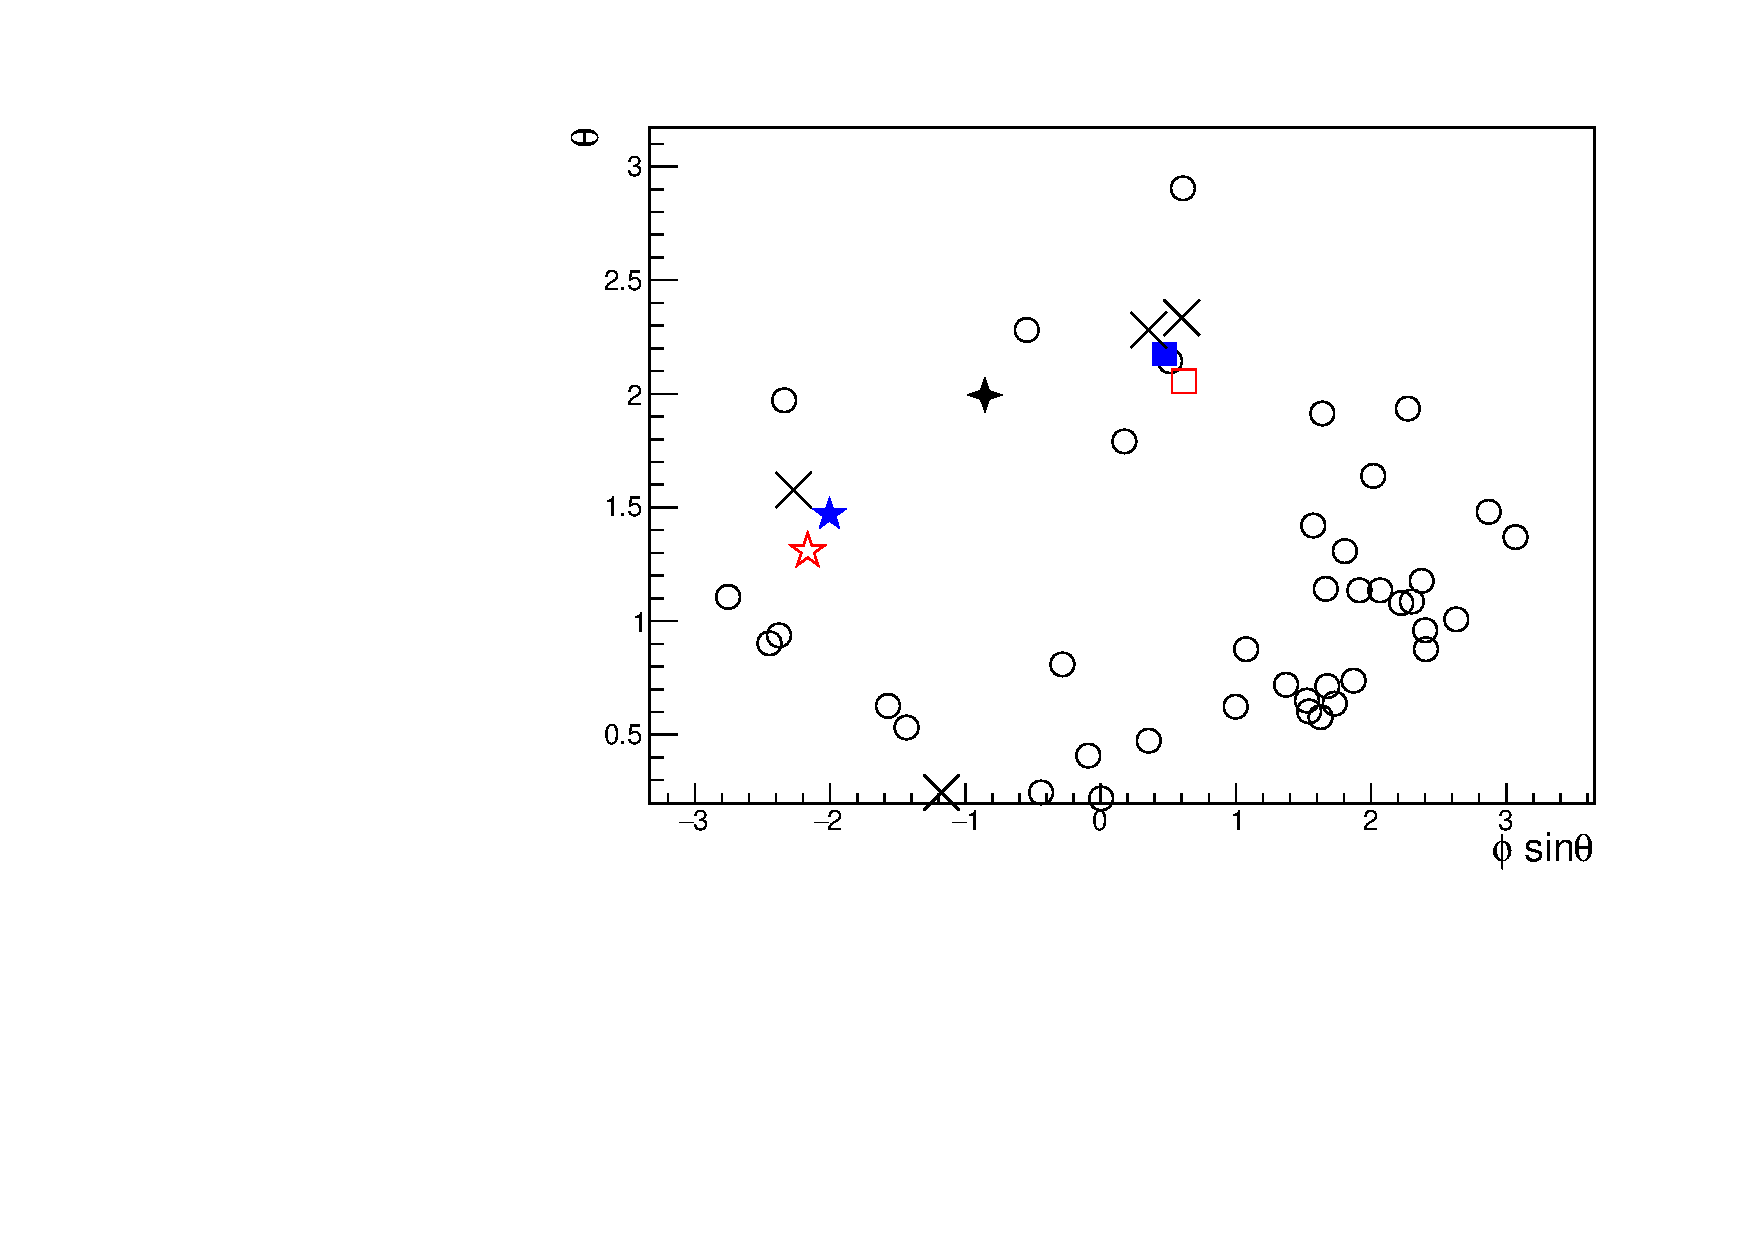
\includegraphics[width=6cm]{PMTmap_100093.pdf}
		\end{minipage}
	}
	\subfigure[Run 100207, GTID 5079885]{ 
		\begin{minipage}[b]{0.4\textwidth}
			\centering
			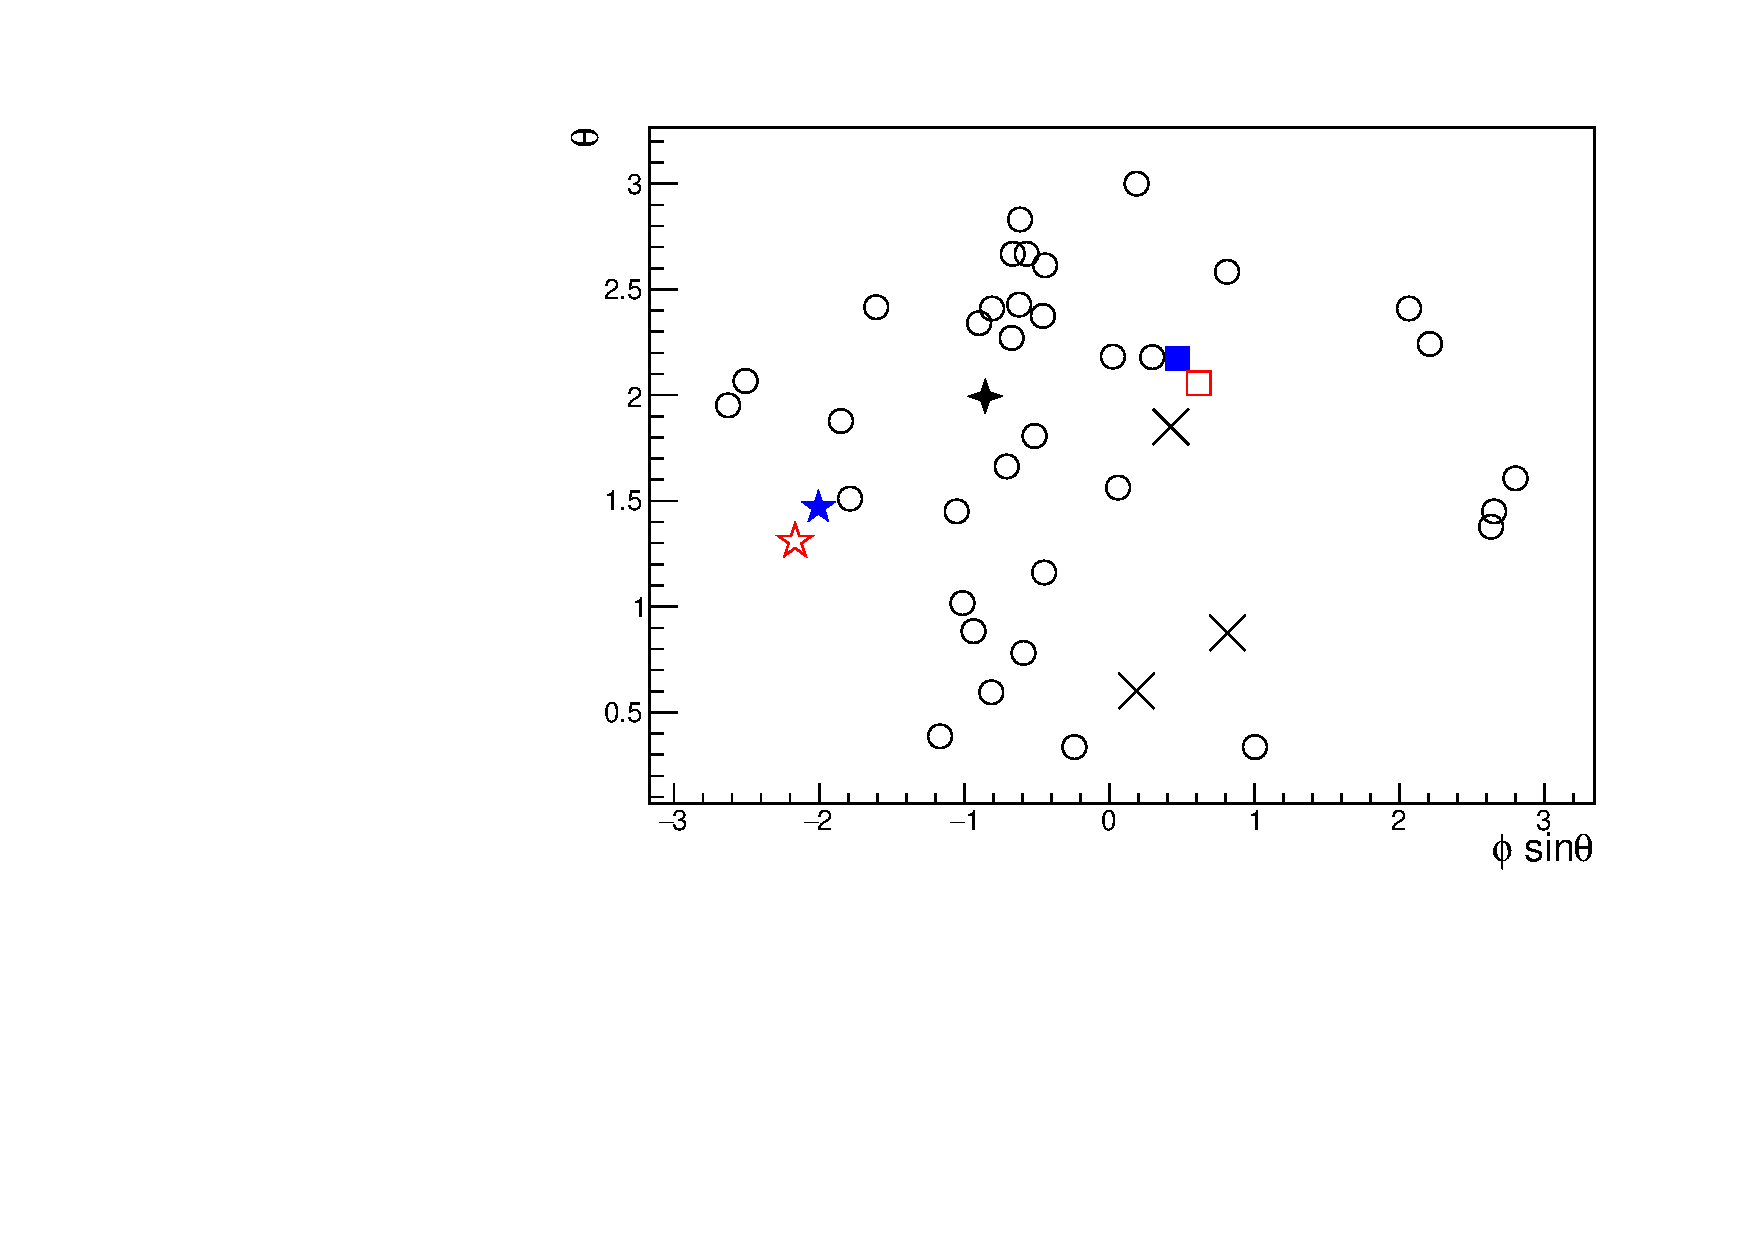
\includegraphics[width=6cm]{PMTmap_100207.pdf}
		\end{minipage}
	}
	\subfigure[Run 100632, GTID 7882360]{ 
		\begin{minipage}[t]{0.4\textwidth}
			\centering
			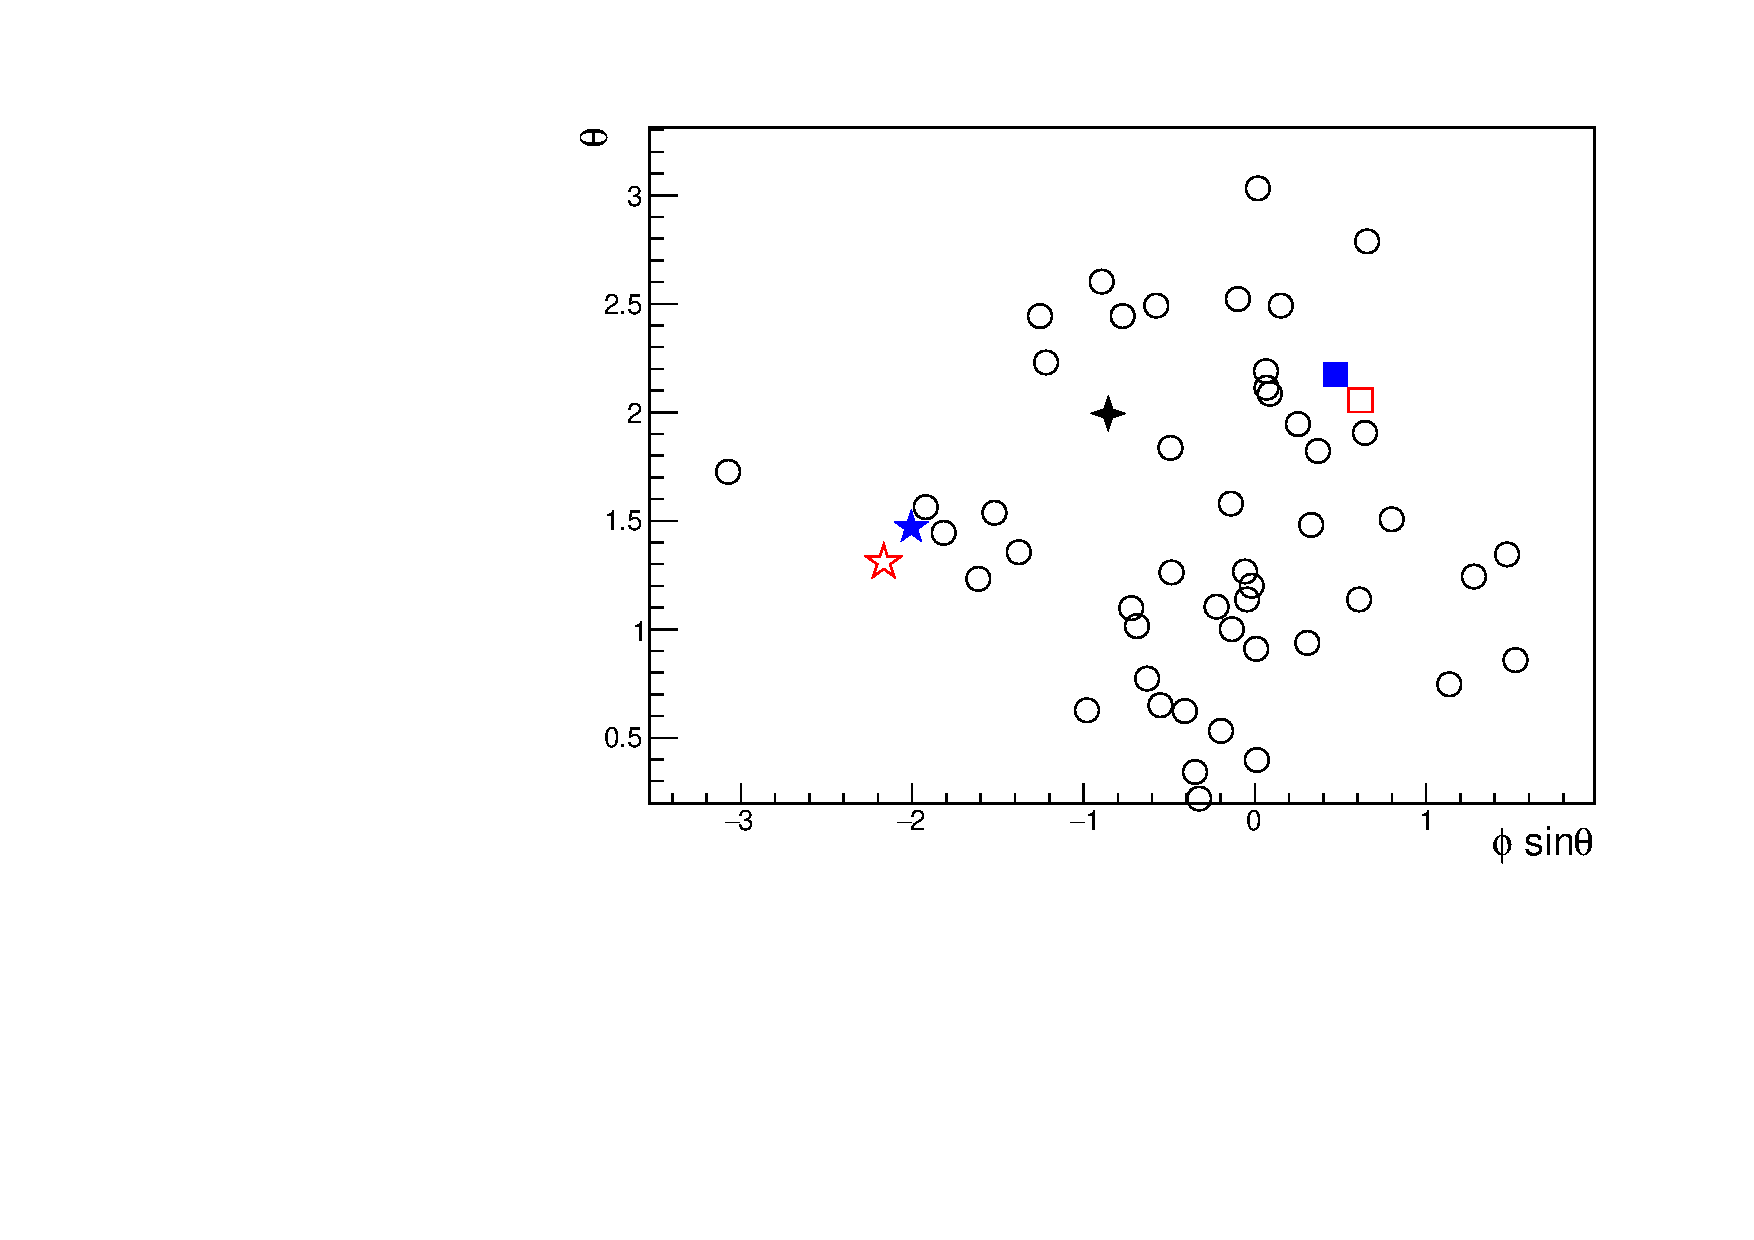
\includegraphics[width=6cm]{PMTmap_100632.pdf}
		\end{minipage}
	}
	\subfigure[Run 100663, GTID 15767175]{ 
		\begin{minipage}[t]{0.4\textwidth}
			\centering
			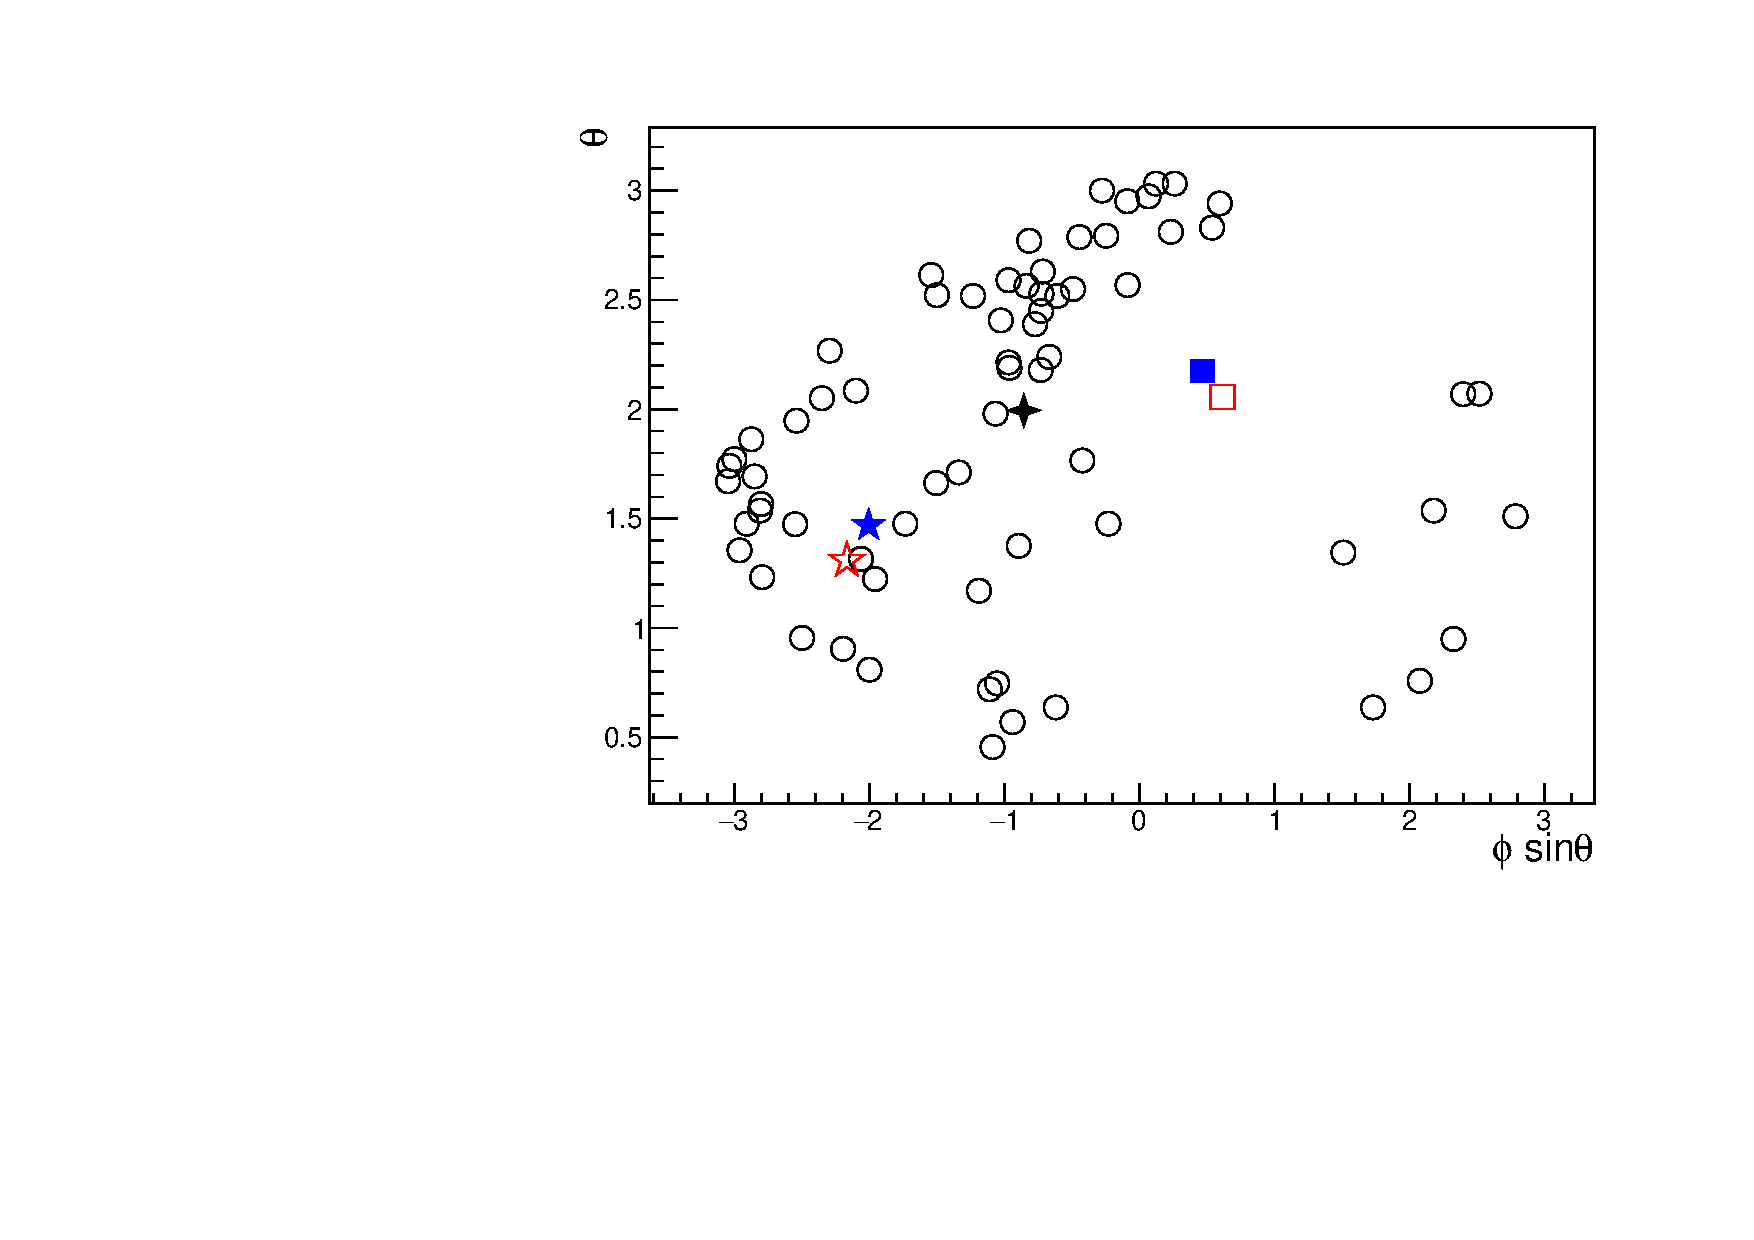
\includegraphics[width=6cm]{PMTmap_100663.pdf}
		\end{minipage}
	}
	\subfigure[Run 100915, GTID 169700]{ 
		\begin{minipage}[t]{0.4\textwidth}
			\centering
			{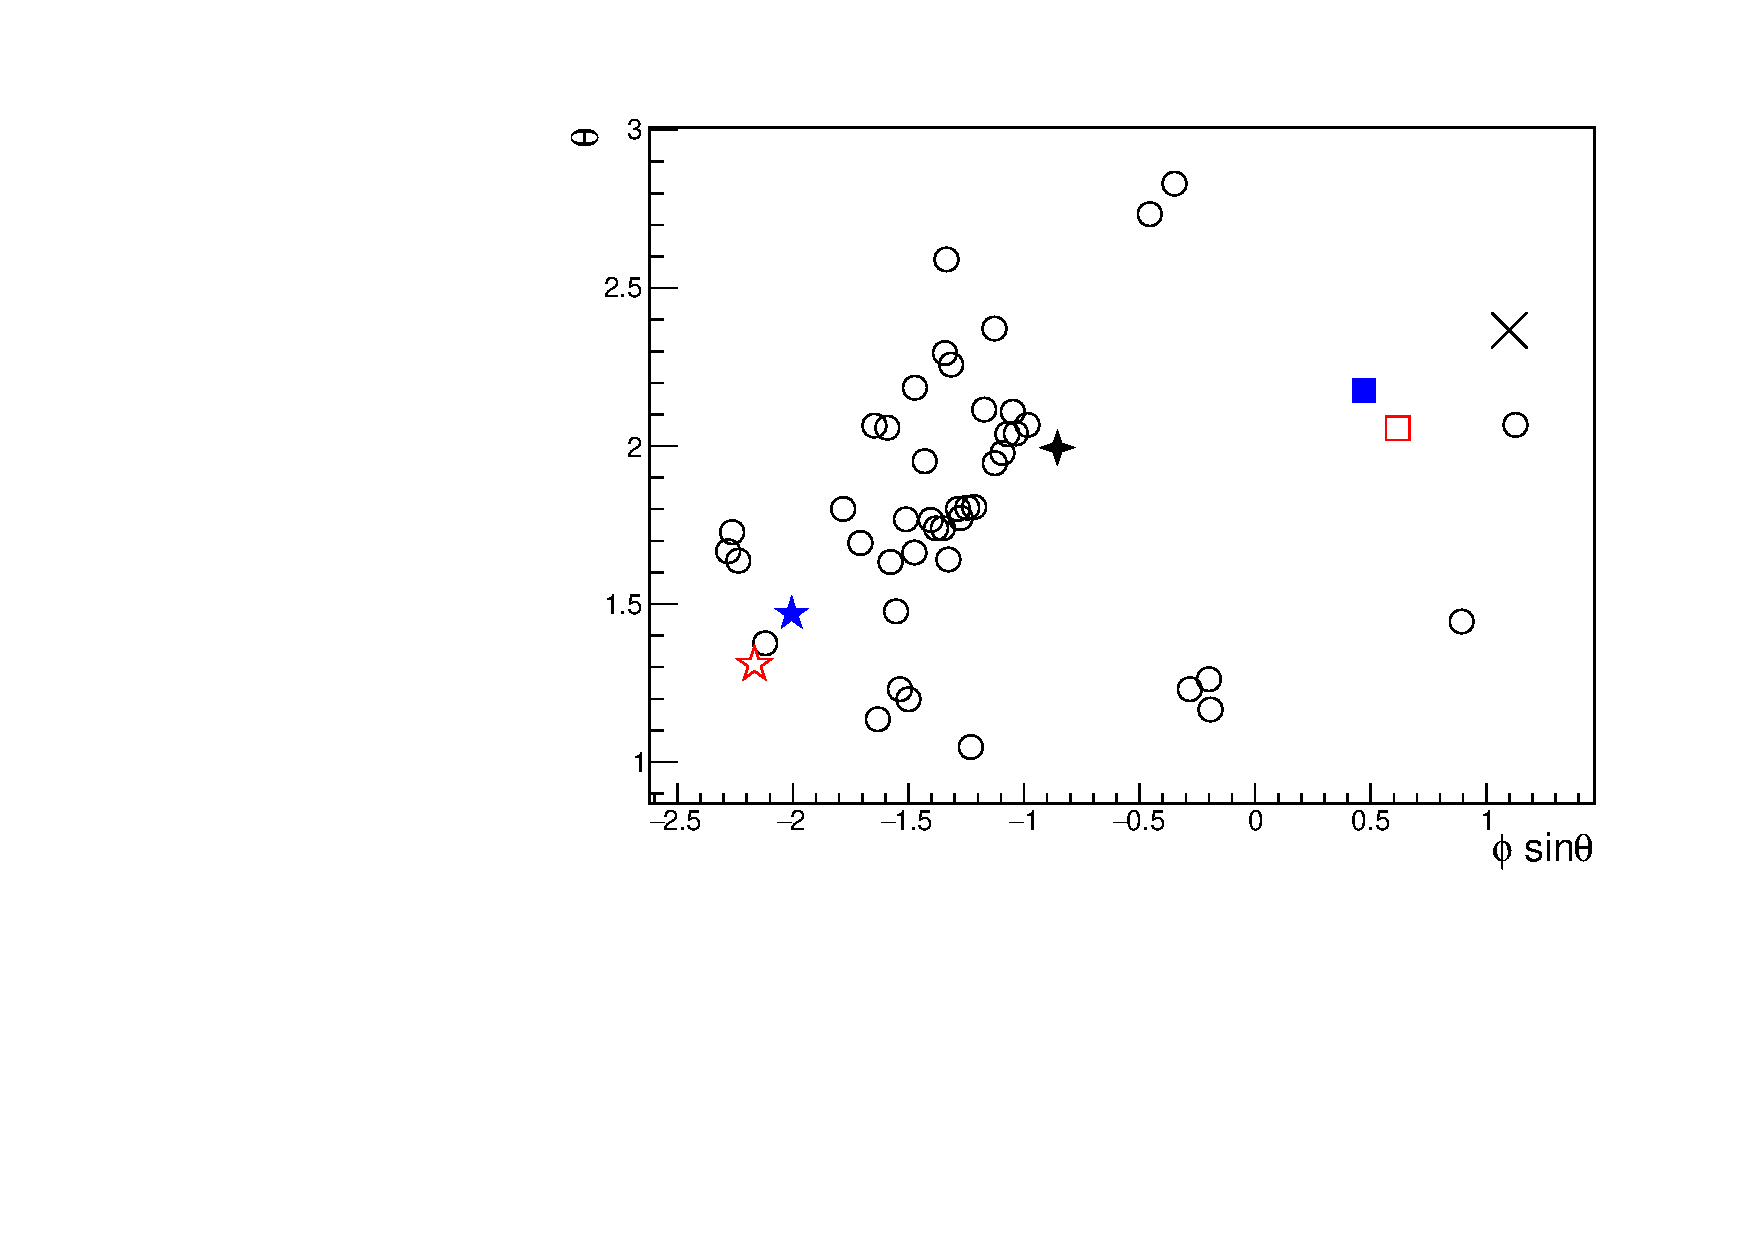
\includegraphics[width=6cm]{PMTmap_100915.pdf}}
		\end{minipage}
	}
	\subfigure[Legends]{ 
		\begin{minipage}[b]{0.4\textwidth}
			\centering
			{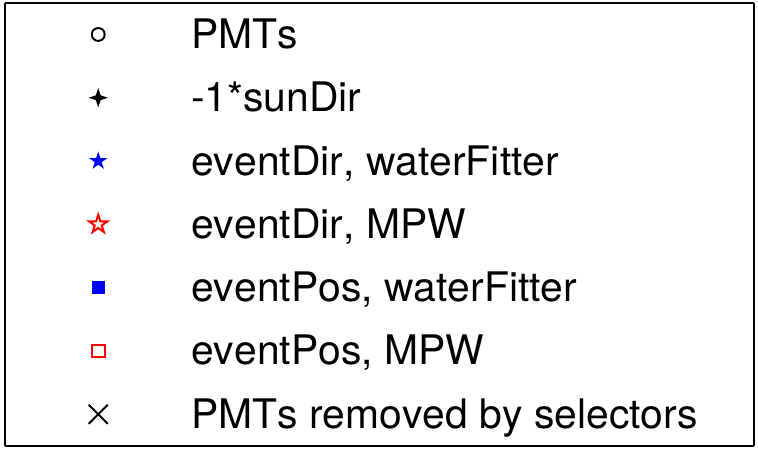
\includegraphics[width=5cm]{solarLegends.png}}
		\end{minipage}
	}
	\caption[Reconstruction results for the candidate events, projected onto PMT sinusoidal maps.]{Reconstruction results for the candidate events, projected onto PMT sinusoidal maps. Black circles stand for the hit PMTs used by the fitter; crosses stand for the hit PMTs removed by the selectors; blue full star stands for the event direction fitted by the \texttt{Rat water fitter}; red open star stands for the direction fitted by the \texttt{MPW fitter}; full double diamond stands for the solar direction*-1; blue full square stands for the event position fitted by the \texttt{Rat water fitter}; open square stands for the position fitted by the \texttt{MPW fitter}.	\label{fig:openDataSetCandidate}}
\end{figure}

From the proximity of the colored points (Fig.~\ref{fig:openDataSetCandidate}) it can be seen that that, for the candidate events, the results from the \texttt{MPW} are largely consistent with those from \texttt{RAT}, although (not apparent from the figure) the \texttt{MPW} fitter disfavored one event in run 100207 (with GTID=5079885), placing its position outside the AV, and the $\cos\theta_\mathrm{sun}$ becomes smaller and is further away from +1. %This event can be checked by looking at the $klDiv$ values (using Eqn.~\ref{eq:symKlDiv}). It gives $klDiv(\mathrm{MPW})=4.95$ and $klDiv(\mathrm{RAT})=9.62$, which indicates that the \texttt{MPW} reconstructed $\cos\theta_\mathrm{Ch}$ distribution is more closer to the nominal Cherenkov angle distribution.

In addition to refitting the candidate events found by the \texttt{RAT}, the \texttt{MPW} fitter can be (and was) used directly to search for candidate events, with the result shown in Table.~\ref{tab:opendataMPW}. Evidently the \texttt{MPW} fitter obtained a different set of candidate events, albeit overlapping with the set provided by the \texttt{RAT} fitter, and so it provides an alternative analysis of the solar neutrinos.
% Compare the $klDiv$ quantities for the \texttt{MPW fitter} and \texttt{Rat water fitter} results. 

\section{Likelihood Fits for Solar Neutrino Candidate Events}

For this section, I focus on the 190.33 live-day low background dataset taken in the second stage of the water phase, with nitrogen cover gas at the top of the neck isolating the newly-filled LAB from lab air. A maximum likelihood fit method for counting the number of the candidate solar neutrino events ($N_{sig}$) and background events ($N_{bkg}$) in a dataset is discussed. To check the method, the dataset from the run-200004 to 203602 was used. This dataset has a live time of 92.54 days, about a half of the whole 190.33 live-day dataset, so it is denoted as the ``half-dataset''. The actual data and the run-by-run MC simulations of this half-dataset were used for testing the analyses in this section and the next.

Before the analysis, the following ``beforehand cuts'' were applied: 
\begin{itemize}
    \item NHits$>20$, 
    \item $R'_{fit}<5500 \; \mathrm{mm}$,
    \item ITR$>0.55$,
    \item $-0.12<\beta_{14}<0.95$. 
\end{itemize}
Here NHits$>20$ is a reconstruction threshold set for the solar neutrino analysis, which means that only the events with NHits$>20$ were reconstructed by the \texttt{MPW fitter}. The $R'_{fit}$ is the magnitude of the reconstructed event position $\vec{X}_{fit}$ after the AV coordinate correction:
\begin{equation*}
R'_{fit}\equiv\sqrt{x^2_{fit}+y^2_{fit}+(z_{fit}-108)^2}
\end{equation*}
(the 108 mm offset in $z$ was discussed in Chapter 3 and Chapter 4.). The cut on $R'_{fit}$ defines a fiducial volume of $5500$ mm for solar neutrino analysis. Finally, the high level cuts ITR and $\beta_{14}$ cuts were mentioned previously.

\subsection{Maximum Likelihood Fit}\label{sect:poisson_fit}

To prepare for the fit, the values of the solar angle, $\cos\theta_\mathrm{sun}$ from the data were filled into a histogram covering a range of [-1,1] with 40 bins. For each bin, the observed event count ($n_{obs}$) was considered as a sum of solar $\nu_e$ and background events. The count in each bin was assumed to follow a Poisson distribution: $Poisson(n_{obs}, N_{bkg} \, P_{bkg}+N_{sig} \, P_{ES}(E))$, where $P_{bkg}$ and $P_{ES}(E)$ are the assumed distributions of background events and solar $\nu_e$ events respectively.

For background events, a uniform distribution of $\cos\theta_\mathrm{sun}$ was assumed. On the other hand, $\cos\theta_\mathrm{sun}$ distributions for solar $\nu_e$ events were extracted from the realistic run simulations after applying the beforehand cuts, as shown in Fig.~\ref{solarPDF}. 

\begin{figure}[!htb]
	\centering
	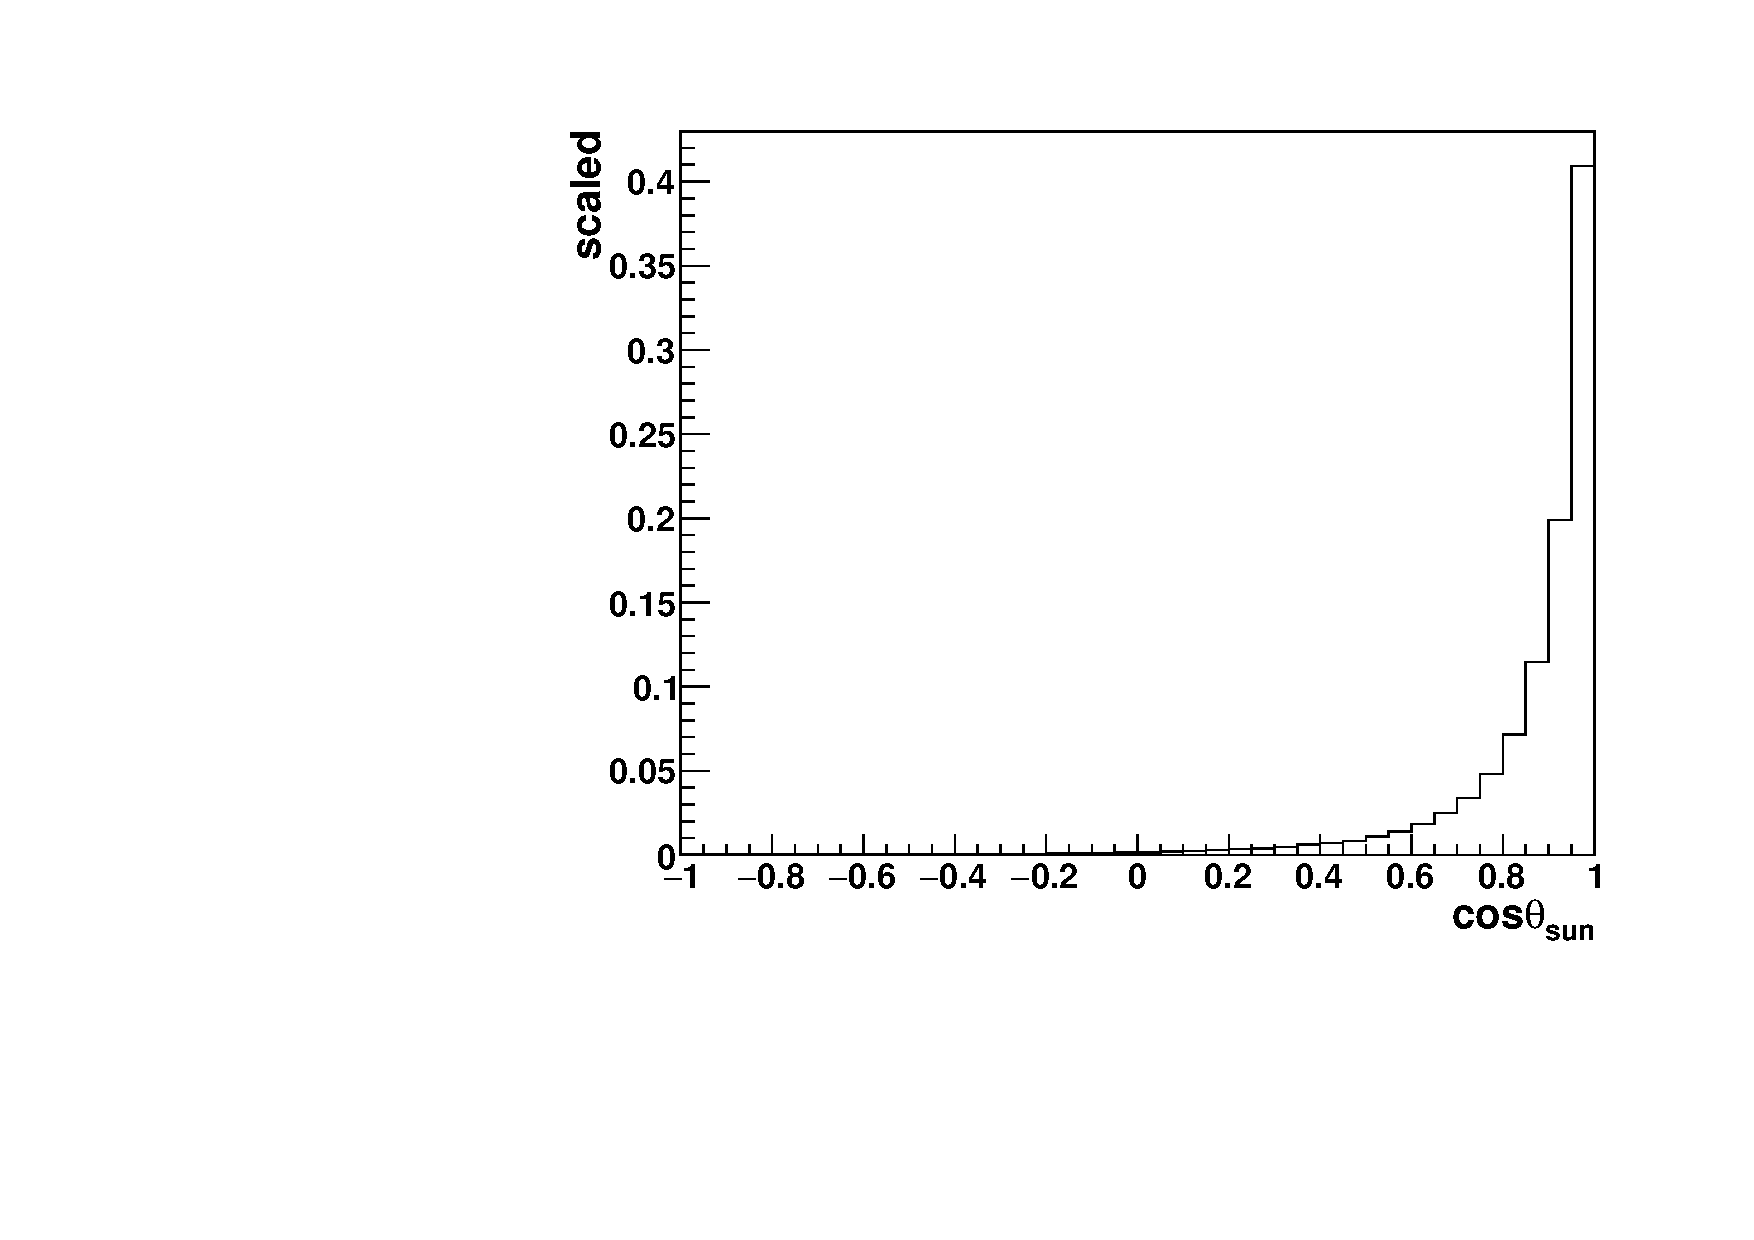
\includegraphics[width=8cm]{solarPDF.pdf}
	\caption[The $\cos\theta_\mathrm{sun}$ distribution of solar $\nu_e$ used as a PDF function.]{The $\cos\theta_\mathrm{sun}$ distribution for solar $\nu_e$ events extracted from the simulations, which is scaled (so as to have an integral of 1) to obtain a probability density function.}
	\label{solarPDF}
\end{figure}

Adding up each bin $i$ and taking $N_{bkg}$ and $N_{sig}$ as the free parameters for fitting, the maximum likelihood function was built as \cite{pdg2020}:

\begin{equation}\label{eq:solar_poissonFitMinimizer}
-2\ln\mathcal \lambda(N_{sig},N_{bkg})
=2\sum_{i=0}^{N_{bins}}[\mu_i(N_{sig},N_{bkg})-n_i+n_i\ln\frac{n_i}{\mu_i(N_{sig},N_{bkg})}],
\end{equation}
where $\mu_i(N_{sig},N_{bkg})$ is the expected number of events in each bin
\begin{equation*}
\mu_i(N_{sig},N_{bkg})=N_{sig}\cdot P^i_{ES}(E^i)+N_{bkg}\cdot\frac{1}{N_{bins}}\,
\end{equation*}
and $N_{bins}$ is the total number of the bins, usually taken as 40 (for a bin width of 0.05 covering -1 to 1). The calculation of Eqn.~\ref{eq:solar_poissonFitMinimizer} includes the cases when the bin contains zero ($n_i=0$).

Fitting the data with $(N_{bkg},N_{sig})$ by maximizing the quantity $-2\ln\mathcal\lambda$, the best fit for $N_{bkg}$ and $N_{sig}$ was obtained. In the next section, an ensemble test based on fake datasets was applied to test the fit performances.
%Fig.~\ref{solarFits1} shows the fit results. The fitted number of solar $\nu_e$ events is $N_{sig} = 67.1\pm9.2$, which is equivalent to a rate of $1.04\pm 0.14~event/(day\cdot kiloton)$; while the fitted number of background events is $N_{sig} = 3.4\pm0.91$, which is equivalent to a rate of $0.05\pm 0.01 event/(day\cdot kiloton)$.
%
%\begin{figure}[!htb]
%	\centering
%	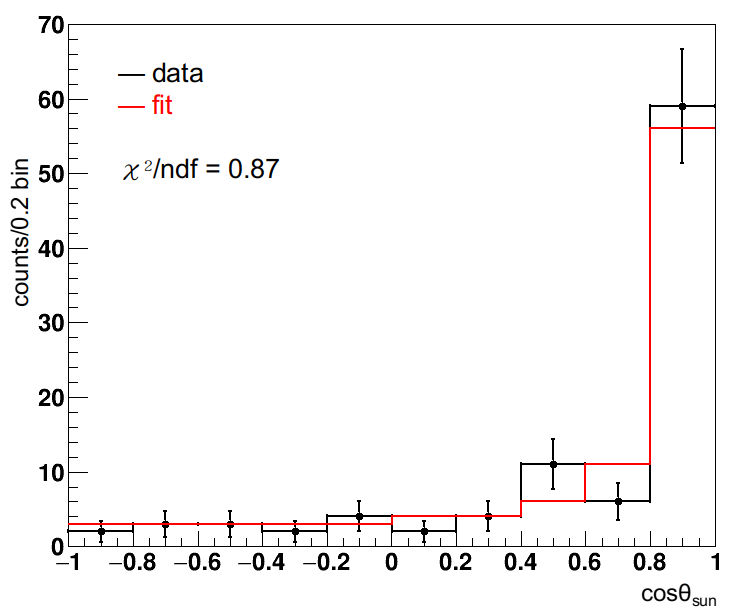
\includegraphics[width=8cm]{solarFits1.png}
%	\caption{Fit results for the $N_{bkg}$ and $N_{sig}$ via the maximum likelihood method.}
%	\label{solarFits1}
%\end{figure}
%
%2D fits
\subsection{Ensemble Test}\label{sect:ensemble}

To check the uncertainty of the Poisson fit, a method similar to that of Ref.~\cite{leta} was used. 5000 fake datasets were generated from the run-by-run MC simulations of the 92.54 live-day half-dataset (runs 200004 to 203602). The `beforehand cuts' had been applied to these simulations.
%In the MC dataset, for $E_{fit}>5$~MeV, there were 6359 backgrounds from different background events and 317205 signals of internal solar $\nu_e$ events (the event types were mentioned in Table.~\ref{table:mixed_MC}).

The number of background events in a fake dataset, $N^f_{bkg}$, was assumed to be twice the event number in the $-1<\cos\theta_\mathrm{sun}<0$ region, while the number of signal events $N^f_{sig}=N^f_{total}-N^f_{bkg}$. These numbers were determined from the actual data, rather than the simulations. Fig.~\ref{half_data} shows the actual data of the half-dataset, after the data-cleaning cuts and beforehand cuts. Reading from the actual data, it found $N^f_{bkg}=38$ and then $N^f_{sig}=109-N^f_{bkg}=71$. To do the ensemble test, for each fake dataset, two random numbers: $N^r_{sig}$ and $N^r_{bkg}$ were generated by the $\texttt{ROOT TRandom3}$ random number generator class. Each of the two random numbers followed the random Poisson distribution: $e^{-\mu}\mu^{N^r}/N^r!$, where $\mu=71$ or $38$, and thus they fluctuated around $N^f_{sig}$ or $N^f_{bkg}$.

\begin{figure}[!htb]
	\centering
	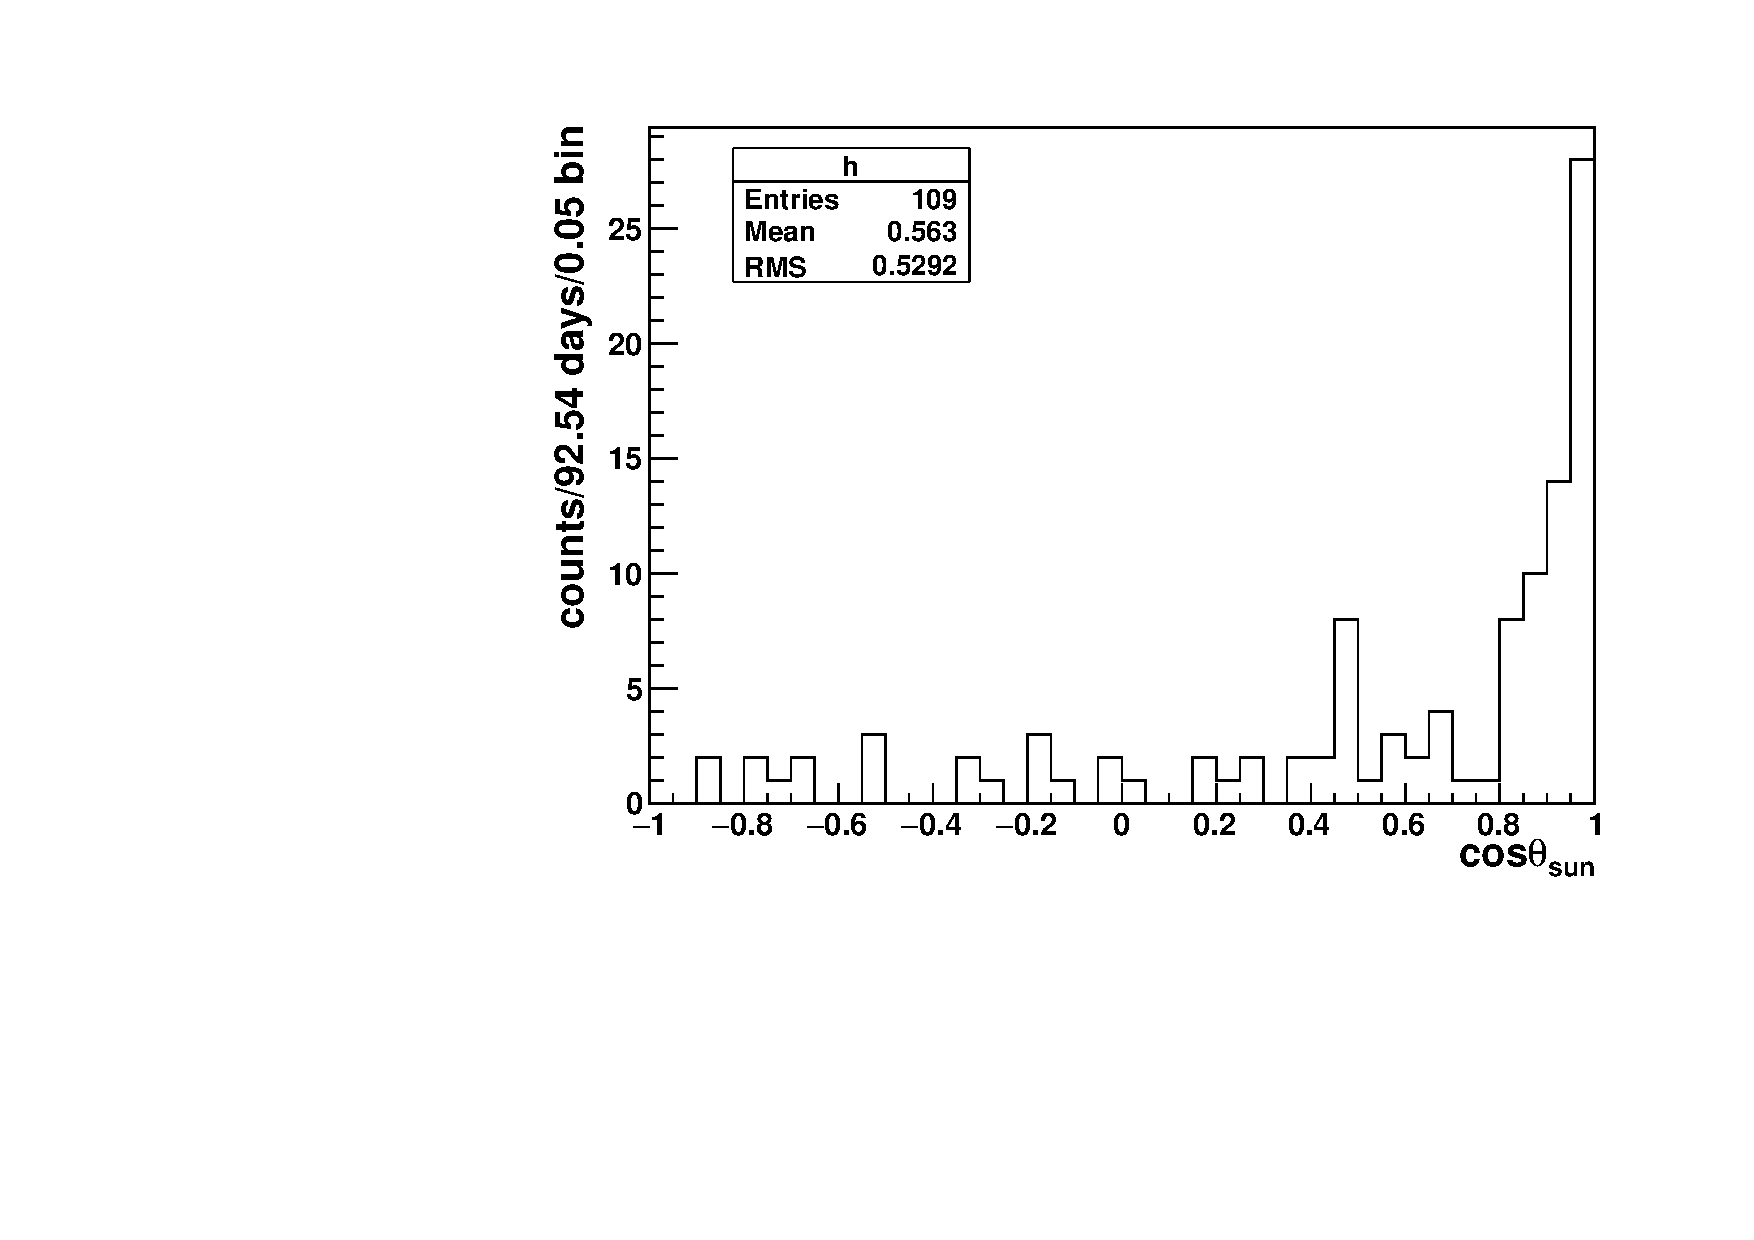
\includegraphics[width=10cm]{cosThetaToSun_halfData_5to15.pdf}
	\caption[Real data from run-200004 to 203602 (half-dataset), after the beforehand cuts.]{Real data from run-200004 to 203602 (half-dataset), after the beforehand cuts. The number of counts in the $-1<\cos\theta_\mathrm{sun}<0$ region is 19.}
	\label{half_data}
\end{figure}

To create the fake datasets, from the solar $\nu_e$ MC simulations, $N^r_{sig}$ events which passed the cuts were randomly selected; similarly, from the merged background simulations, $N^r_{bkg}$ events were randomly selected. These randomly selected events were merged into a fake dataset, and their values of $E_{fit}$ and $\cos\theta_\mathrm{sun}$ were recorded.
By repeating the random selection, an ensemble of fake datasets were created. Each fake dataset was fitted with the maximum likelihood function described in Sect.~\ref{sect:poisson_fit}. Fig.~\ref{ensemble_test} shows an example of the fit results from a random fake dataset.

\begin{figure}[!htb]
	\centering
	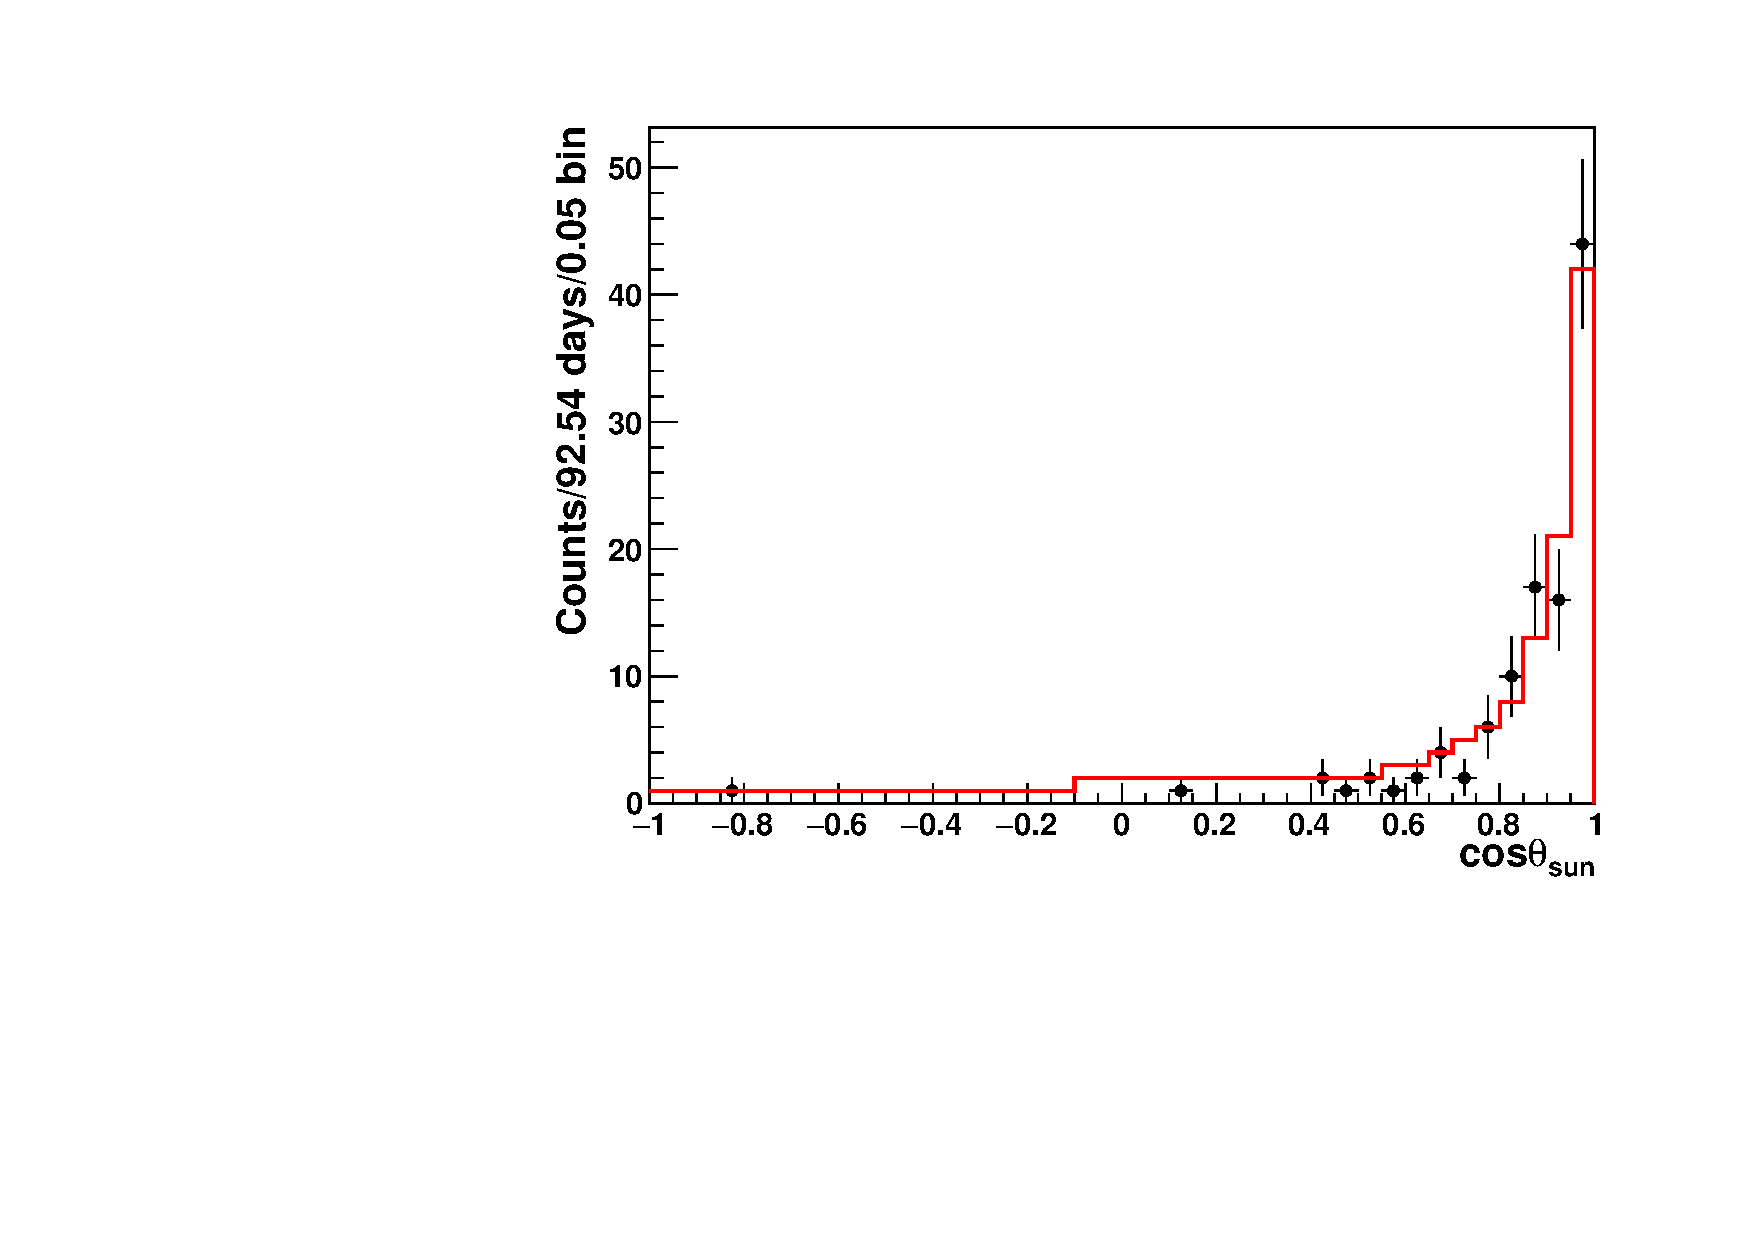
\includegraphics[width=10cm]{ensemble_fitExample.pdf}
	\caption[An example of the $\cos\theta_\mathrm{sun}$ distribution from a fake dataset fitted with $(N_{sig},N_{bkg})$.]{An example of the $\cos\theta_\mathrm{sun}$ distribution from a fake dataset fitted with $(N_{sig},N_{bkg})$. The black dots are data points and the red line shows the fit. For $N^r_{sig} = 73$ and $N^r_{bkg}=44$, the fit results are $N_{sig} = 73.42\pm9.42$ and $N_{bkg} = 43.58 \pm 7.73$, with a $\chi^2/ndf = 60.19/40 = 1.50$.}
	\label{ensemble_test}
\end{figure} 

The fit pull and the fit bias were defined by \cite{leta}:
\begin{equation}
\mathrm{bias}=\frac{N_{sig}-N^r_{sig}}{N_{sig}},
\end{equation}

\begin{equation}
\mathrm{pull}=\frac{N_{sig}-N^r_{sig}}{\sigma_{sig}},
\end{equation}
where $N_{sig}$ is the fitted number of signal events, $\sigma_{sig}$ is the statistical uncertainty of $N_{sig}$; $N^{r}_{sig}$ is used as the true number of signal events in the fake dataset.

Fig.~\ref{poisson_fitPull} and Fig.~\ref{poisson_fitBias} show the fit pull and bias respectively. The histograms were fitted with Gaussians. For the fitted number of signal events, the Gaussian mean of the fit biases is $-0.0044\pm0.0008$ for 5000 fake datasets while the Gaussian mean of the fit pulls is $-0.026\pm0.006$. These pulls and biases will be applied on the data. Fig.~\ref{poisson_fitLnL} shows the distribution of $-2\ln L$ (the log likelihood is calculated according to Eqn.~\ref{eq:solar_poissonFitMinimizer}) returned by the best fit result ($-2\ln L_{best}$) for each fake dataset. The distribution, $f({-2\ln L_{best}})$, follows the asymptotic $\chi^2$ PDF with a degree of 40 and is used to compute the $p-\mathrm{value}$s \cite{pdg2020}. For a best-fit set ($N^i_{sig},N^i_{bkg}$) with a value of $-2\ln L^i_{best}$, the $p-\mathrm{value}$ is calculated as
\begin{equation*}
p=\int_{-2\ln L^{i}_{best}}^{-2\ln L^{max}_{best}}f({-2\ln L_{best}}) \; d(-2\ln L_{best}) \; .
\end{equation*}


\begin{figure}[!htb]
	\centering
	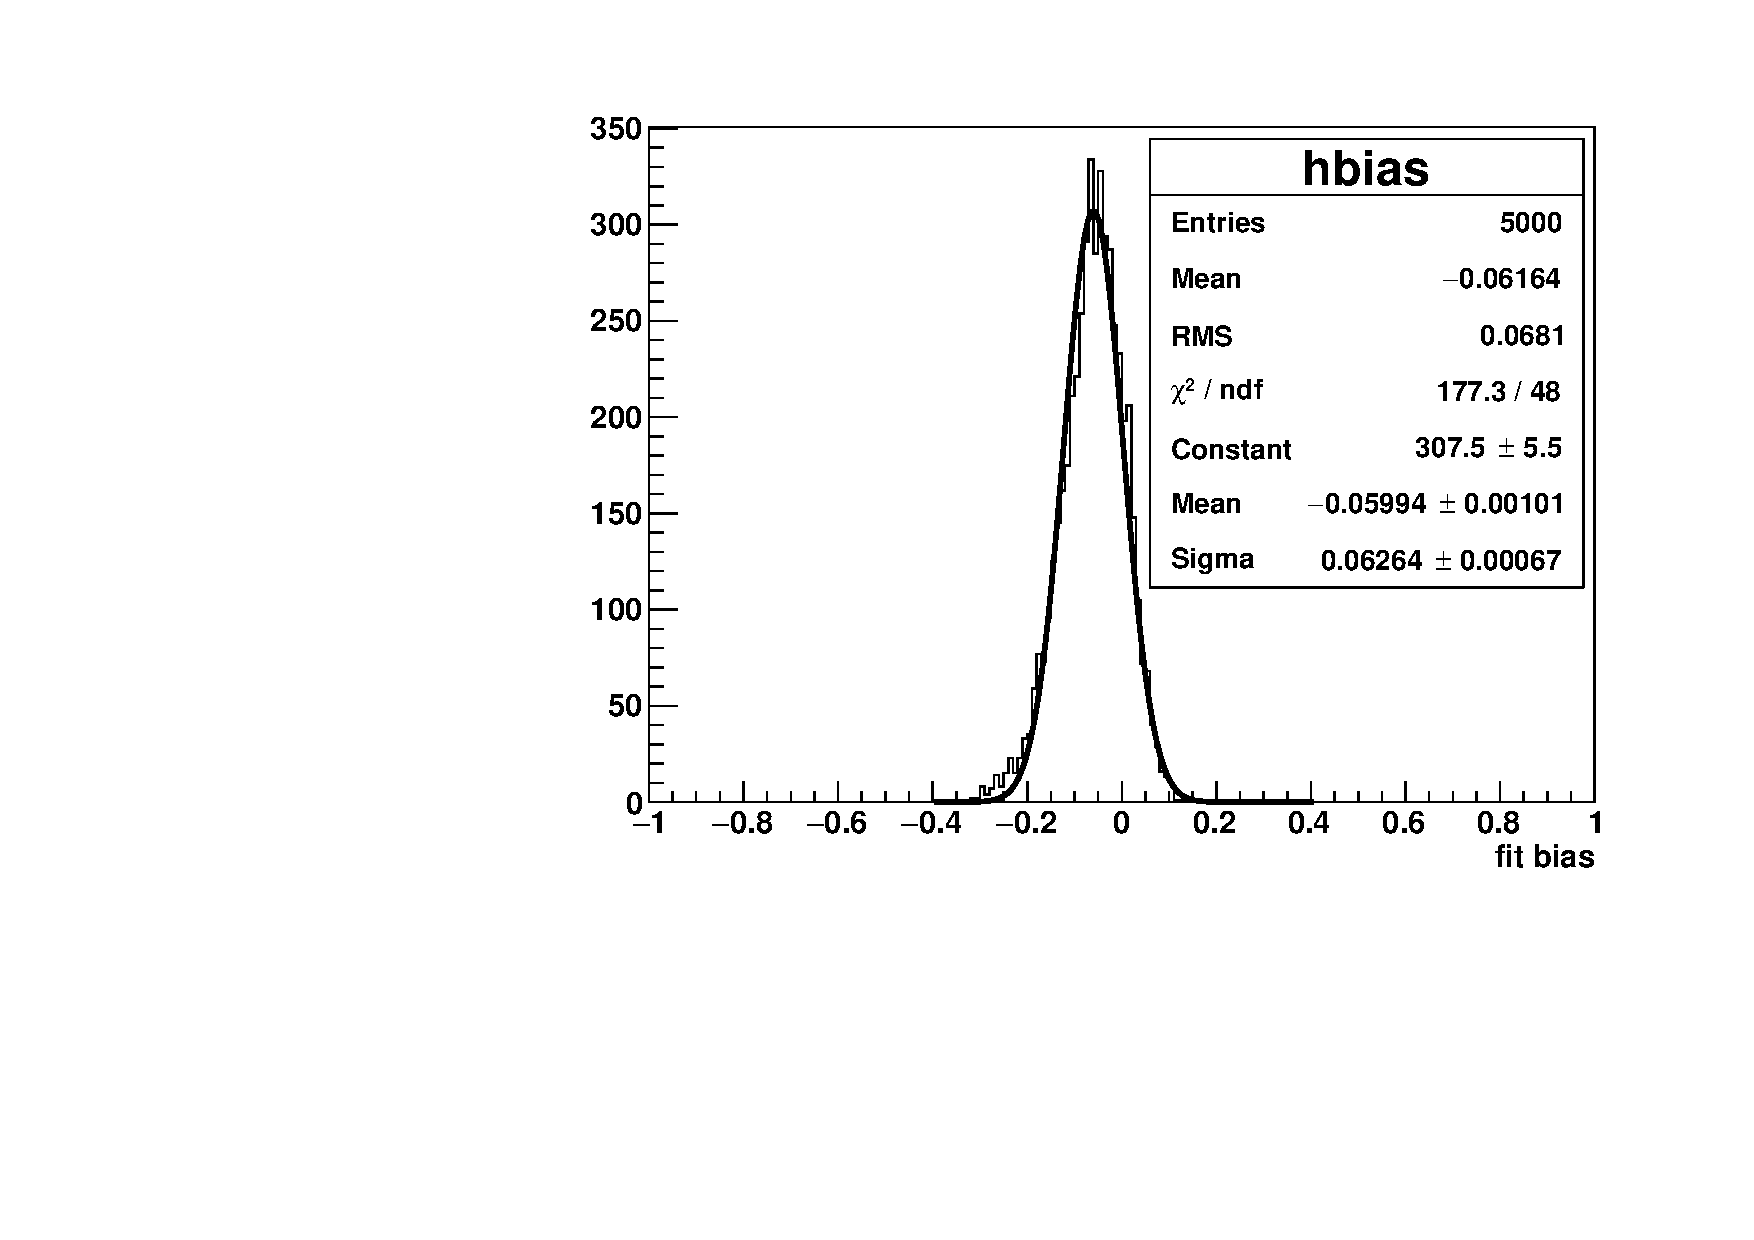
\includegraphics[width=8cm]{ensemble_fitBias.pdf}
	\caption{$N_{sig}$ fit biases for 5000 fake datasets.}
	\label{poisson_fitBias}
\end{figure} 

\begin{figure}[!htb]
	\centering
	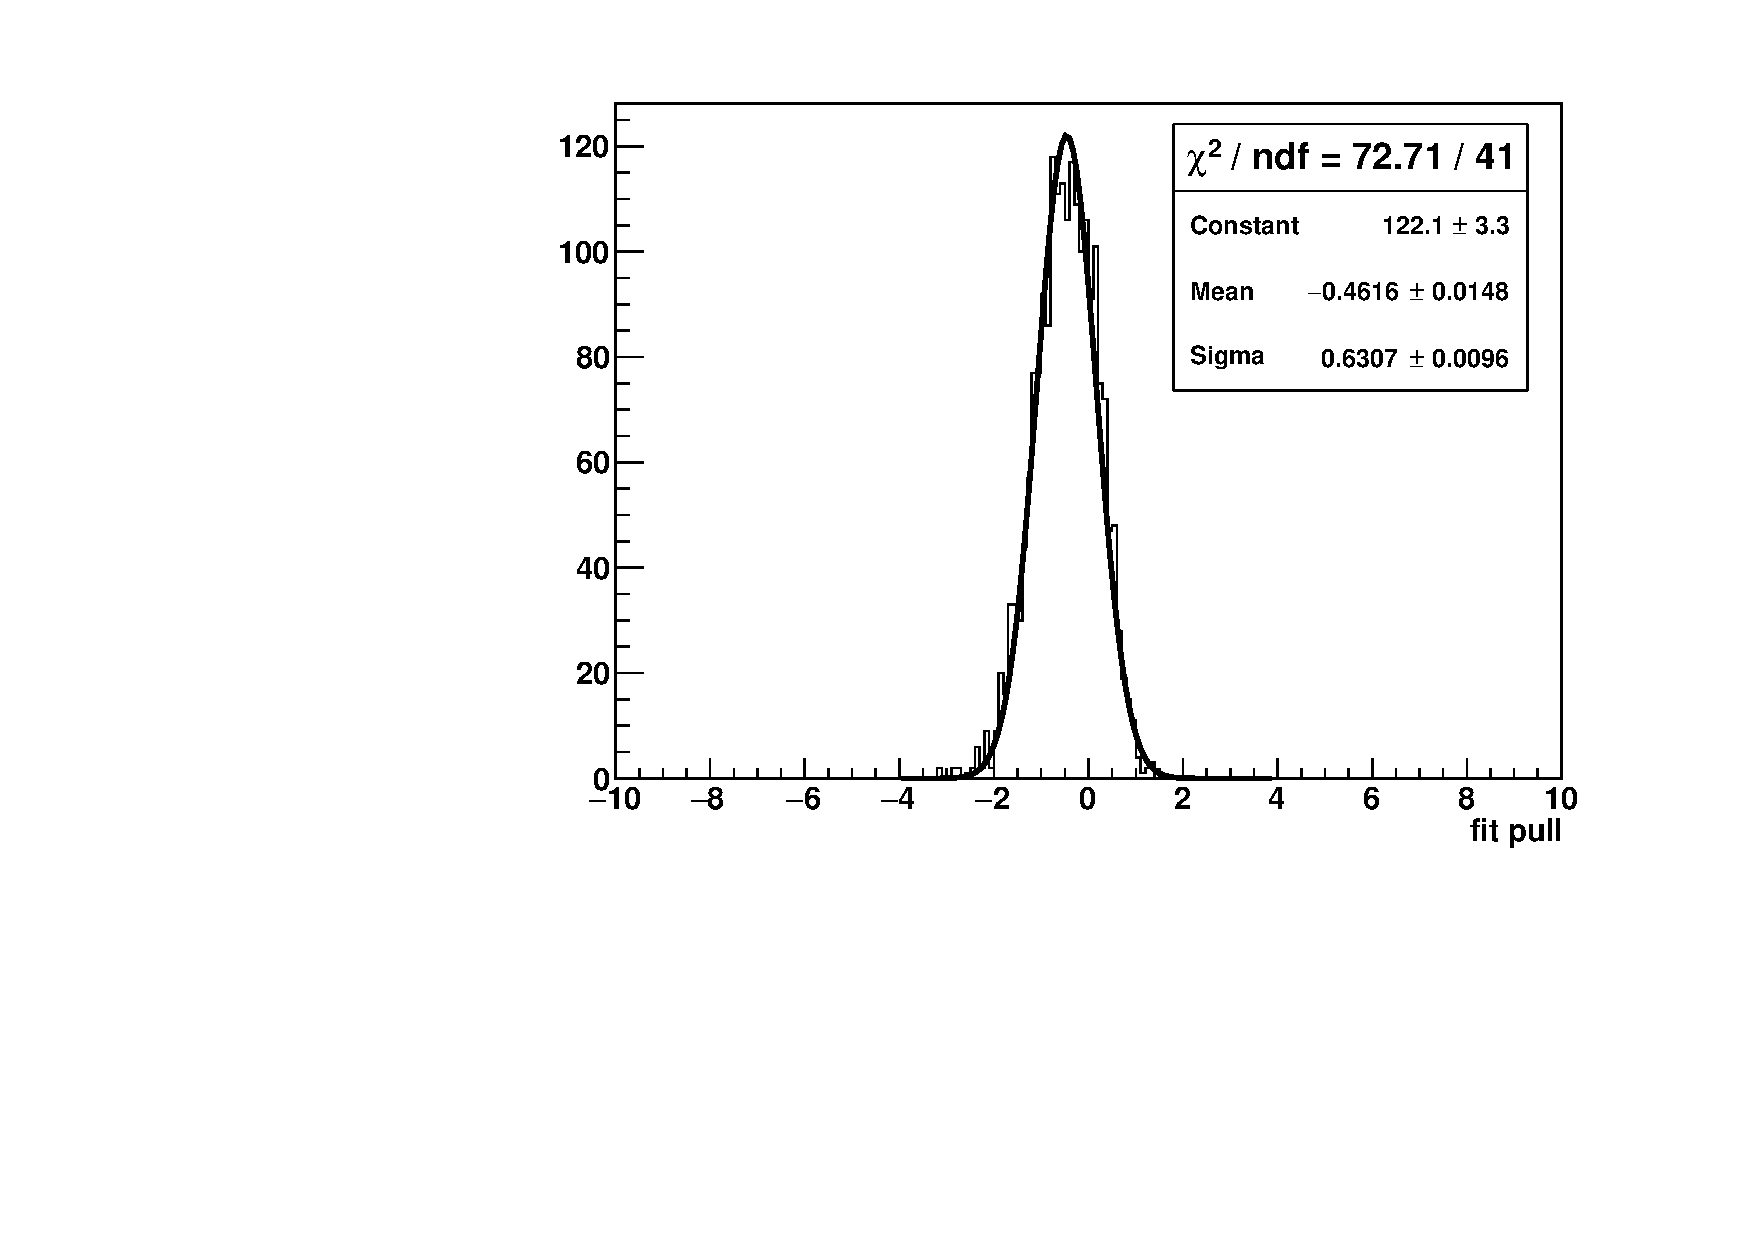
\includegraphics[width=8cm]{ensemble_fitPull.pdf}
	\caption{$N_{sig}$ fit pulls for 5000 fake datasets.}
	\label{poisson_fitPull}
\end{figure} 

\begin{figure}[!htb]
	\centering
	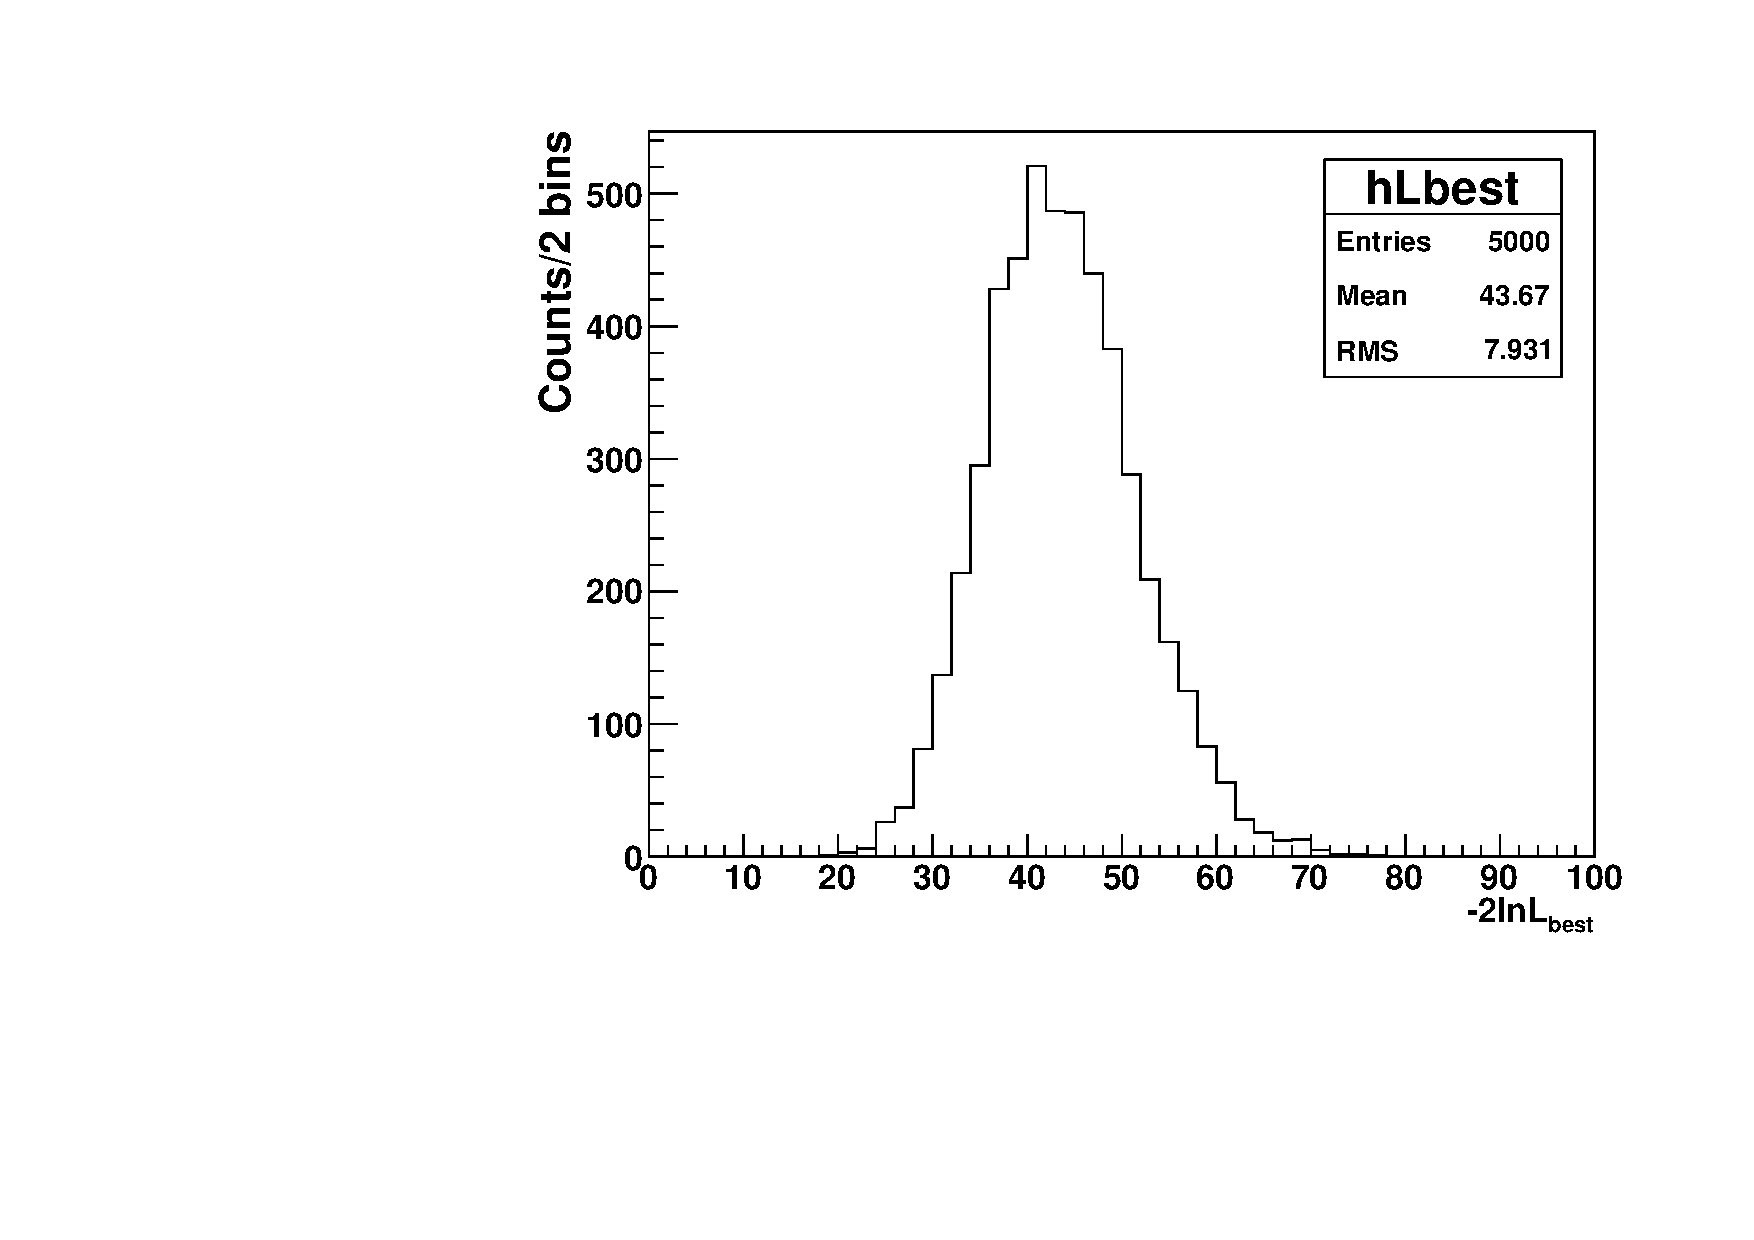
\includegraphics[width=8cm]{ensemble_lnLbest.pdf}
	\caption{The $-2\ln L$ distribution of the best fit results from the 5000 fake datasets.}
	\label{poisson_fitLnL}
\end{figure}

\subsection{Kullback–Leibler Divergence for High Level Cuts}

For the solar neutrino analysis, I used a quantity called ``Kullback–Leibler (KL) divergence'' (also called ``relative entropy'') as a new quantity to calculate the dissimilarity between a reconstructed event and a simulated solar neutrino event, and then to classify the possible solar neutrino event and the background event. Generally, the KL divergence is used to measure the dissimilarity of two probability distributions \cite{murphy2012machine}. The angle $\theta_\mathrm{Ch}$ between the reconstructed event orientation $\vec{u}_{fit}$ and the line joining fitted event position $\vec{X}_{fit}$ to PMT position is given by:
\begin{equation*}
\cos\theta_\mathrm{Ch}=\vec{u}_{fit} \, \cdot \, \frac{\vec{X}_{PMT}-\vec{X}_{fit}}{|\vec{X}_{PMT}-\vec{X}_{fit}|} \; ,
\end{equation*}
and this angle is compared with the averaged angular distribution of solar $\nu_e$ events extracted from the MC simulations (with the reconstructed $\vec{u}$ and $\vec{X}$ from MC), which is set as the nominal distribution. According to the simulations, the solar $\nu_e$ events produce nice Cherenkov angular distribution, which is peaked around the Cherenkov angle ($\theta_\mathrm{Ch}\sim 0.75$). On the other hand, background events with energies below 5 MeV may have smeared angular distributions. The dissimilarity of the event distribution to be investigated and the nominal distribution is calculated. The quantity $klDiv(p||q)$ is calculated as: 
\begin{equation}\label{eq:kldiv}
klDiv(p||q) \equiv \sum_{i}^N p(x_i)\log{\frac{p(x_i)}{q(x_i)}},
\end{equation}
where $p(x_i)$ is the angular distribution after a time residual window cut: $-5<t_{Res}<1~ns$, to extract prompt Cherenkov lights. Both of the event and the MC distributions were filled into a histogram with 40 bins ranging from [-1,1] and the $klDiv$ values were calculated bin by bin excluding the empty bins (zero count). A small $klDiv$ value indicates a small dissimilarity.

These values were used for distinguishing the signal from backgrounds, which will be discussed in the Sect.~\ref{sect:tmva}. Fig.~\ref{kLdiv_example} shows an example of the $klDiv$ calculation. Two events are compared here: one is a randomly selected event from the solar $\nu_e$ run-by-run MC ($E=4.78$~MeV), the other is from the $^{214}$Bi MC ($E=2.18$~MeV), with the same event GTID. Their $\cos\theta_\mathrm{Ch}$ distributions were scaled to the nominal one. It can be seen that the background event with lower energy is more dispersive while the signal event has a peak around the Cherenkov angle, and thus its shape is more close to the PDF. The calculation of \ref{eq:kldiv} gives $klDiv(\mathrm{solar}~\nu_e)=11.78$ and $klDiv(^{214}\mathrm{Bi})=22.69$, which verifies the observation.

\begin{figure}[!htb]
	\centering
	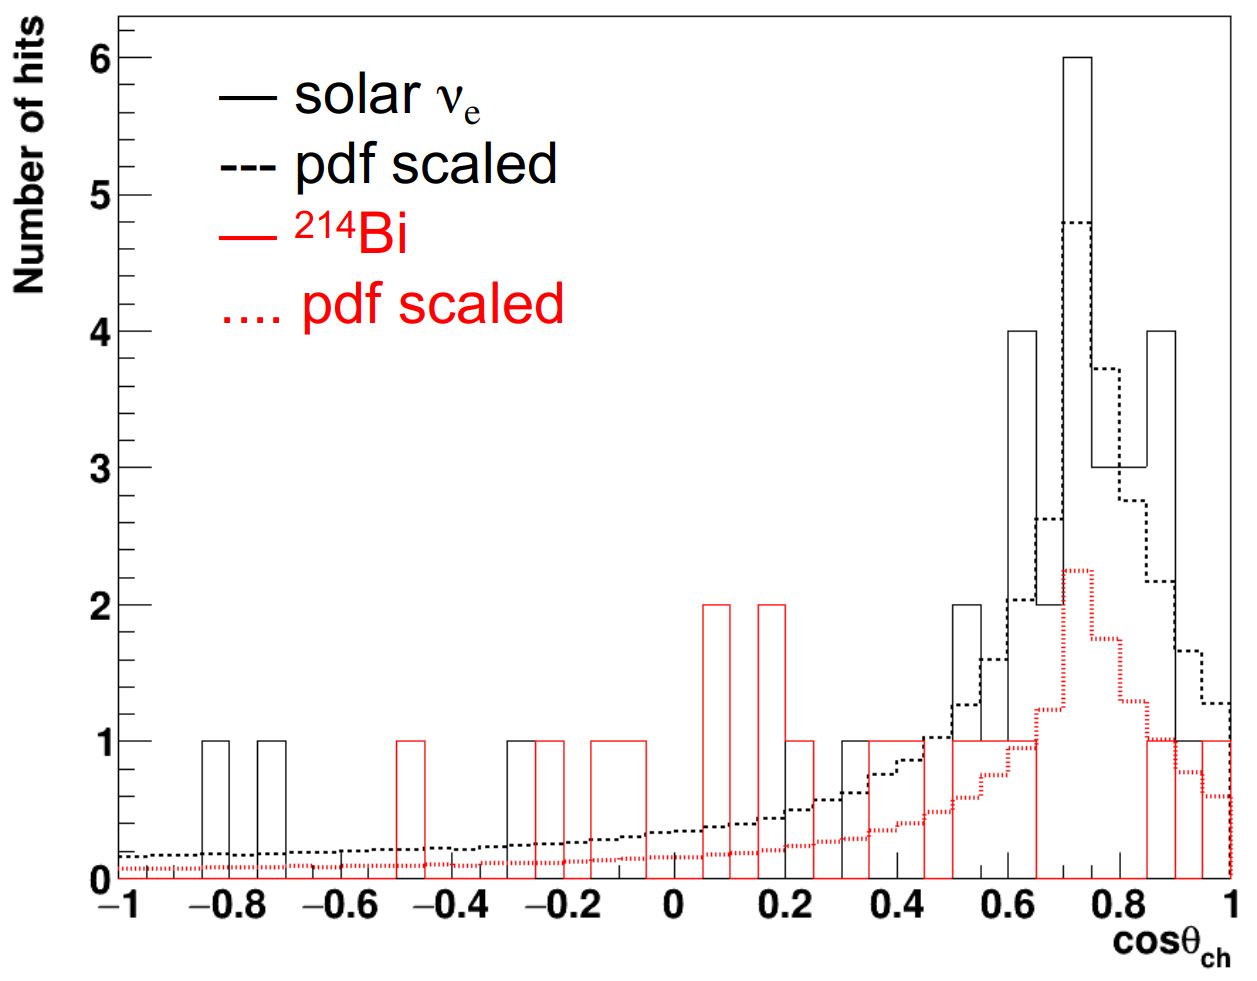
\includegraphics[width=8cm]{klDiv_example.png}
	\caption[Angular distributions of the MC events in run-by-run simulations.]{Angular distributions of the MC events in run-by-run simulations of run-206391, with the same event (GTID = 7). The black line is the MC solar $\nu_e$ distribution, while the red line is the MC $^{214}$Bi distribution. The PDF is scaled to the number of the hits in solar $\nu_e$ event (dashed black line) and the $^{214}$Bi event (dotted red line) respectively.}
	\label{kLdiv_example}
\end{figure}

A symmetrical form of $klDiv$ can be taken as:
\begin{equation}\label{eq:symKlDiv}
klDiv(p,q) \equiv \frac{1}{2}\sum_{i}^N (p\log{\frac{p}{q}}+q\log{\frac{q}{p}}),
\end{equation}
Since $klDiv(p,q)=klDiv(q,p)$, it has a meaning of distance. This symmetric quantity is used in the TMVA method in Sect.~\ref{sect:tmva}.

\subsection{Signal-background Discrimination Based on TMVA}\label{sect:tmva}

To further reduce the background events, in addition to the `beforehand' cuts mentioned in the previous section, the cuts applied on the position and energy FoMs, as well as the $klDiv$, were also considered here. The FoM cuts suggested by the collaboration\footnote{These cuts are mainly based on the $^{16}$N analyses. Suggested by the collaboration, there is also a cut on the quantity of position error calculated by the \texttt{Rat water fitter}, with position error$<525$~mm. However, this quantity was not calculated by the \texttt{MPW fitter}, so it was not included here.} are \cite{morganFOM}: 
\begin{itemize}
    \item $-11<Z_{factor}<1$ \, , 
    \item $scaleLogL>10.85$ \, ,
    \item $0<G_{test}<1.9$ \, ,
    \item $U_{test}<0.95$ \, , 
    \item ITR$>0.55$ \, , 
    \item $-0.12<\beta_{14}<0.95$ \, . 
\end{itemize}
These cuts are denoted as ``default cuts''.

To optimize the cuts on the FoM and $klDiv$ variables, the \texttt{TMVA} package was used. The run-by-run simulations of the solar neutrinos (as signals) and various backgrounds were used to train the machine learning methods in the TMVA. All these variables were used as inputs for training the signal-background discrimination.

For the MC dataset, two types of background isotopes, $^{208}$Tl and $^{214}$Bi were simulated in different detector regions. In this study, the background events simulated in the inner AV (internal backgrounds), in the AV, and in the external water region were checked. The solar $\nu_e$ events simulated in the inner AV were used as signals. Table.~\ref{table:mixed_MC} summarizes the types of simulations used in this study. 
\begin{table}[ht]
	\centering
	\caption{Datasets of MC simulations.	\label{table:mixed_MC}}
\vspace{1mm}
	\begin{tabular*}{100mm}{c@{\extracolsep{\fill}}cccccccc}
		\toprule
		Simulations & Simulated positions in the detector\\
		\hline 
		$^{208}$Tl & inner AV (internal $^{208}$Tl)\\
		-- & AV \\
		-- & external water (external $^{208}$Tl)\\
		\midrule
		$^{214}$Bi & inner AV (internal $^{214}$Bi)\\
		-- & AV \\
		-- & external water (external $^{214}$Bi)\\
		\midrule
		Solar $\nu_e$ & inner AV (internal $\nu_e$)\\
		-- & AV \\
		-- & external water (external $\nu_e$)\\
		\bottomrule
	\end{tabular*}
\end{table}

Different types of the simulations were merged into a mixed dataset. The simulated solar $\nu_e$ events are tagged as signals and mixed with $^{214}$Bi and $^{208}$Tl background events. The total dataset was divided into training and testing sets. 

Fig.~\ref{TMVA_bkgs_1} shows the energy spectrum of simulated internal events with their fitted positions inside the 5.5-m fiducial volume, i.e., with a radial cut of $R'_{fit}<5.5$~m.

\begin{figure}[!htb]
	\centering
	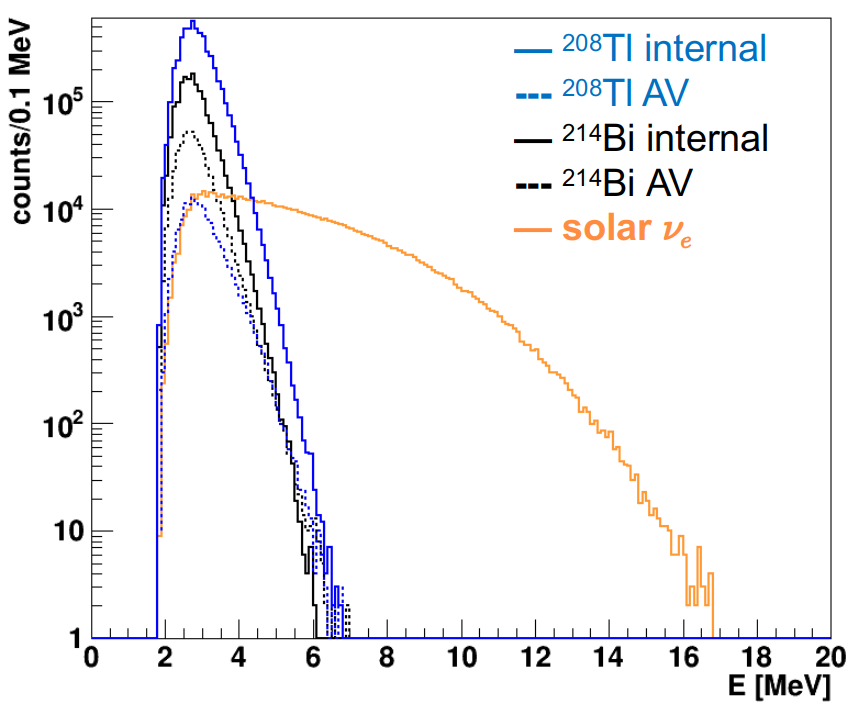
\includegraphics[width=8cm]{TMVA_bkgs_1.png}
	\caption[Energy spectrum of events from different simulations.]{Energy spectrum of events from different simulations in the half-dataset: $^{214}$Bi (black), $^{208}$Tl (blue) and solar $\nu_e$ (orange). Solid lines show the internal events and dotted lines show the AV events.}
	\label{TMVA_bkgs_1}
\end{figure}

From the simulations of the half-dataset, runs from run-200004 to 202516 were taken as the training set (about 67 live days and 72.4\% of the half-dataset), and the balance (run 202517 to 203602, 27.6\%) were taken as the testing set\footnote{For a more unbiased analysis, a bootstrap method \cite{murphy2012machine} that randomly separates the training and testing datasets can be used, but it was not applied here.}. The machine learning algorithms in the TMVA train the weights of the input variables by using the training set, while they apply the trained weights to the testing set for validations of the signal-background separation. Once the weights of the input variables were obtained, they were applied to the actual data. Three ranges of $E_{fit}$ were tested: $4<E_{fit}<15$ MeV, $5<E_{fit}<15$ MeV ($E>5$ MeV region), and $4<E_{fit}<5$ MeV (low energy region). Table.~\ref{tab:signalToBkg_tmva} lists the ratios of the signal event count ($N_{sig}$) to the background event count ($N_{bkg}$) for the different energy regions, after application of these beforehand cuts. In the low energy region $4<E_{fit}<5$ MeV background events are dominant, while for  $E_{fit}>5$ MeV background events are significantly reduced.

\begin{table}[ht]
	\centering
	\caption{Ratios of the signal event numbers to the background event numbers.}
	\label{tab:signalToBkg_tmva}
	\begin{tabular*}{100mm}{c@{\extracolsep{\fill}}ccc}
		\toprule
		energy region (MeV) & $N_{sig}$ & $N_{bkg}$ & $N_{sig}/N_{bkg}$ \\
		\midrule
		$4<E_{fit}<15$ & 434830& 166280& 2.6 \\ 
		\midrule
		$5<E_{fit}<15$ & 317205 & 6359 & 49.9\\
		\midrule
		$4<E_{fit}<5$ & 117625 & 159921& 0.73\\
		\bottomrule
	\end{tabular*}
\end{table}

Three machine-learning algorithms/classification methods implemented in the \texttt{TMVA} package were applied to the training and testing datasets: the Fisher discriminants/linear discriminant analysis (Fisher/LD), the Boosted Decision Tree (BDT), and the Artificial Neural Networks Multilayer Perceptron (ANN-MLP, or MLP in short) \cite{albertsson2007tmva}.

The Fisher discriminant $y_{F_i}(i)$ for classifying event $i$ is defined by \cite{tmvaWebsite}:
\begin{equation}
y_{F_i}(i) = F_0+\sum_{k=1}^{n_{params}}F_k x_k(i),
\end{equation}
where $n_{params}$ is the number of input variables, and the Fisher coefficient $F_k$ is given by:
\begin{equation}
F_k = \frac{\sqrt{N_SN_B}}{N_S+N_B}\sum_{l=1}^{n_{params}}1/W_{kl}(\bar{x}_{S,l}-\bar{x}_{B,l}),
\end{equation} 
where $N_{S(B)}$ are the number of signal (background) events in the training sample; $\bar{x}_{{S(B),l}}$ are the means of input variables for signal (background); and $W_{kl}$ is the covariance matrix \cite{tmvaWebsite}.

For the settings in the TMVA, the BDT method was set by: (1) using the adaptive boosting (AdaBoost) algorithm; (2) training 400 trees with a maximum depth of 3; and (3) using gini index for the decision tree. 

The MLP method was set with: (1) using sigmoid function as the activate function; and (2) using neural networks with 4 hidden layers and 200 training cycles.

Nine variables were used as the TMVA inputs: ITR, $\beta_{14}$, $E_{fit}$, $G_{test}$, $U_{test}$, $scaleLogL$, $Z_{factor}$, $\vec{u}\cdot \vec{R}$ and $klDiv$ (in the symmetrical form: Eqn.~\ref{eq:symKlDiv}). Among them, the beforehand cuts had been applied to the ITR and $\beta_{14}$, and the $E_{fit}$ had been selected for different regions, as mentioned previously. NHits and $\theta_{ij}$ were not used for they are considered redundant:  NHits is correlated with the event energy, while $\theta_{ij}$ is anticorrelated with $\beta_{14}$. 

Using the $4<E<15$ MeV training dataset as an example, the distributions of these variables are shown in Fig.~\ref{fig:inputParamsTMVA}. The differences in distributions between the signal inputs (black solid lines) and background inputs (red dotted lines) can be observed.

\begin{figure}[htbp]
	\centering
	\subfigure[$\beta_{14}$]{
		\begin{minipage}[t]{0.3\textwidth}
			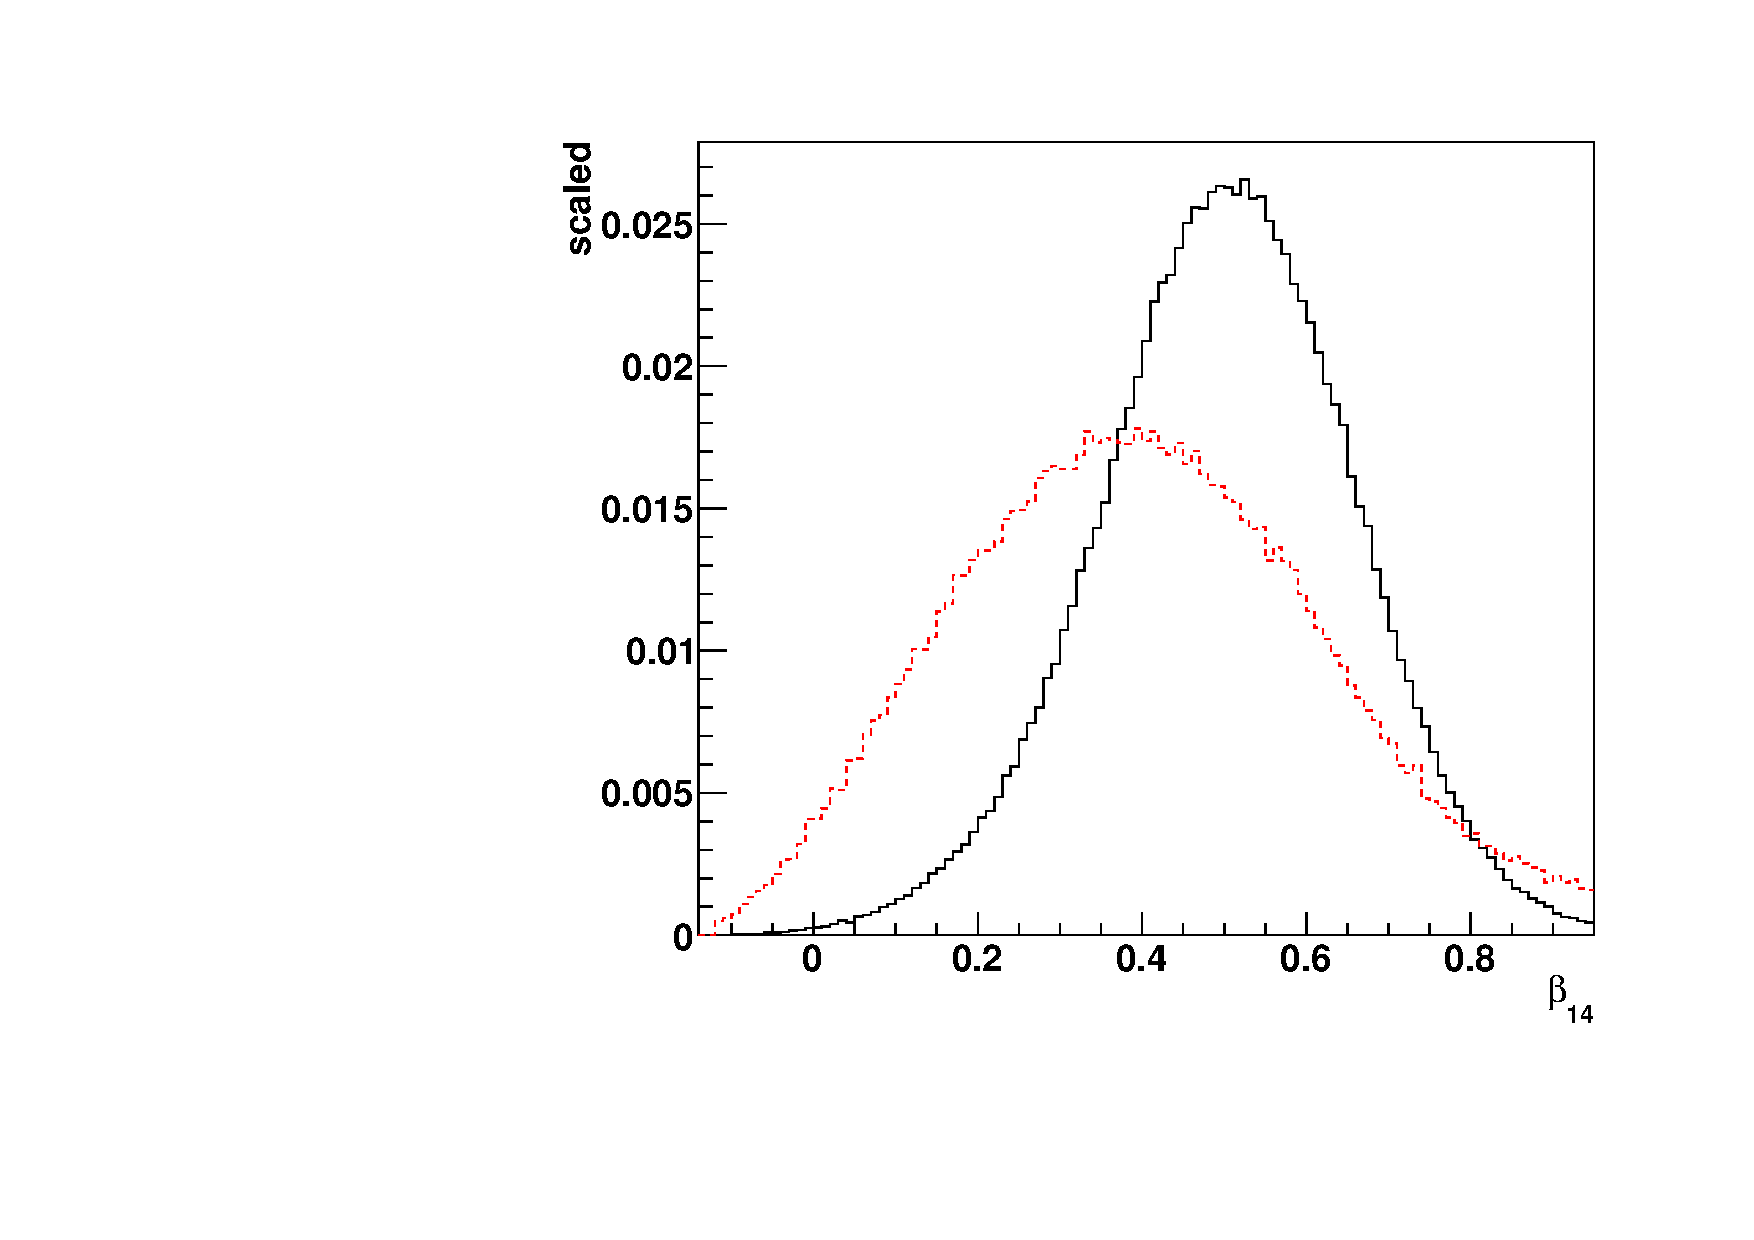
\includegraphics[width=4cm]{tmvaCompare_Beta14.pdf}
		\end{minipage}
	}
	\subfigure[$E_{fit}$]{
		\begin{minipage}[b]{0.3\textwidth}
			\centering
			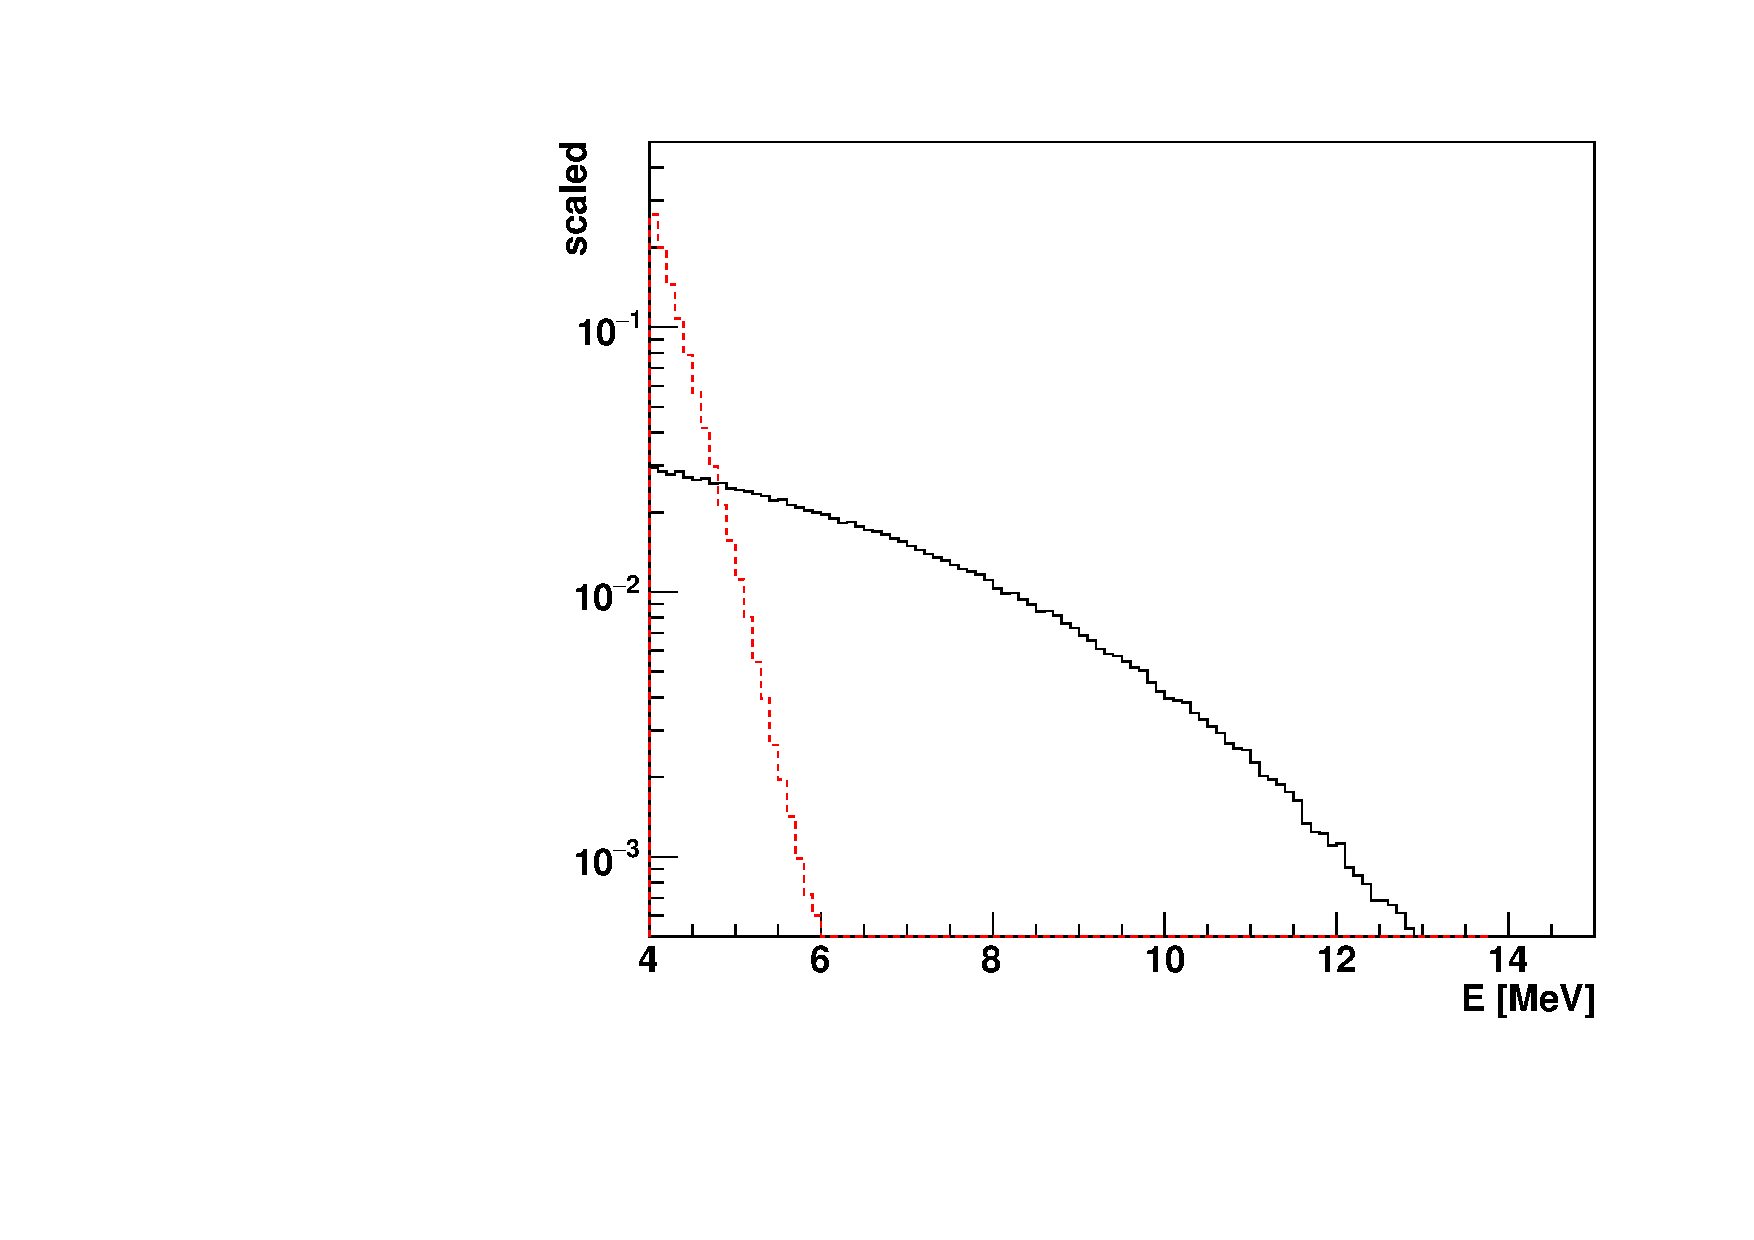
\includegraphics[width=4cm]{tmvaCompare_energy.pdf}
		\end{minipage}
	}
	\subfigure[$G_{test}$]{
		\begin{minipage}[b]{0.3\textwidth}
			\centering
			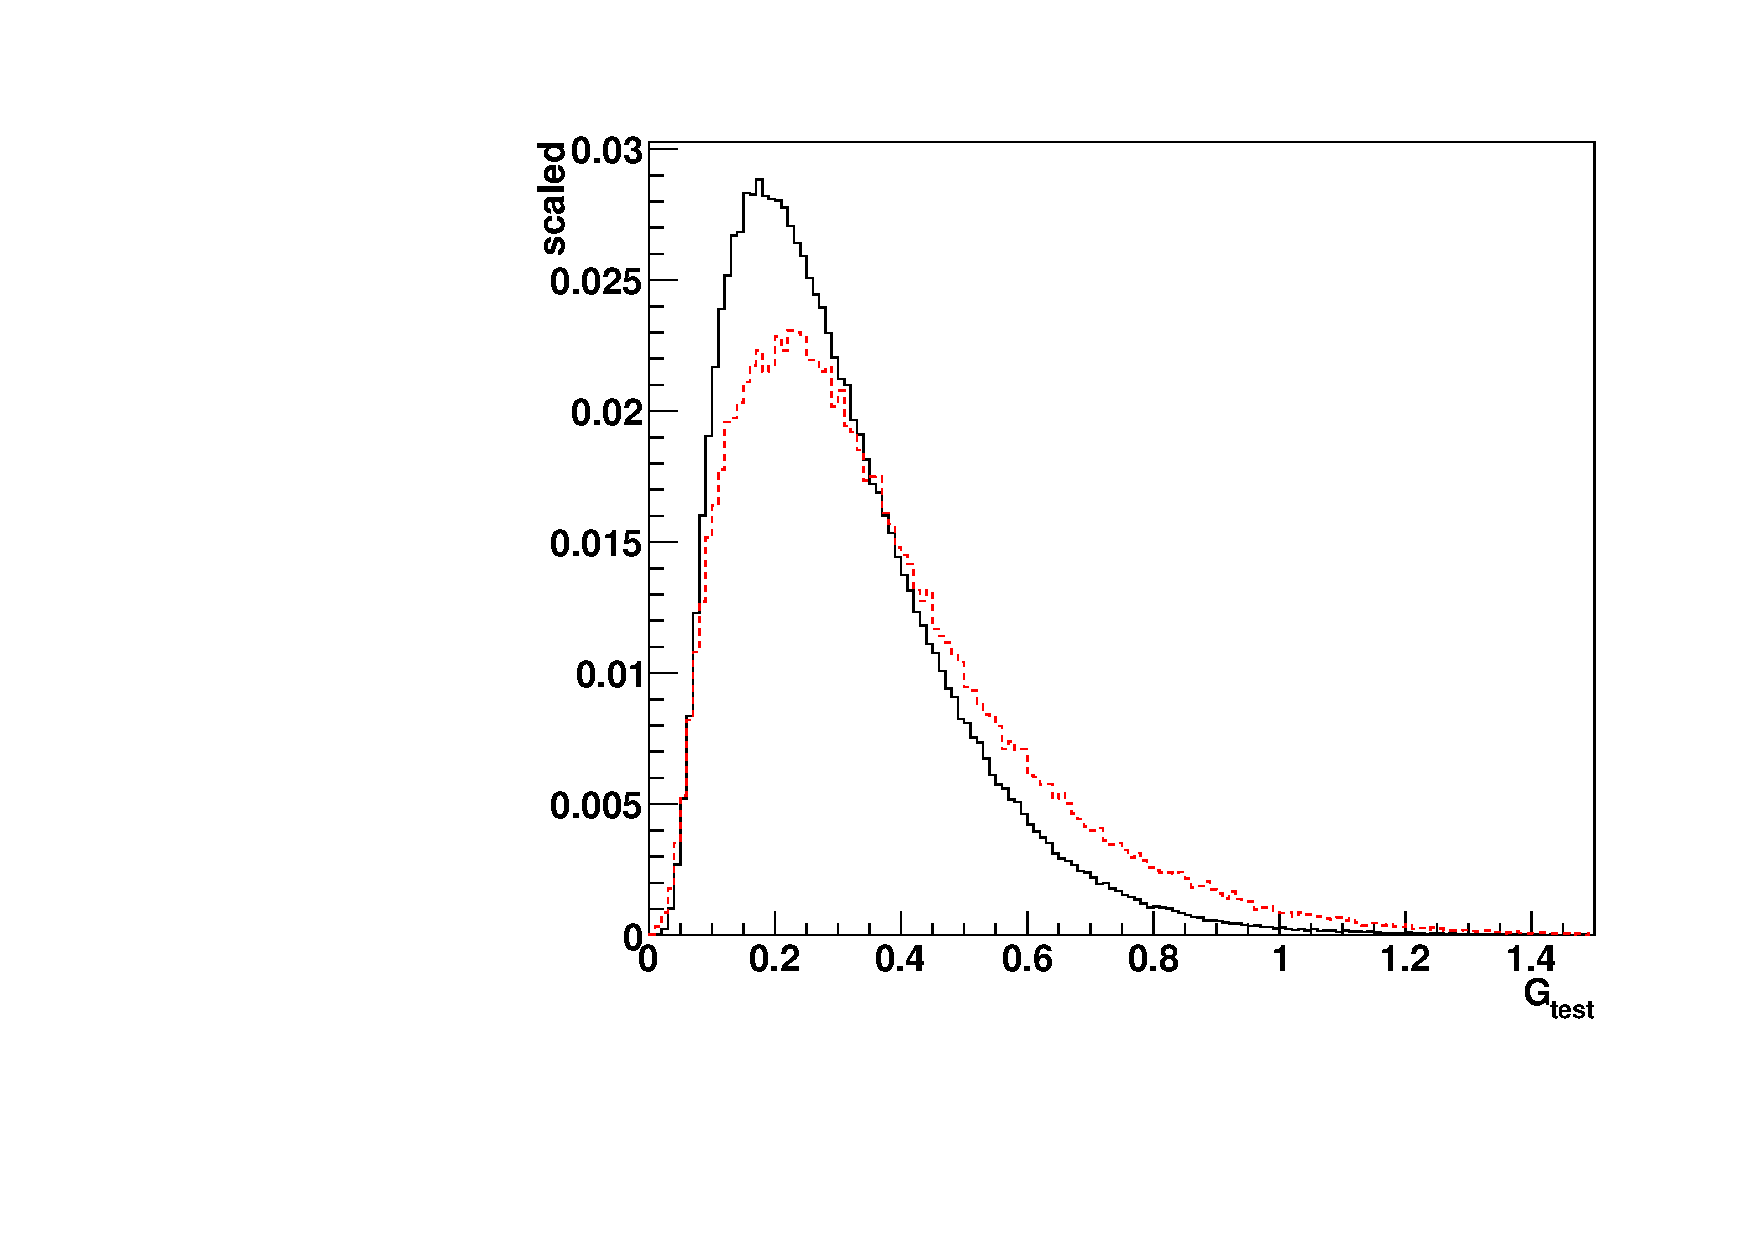
\includegraphics[width=4cm]{tmvaCompare_Gtest.pdf}
		\end{minipage}
	}
	\subfigure[$U_{test}$]{
		\begin{minipage}[b]{0.3\textwidth}
			\centering
			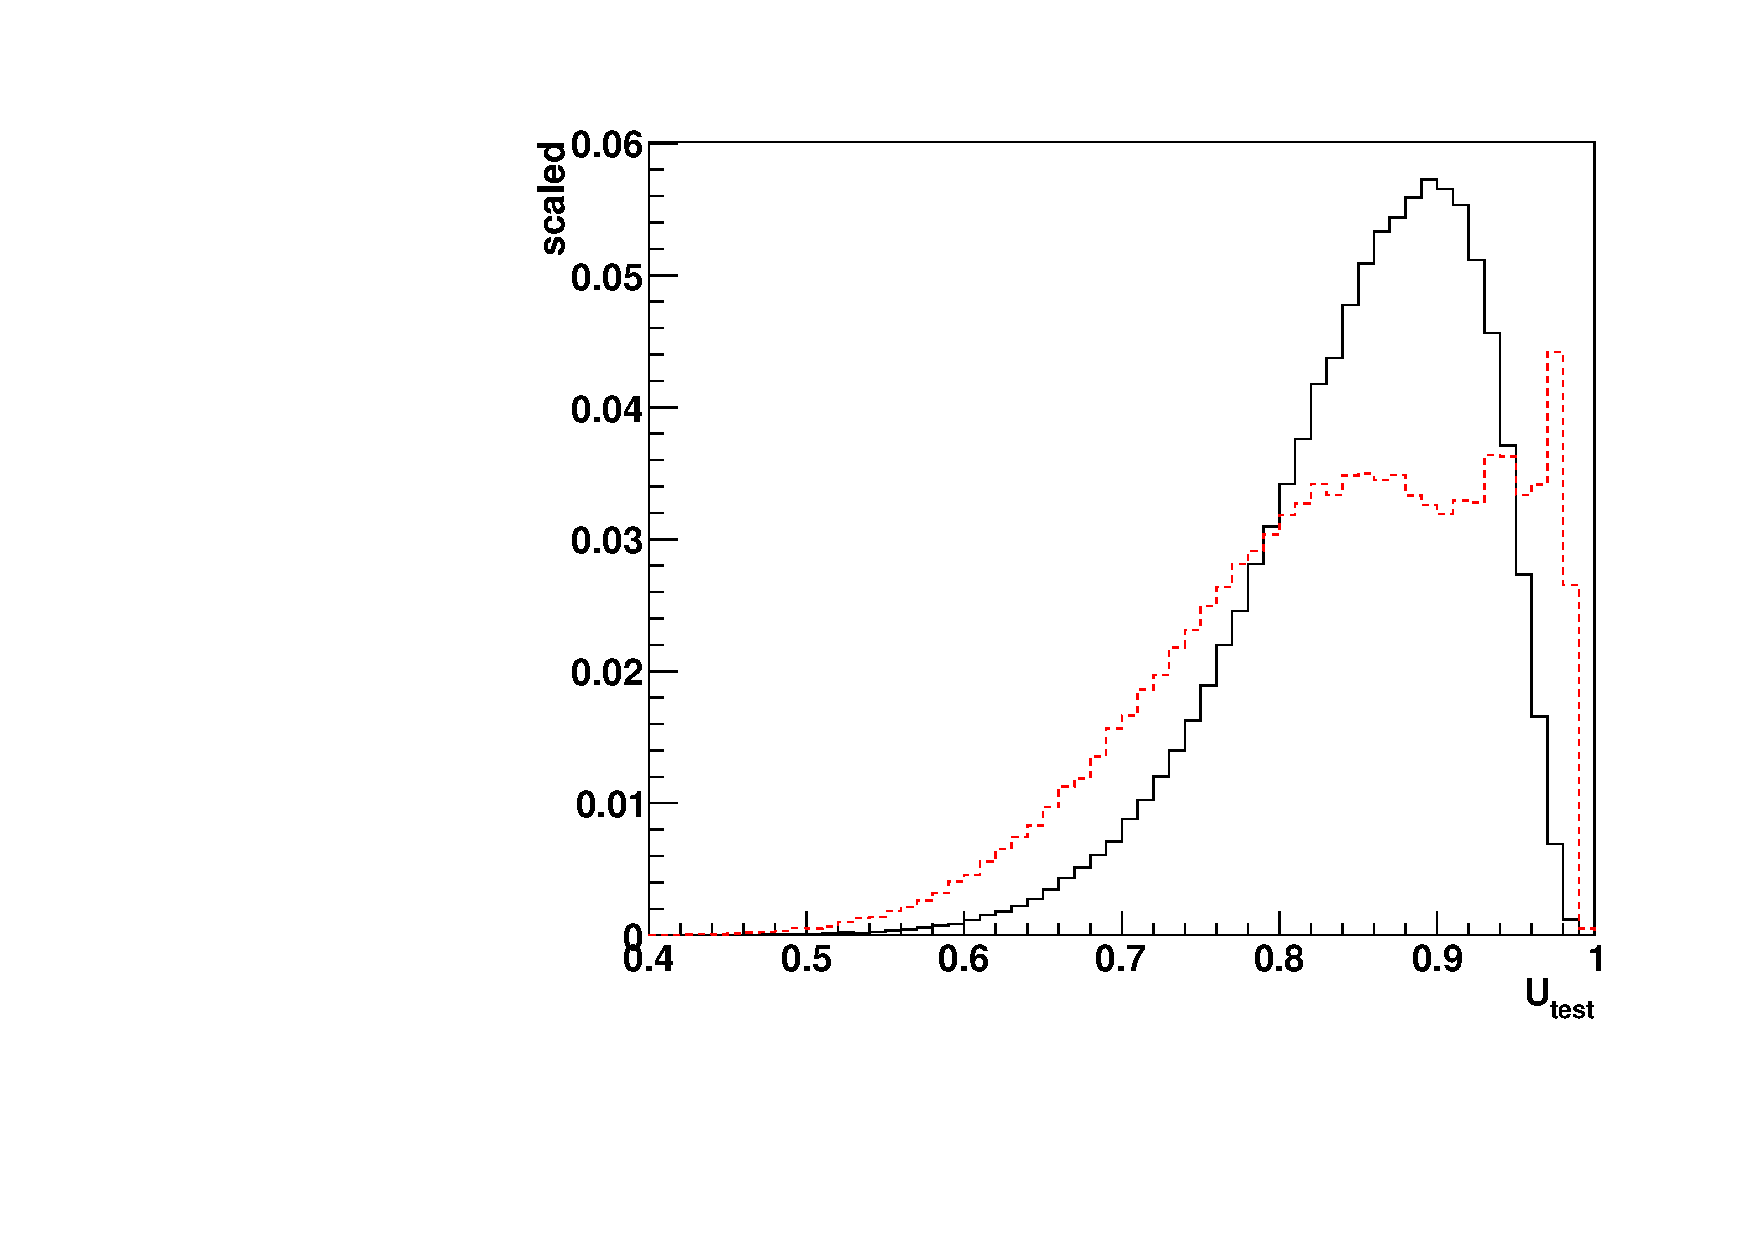
\includegraphics[width=4cm]{tmvaCompare_Utest.pdf}
		\end{minipage}
	}	
	\subfigure[$Z_{factor}$]{
		\begin{minipage}[b]{0.3\textwidth}
			\centering
			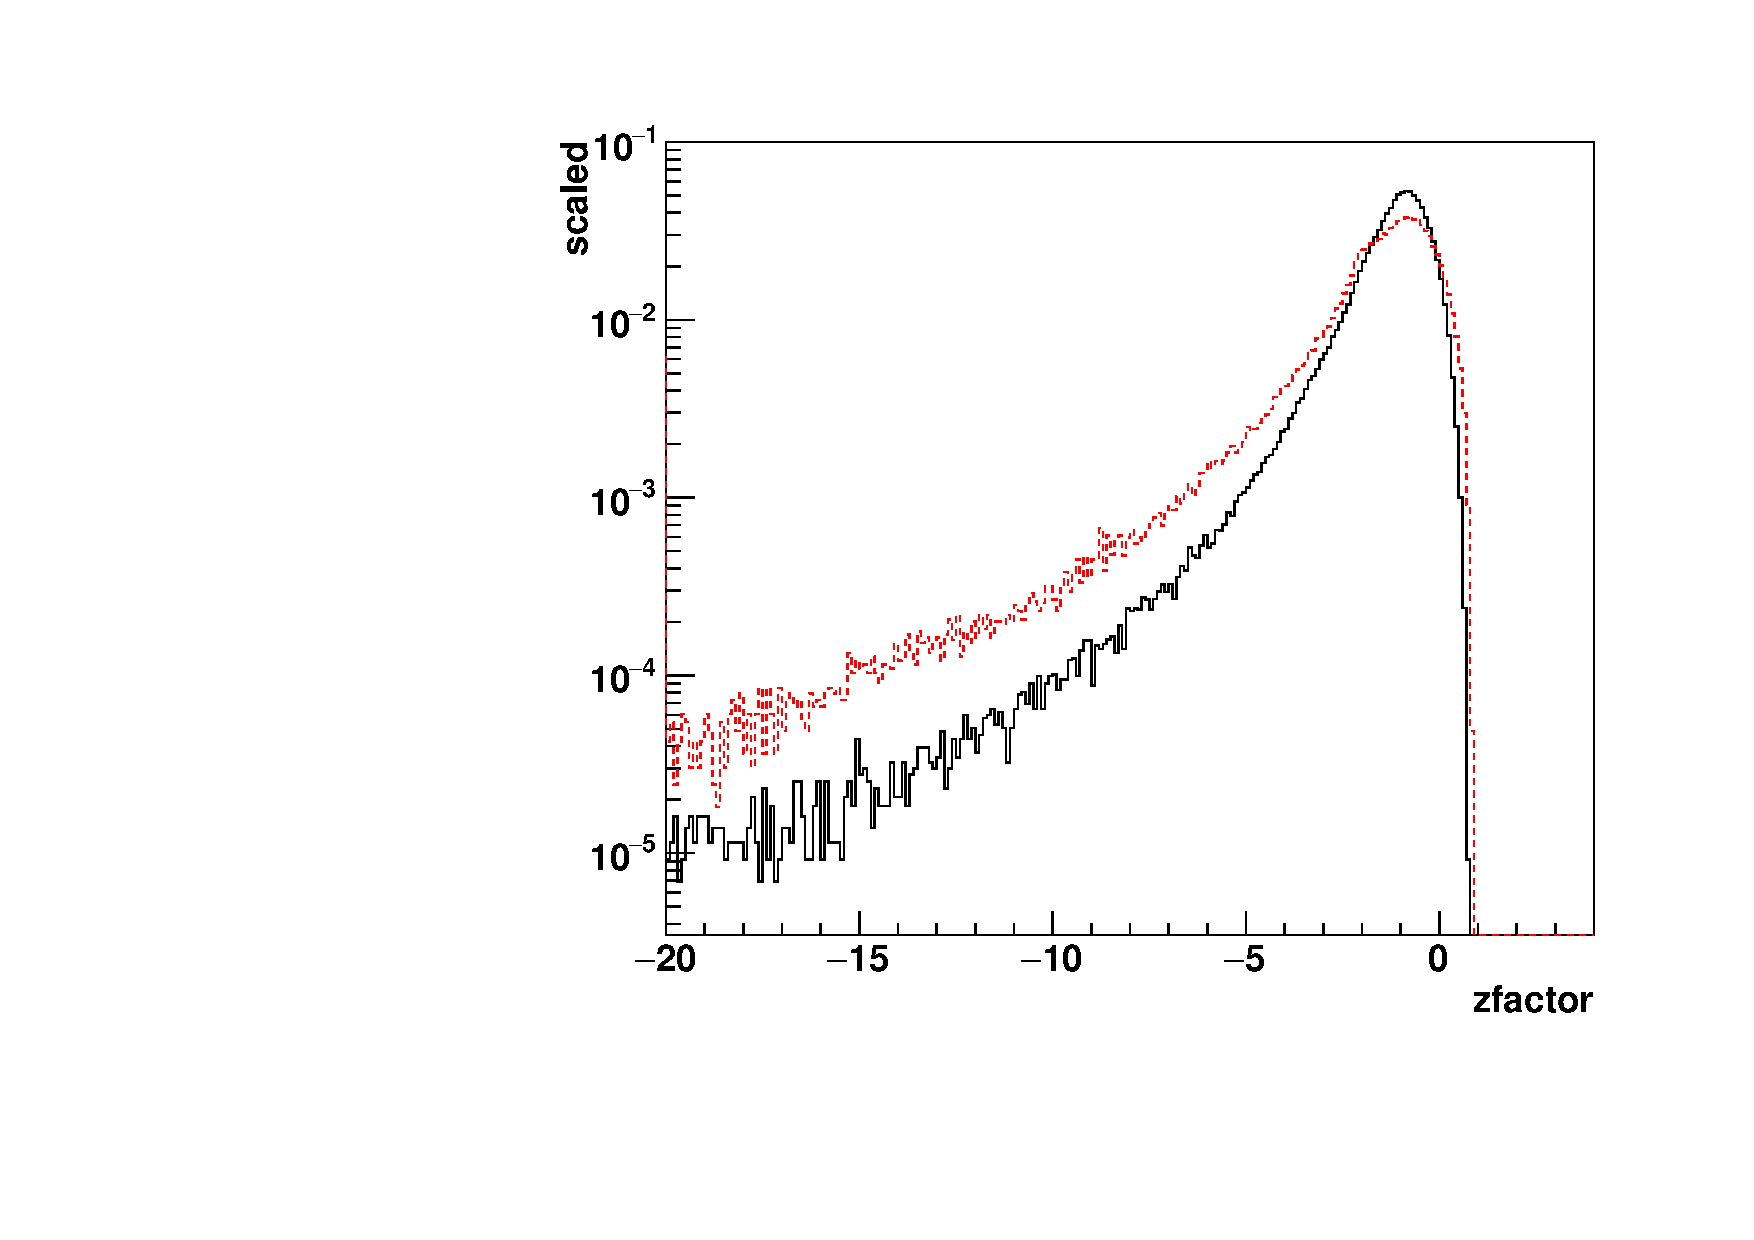
\includegraphics[width=4cm]{tmvaCompare_zfactor.pdf}
		\end{minipage}
	}	
	\subfigure[ITR]{
		\begin{minipage}[b]{0.3\textwidth}
			\centering
			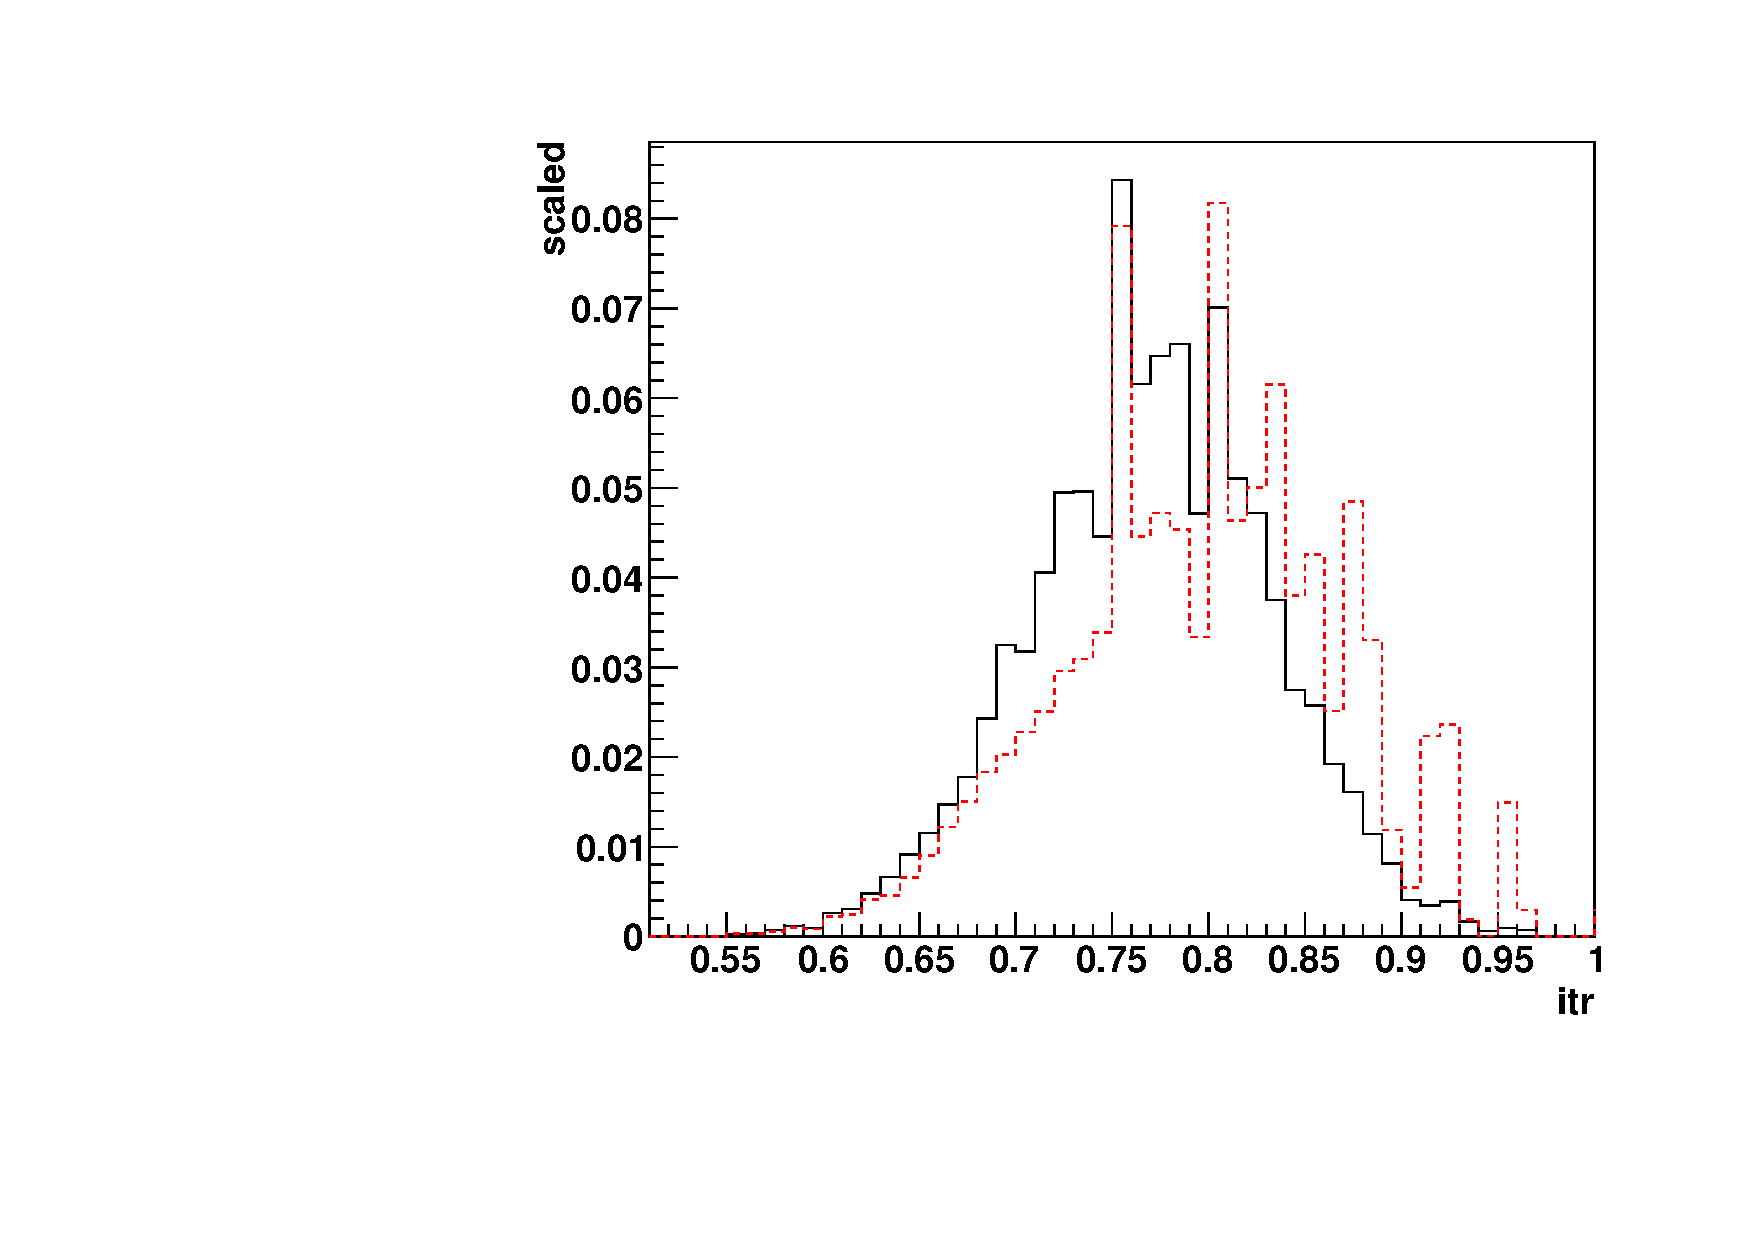
\includegraphics[width=4cm]{tmvaCompare_itr.pdf}
		\end{minipage}
	}	
	\subfigure[$\vec{u}\cdot\vec{R'}$]{
		\begin{minipage}[b]{0.3\textwidth}
			\centering
			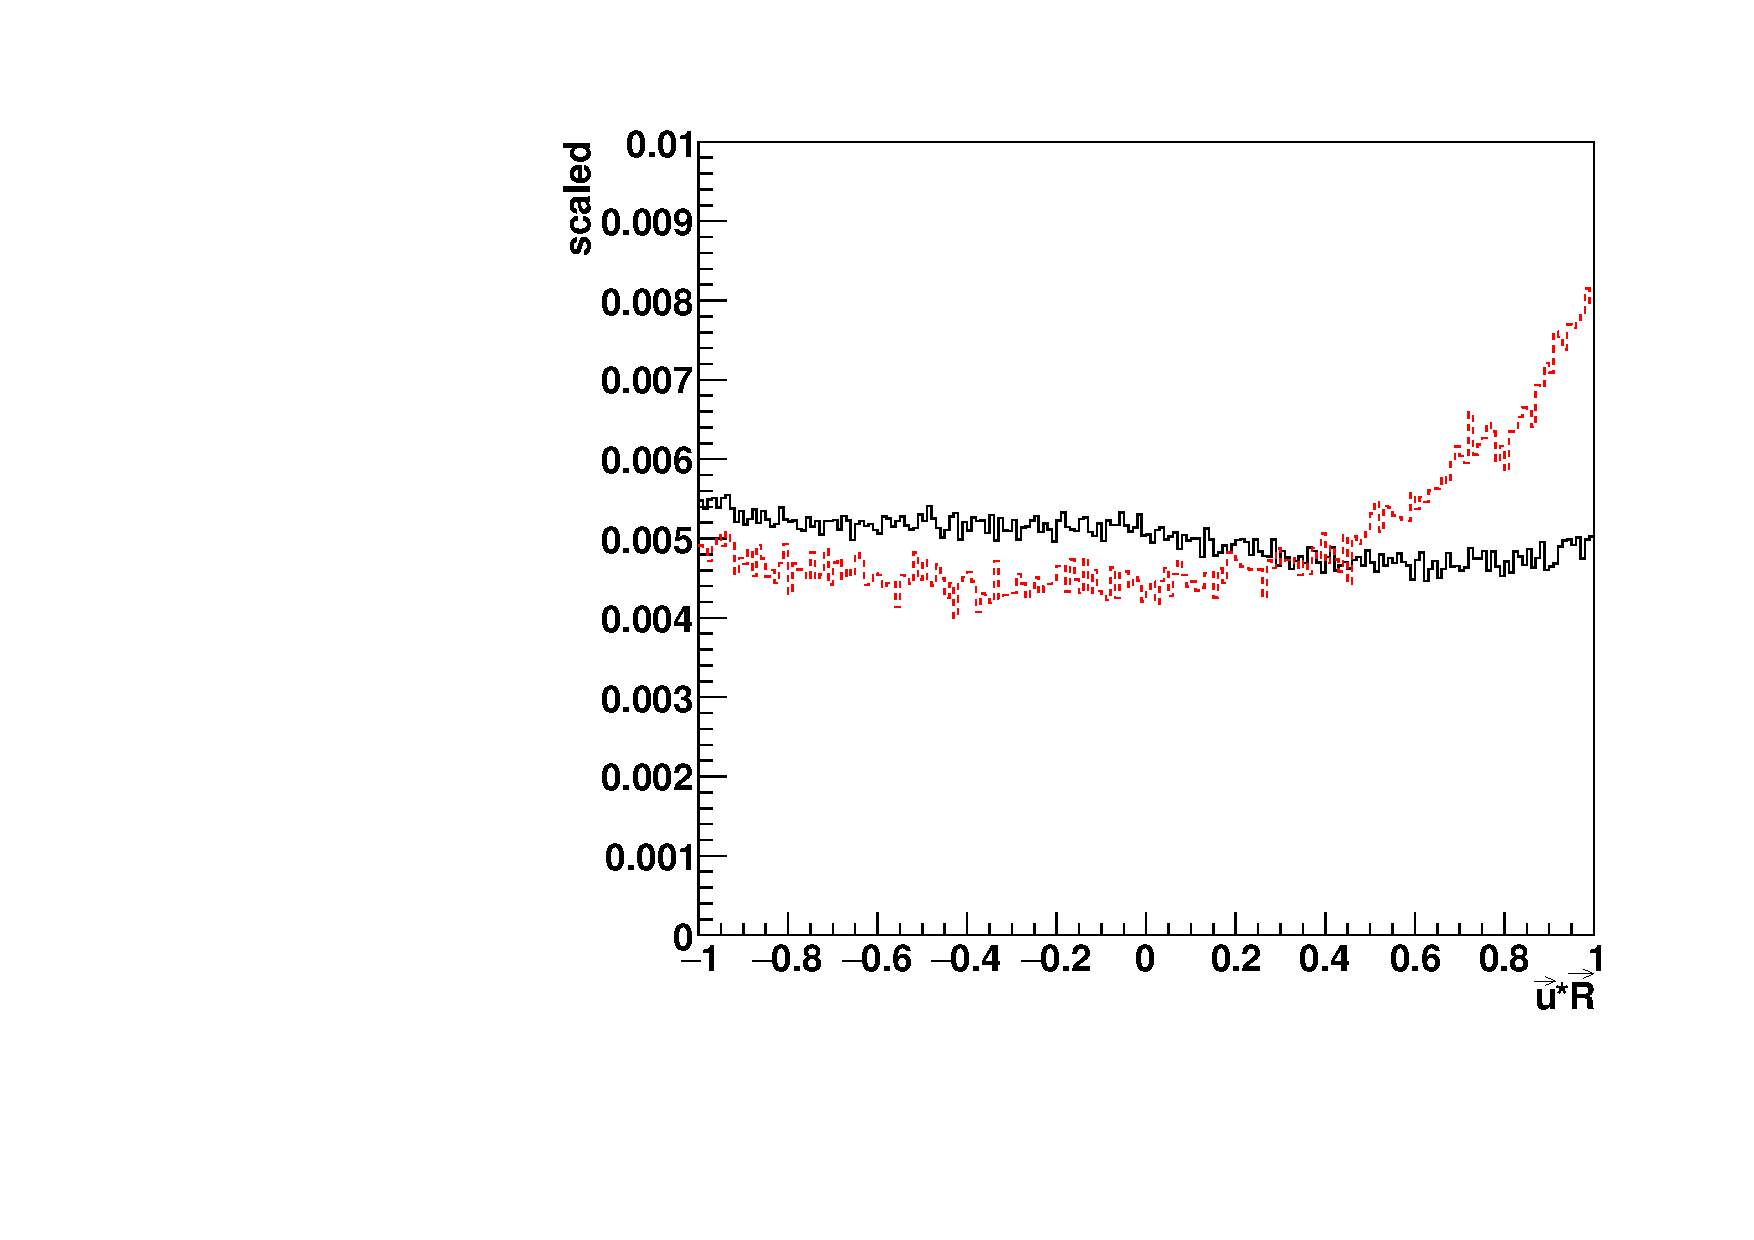
\includegraphics[width=4cm]{tmvaCompare_udotR.pdf}
		\end{minipage}
	}
	\subfigure[$scaleLogL$]{
		\begin{minipage}[b]{0.3\textwidth}
			\centering
			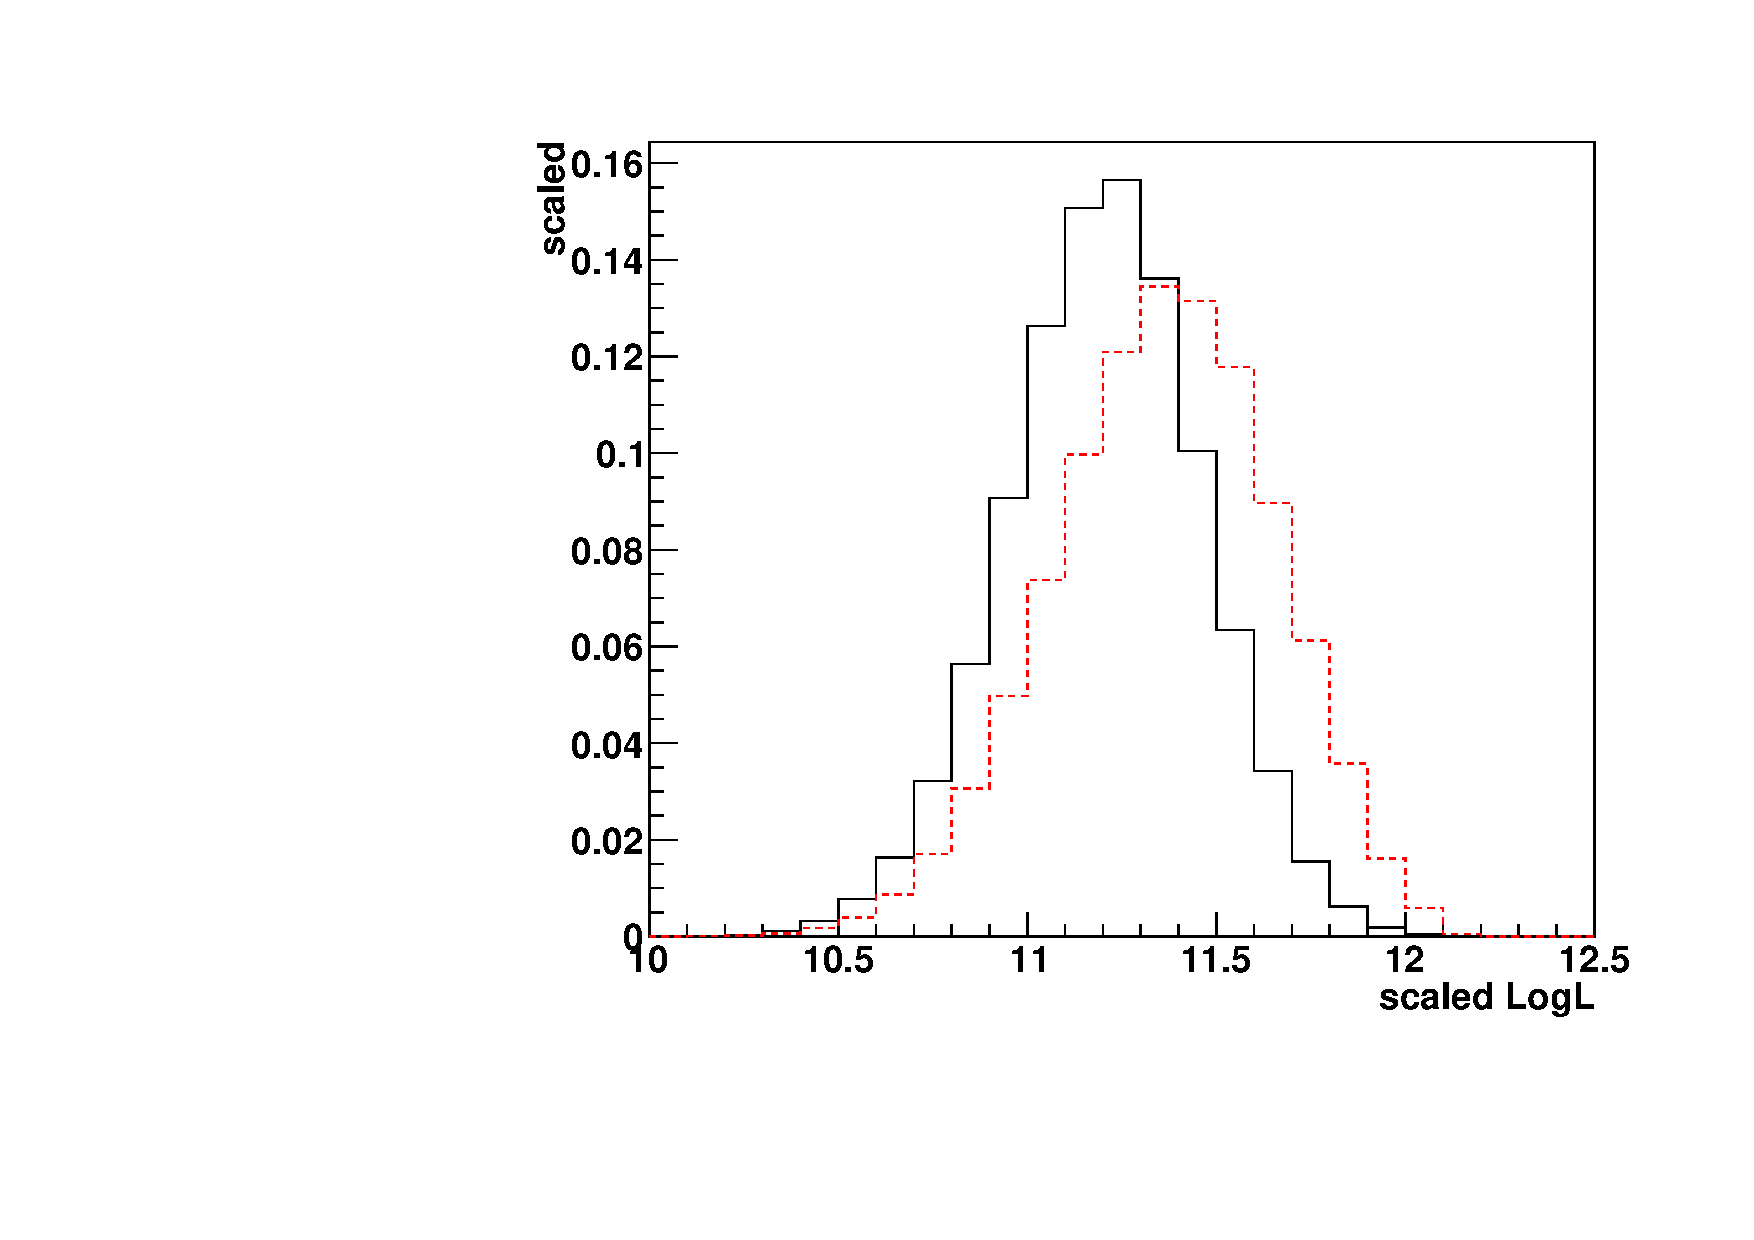
\includegraphics[width=4cm]{tmvaCompare_scaleLogL.pdf}
		\end{minipage}
	}	
	\subfigure[$klDiv$]{
		\begin{minipage}[b]{0.3\textwidth}
			\centering
			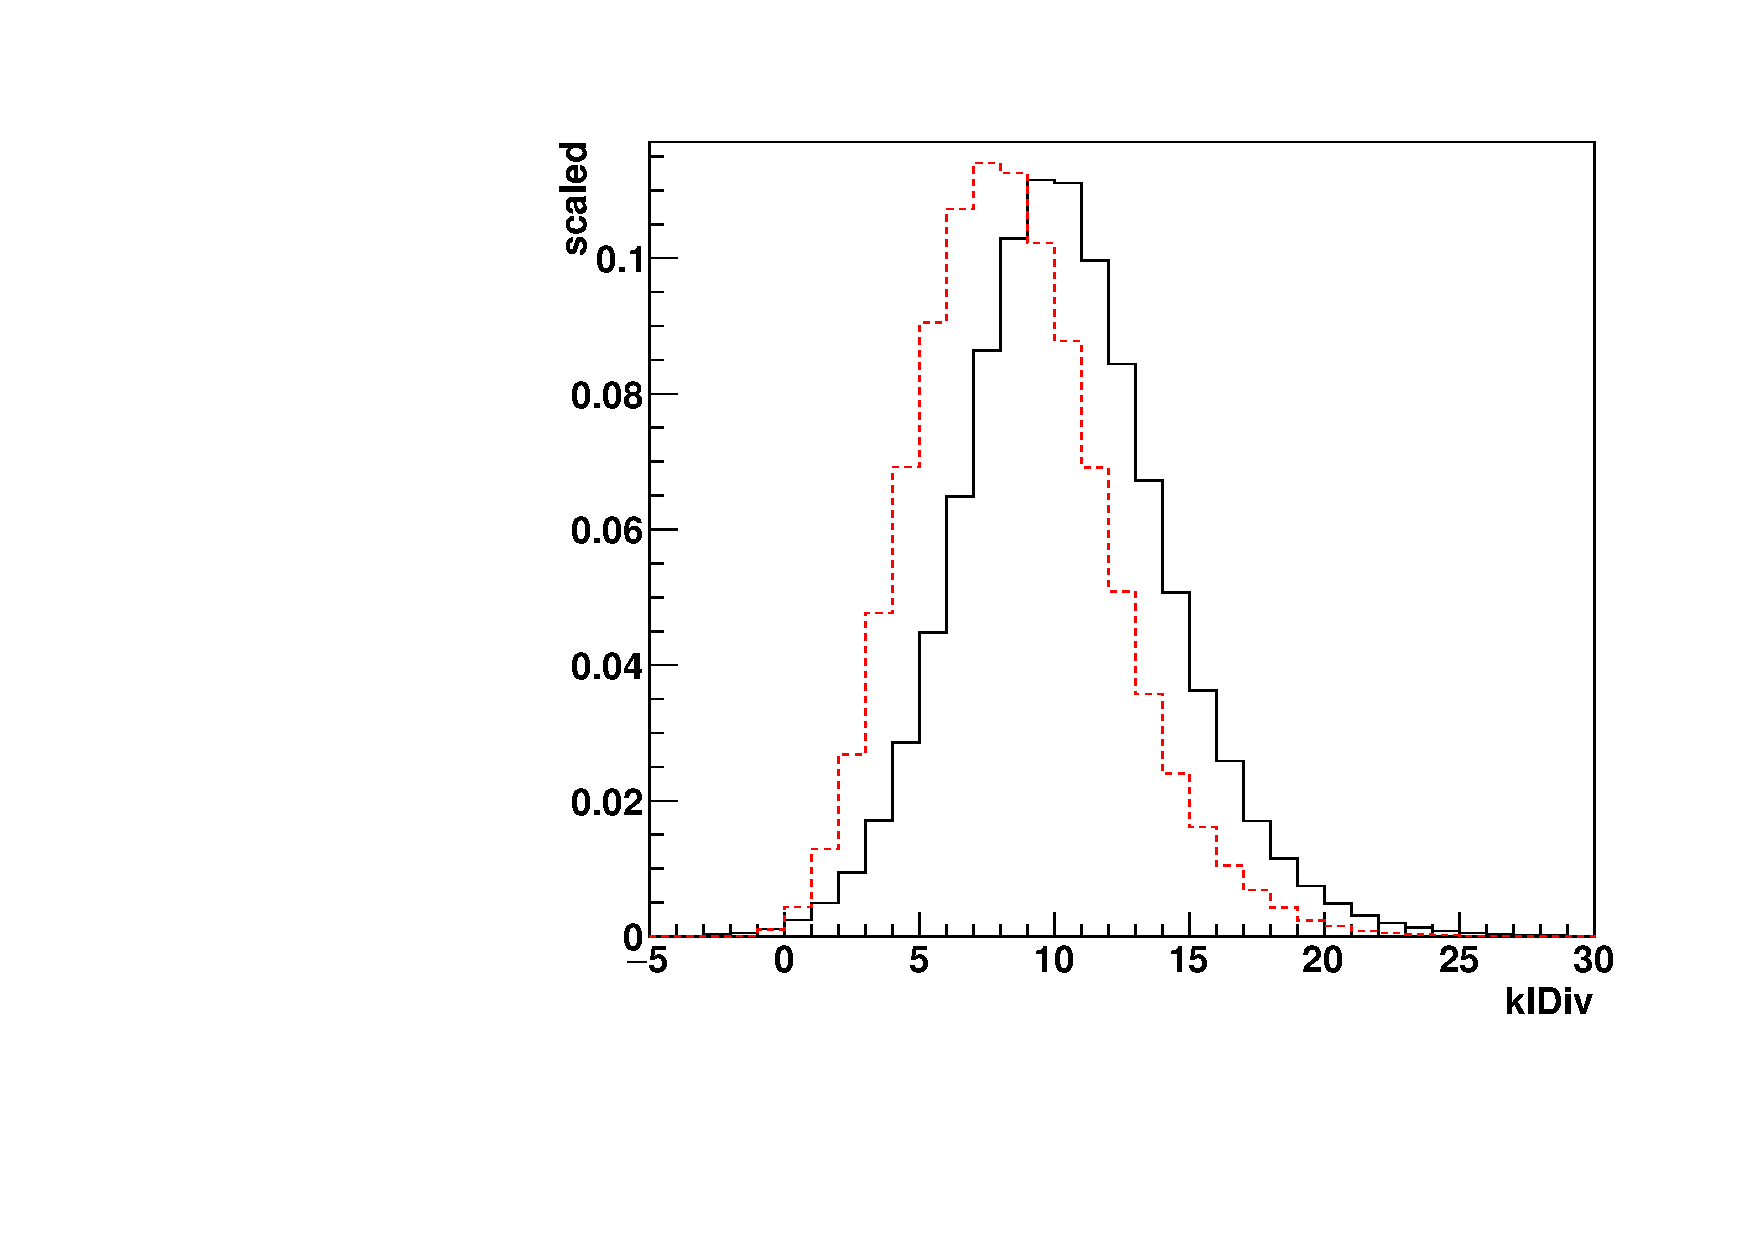
\includegraphics[width=4cm]{tmvaCompare_klDiv.pdf}
		\end{minipage}
	}
	%   \subfigure[$\cos\theta_\mathrm{sun}$]{
	%	\begin{minipage}[b]{0.3\textwidth}
	%		\centering
	%		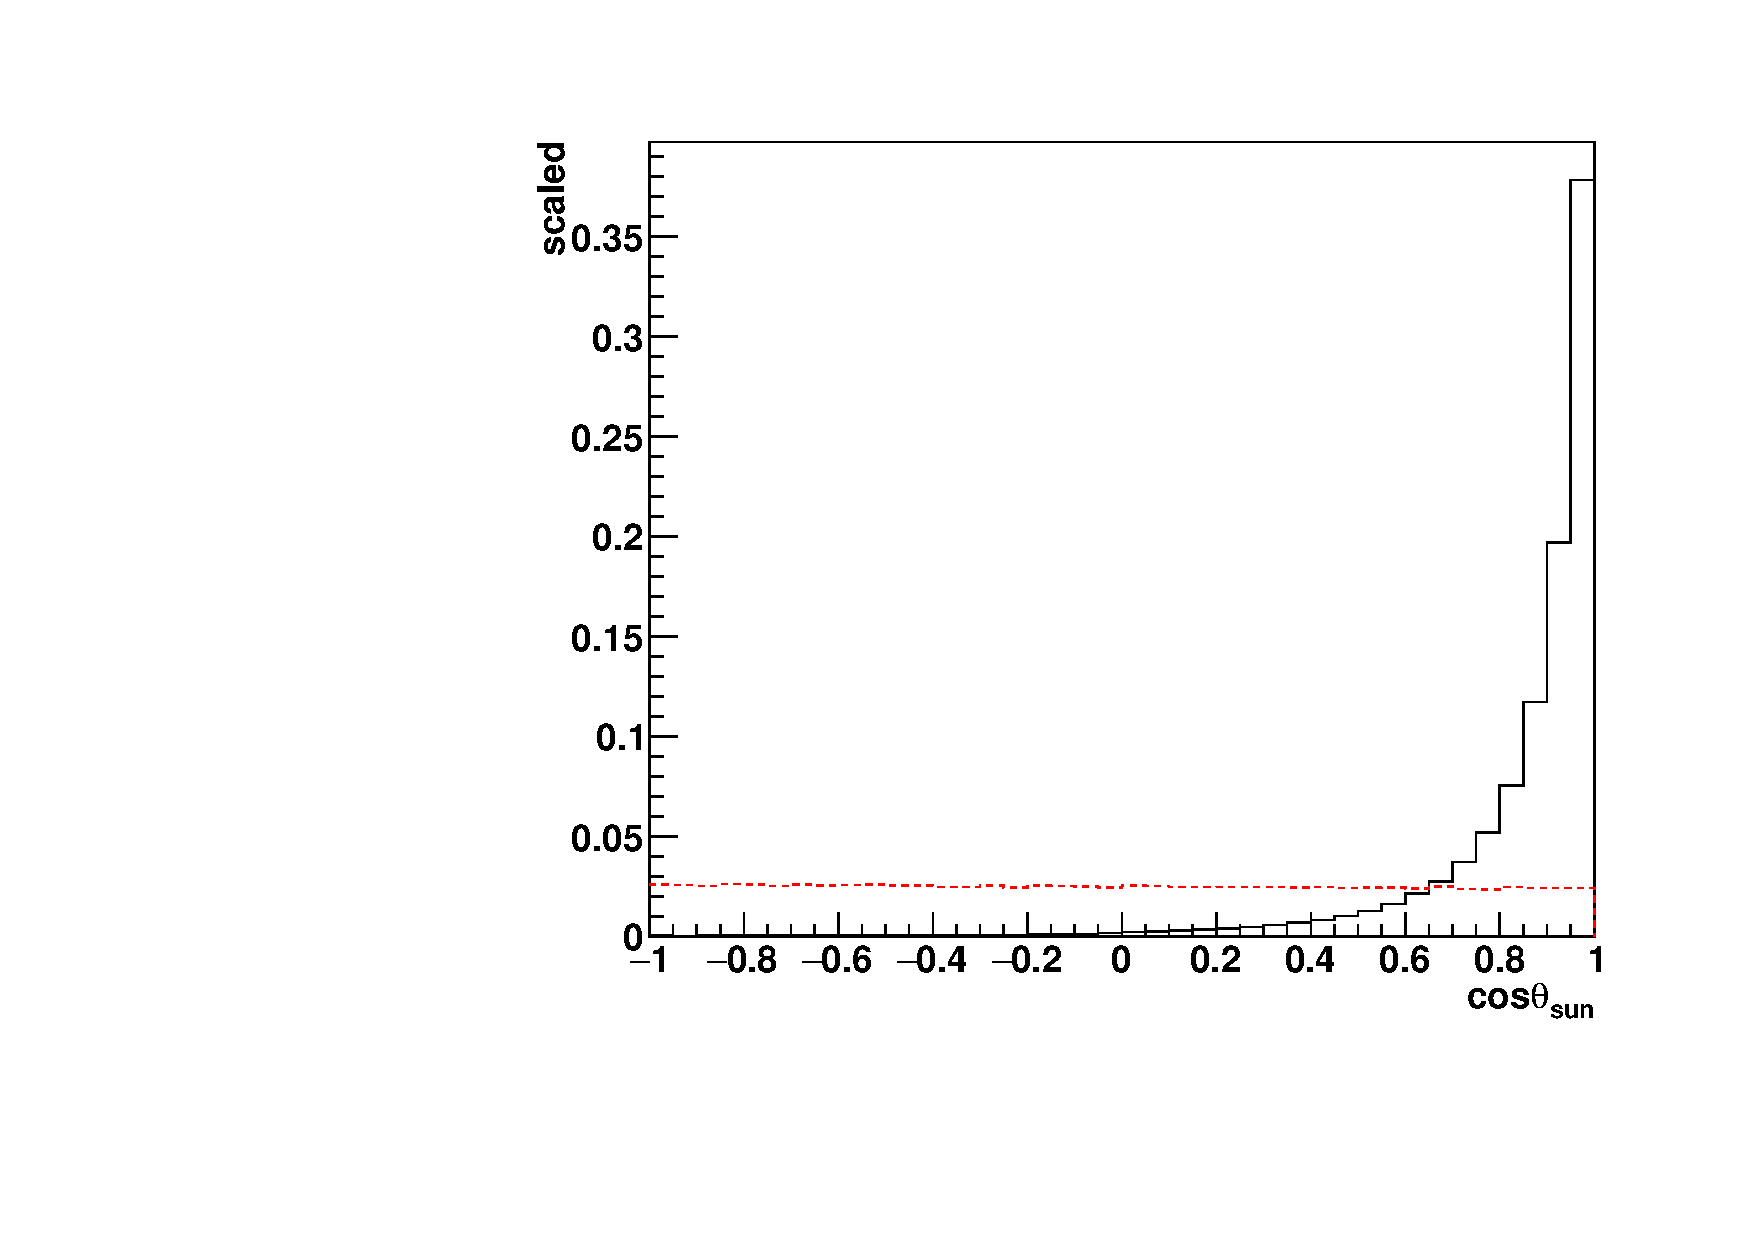
\includegraphics[width=4cm]{tmvaCompare_cosThetaSun.pdf}
	%	\end{minipage}
	%   }	
	\caption[Multiple variables as the inputs for the TMVA analysis, for the $4<E<15$ MeV dataset.]{Multiple variables as the inputs for the TMVA analysis, for the $4<E<15$ MeV dataset. The distributions of the backgrounds are show in dotted red lines while the signals are shown in solid black lines. The distributions are normalized to their integrals.\label{fig:inputParamsTMVA}}
\end{figure}

The output signal/background distributions on the test sub-dataset are shown in Fig.~\ref{output_separation_allE}.
\begin{figure}[htbp]
	\centering
	\subfigure[Fisher/LD output.]{
		\begin{minipage}[t]{0.5\textwidth}
			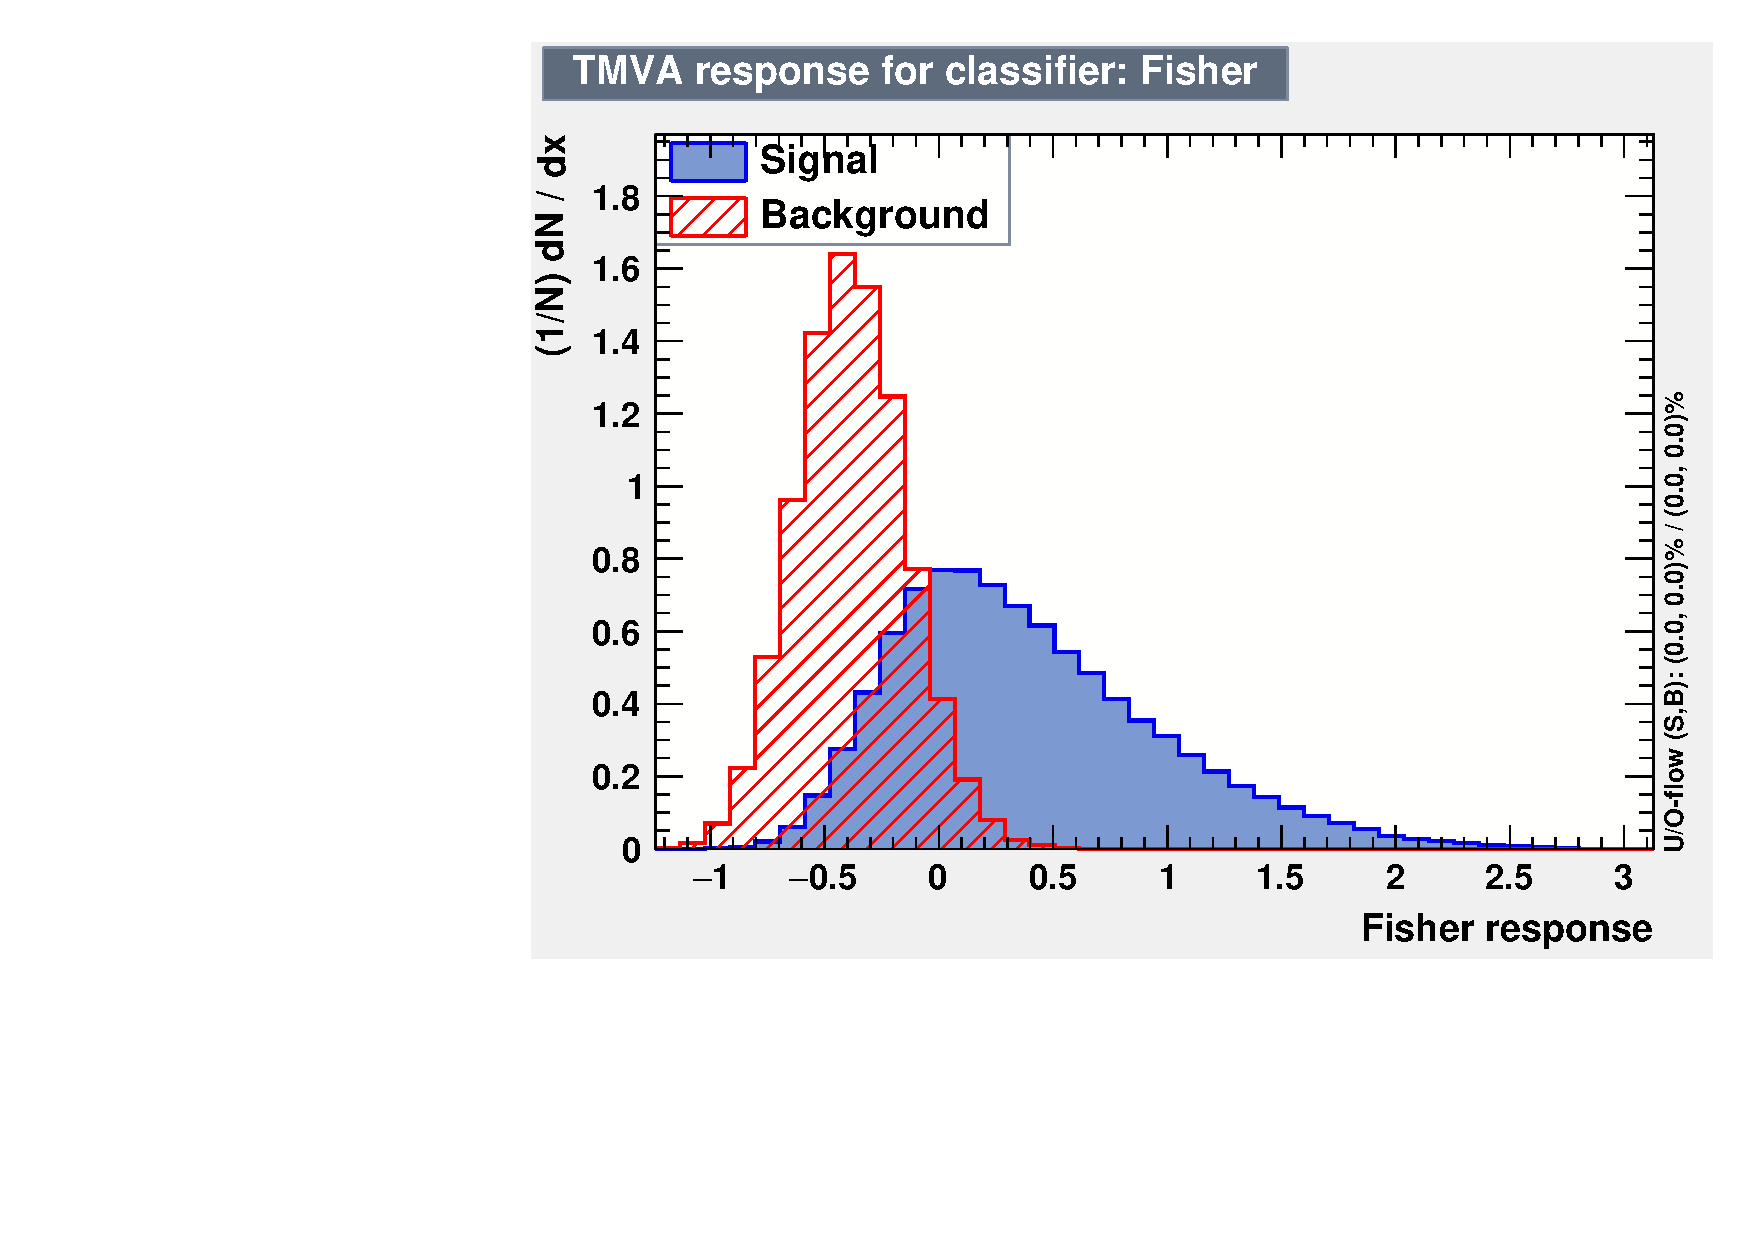
\includegraphics[width=8cm]{output_allE_Fisher.pdf}
		\end{minipage}
	}
	\subfigure[BDT output.]{
		\begin{minipage}[b]{0.4\textwidth}
			\centering
			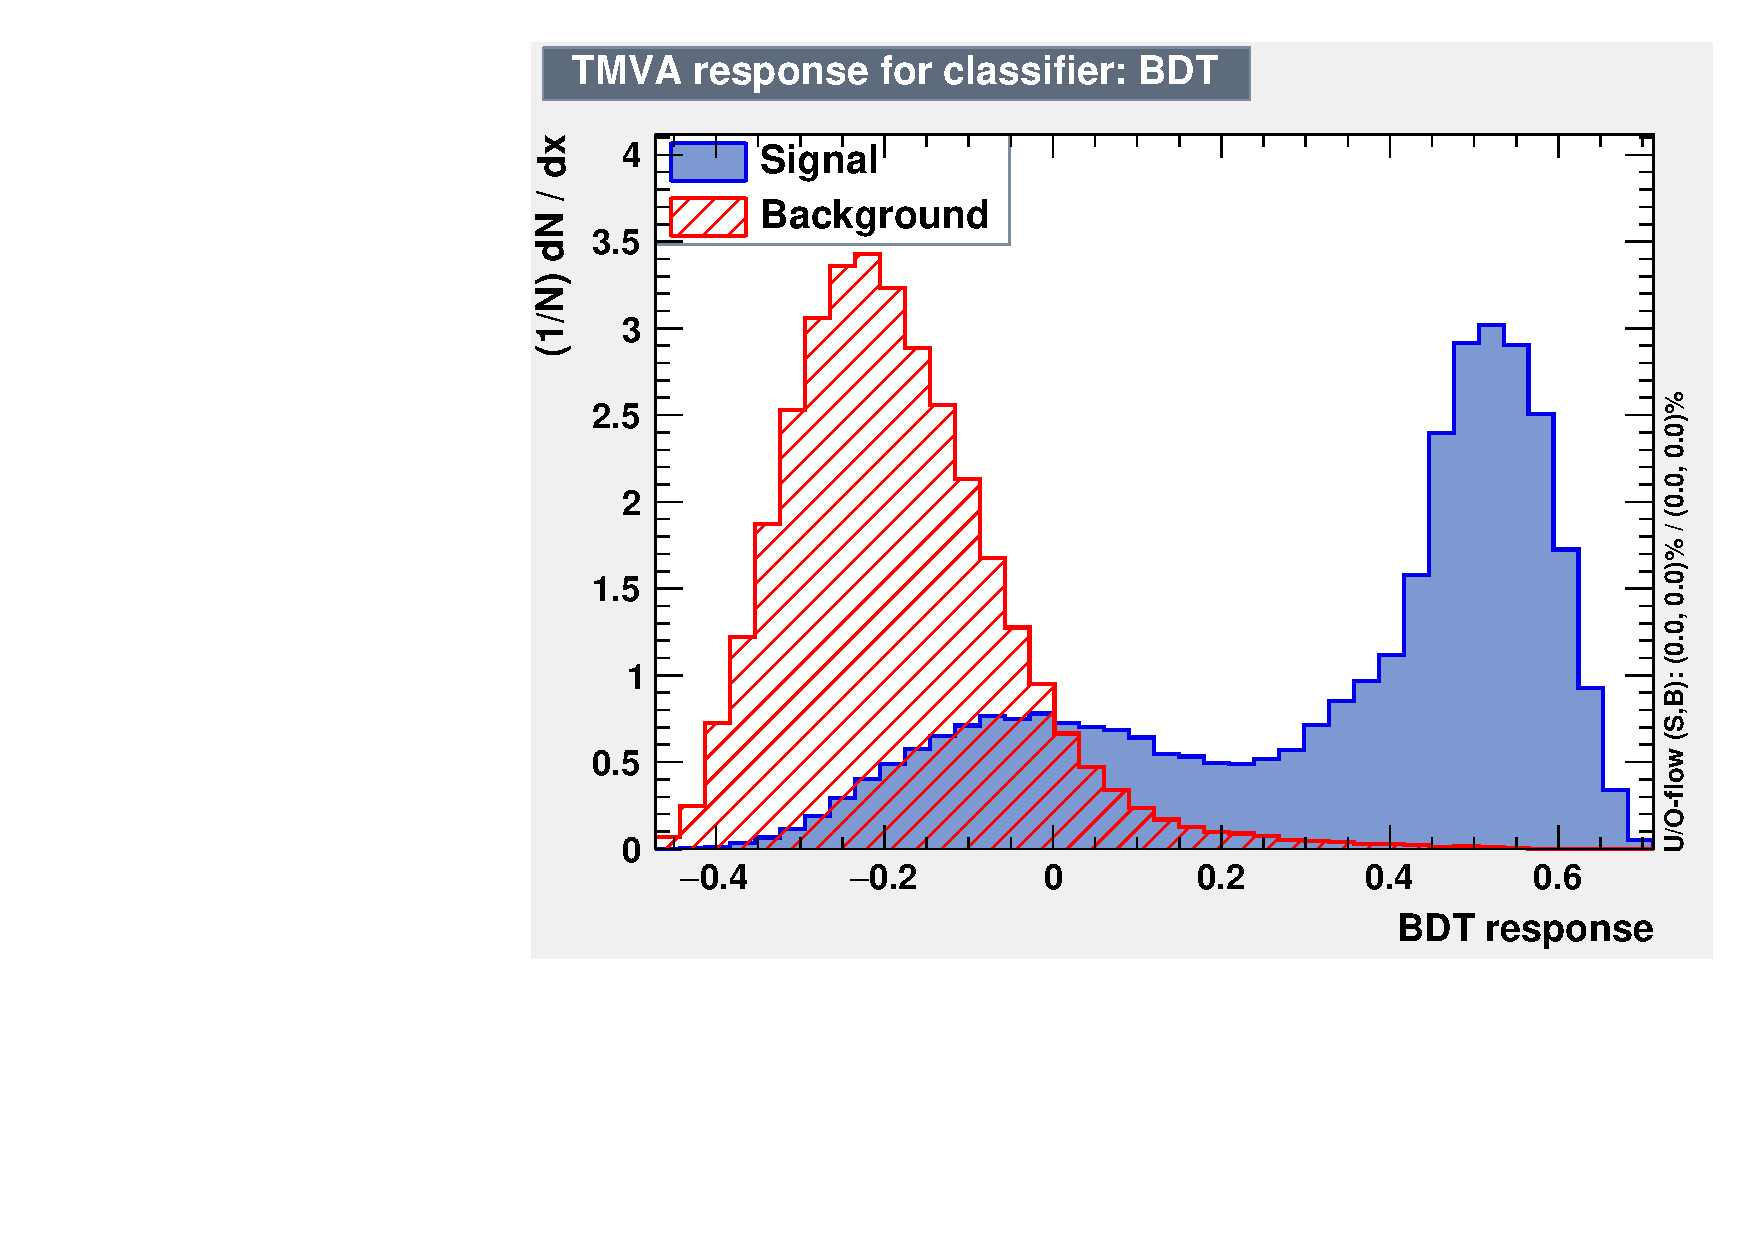
\includegraphics[width=8cm]{output_allE_BDT.pdf}
		\end{minipage}
	}
	\subfigure[MLP output]{
		\begin{minipage}[b]{0.4\textwidth}
			\centering
			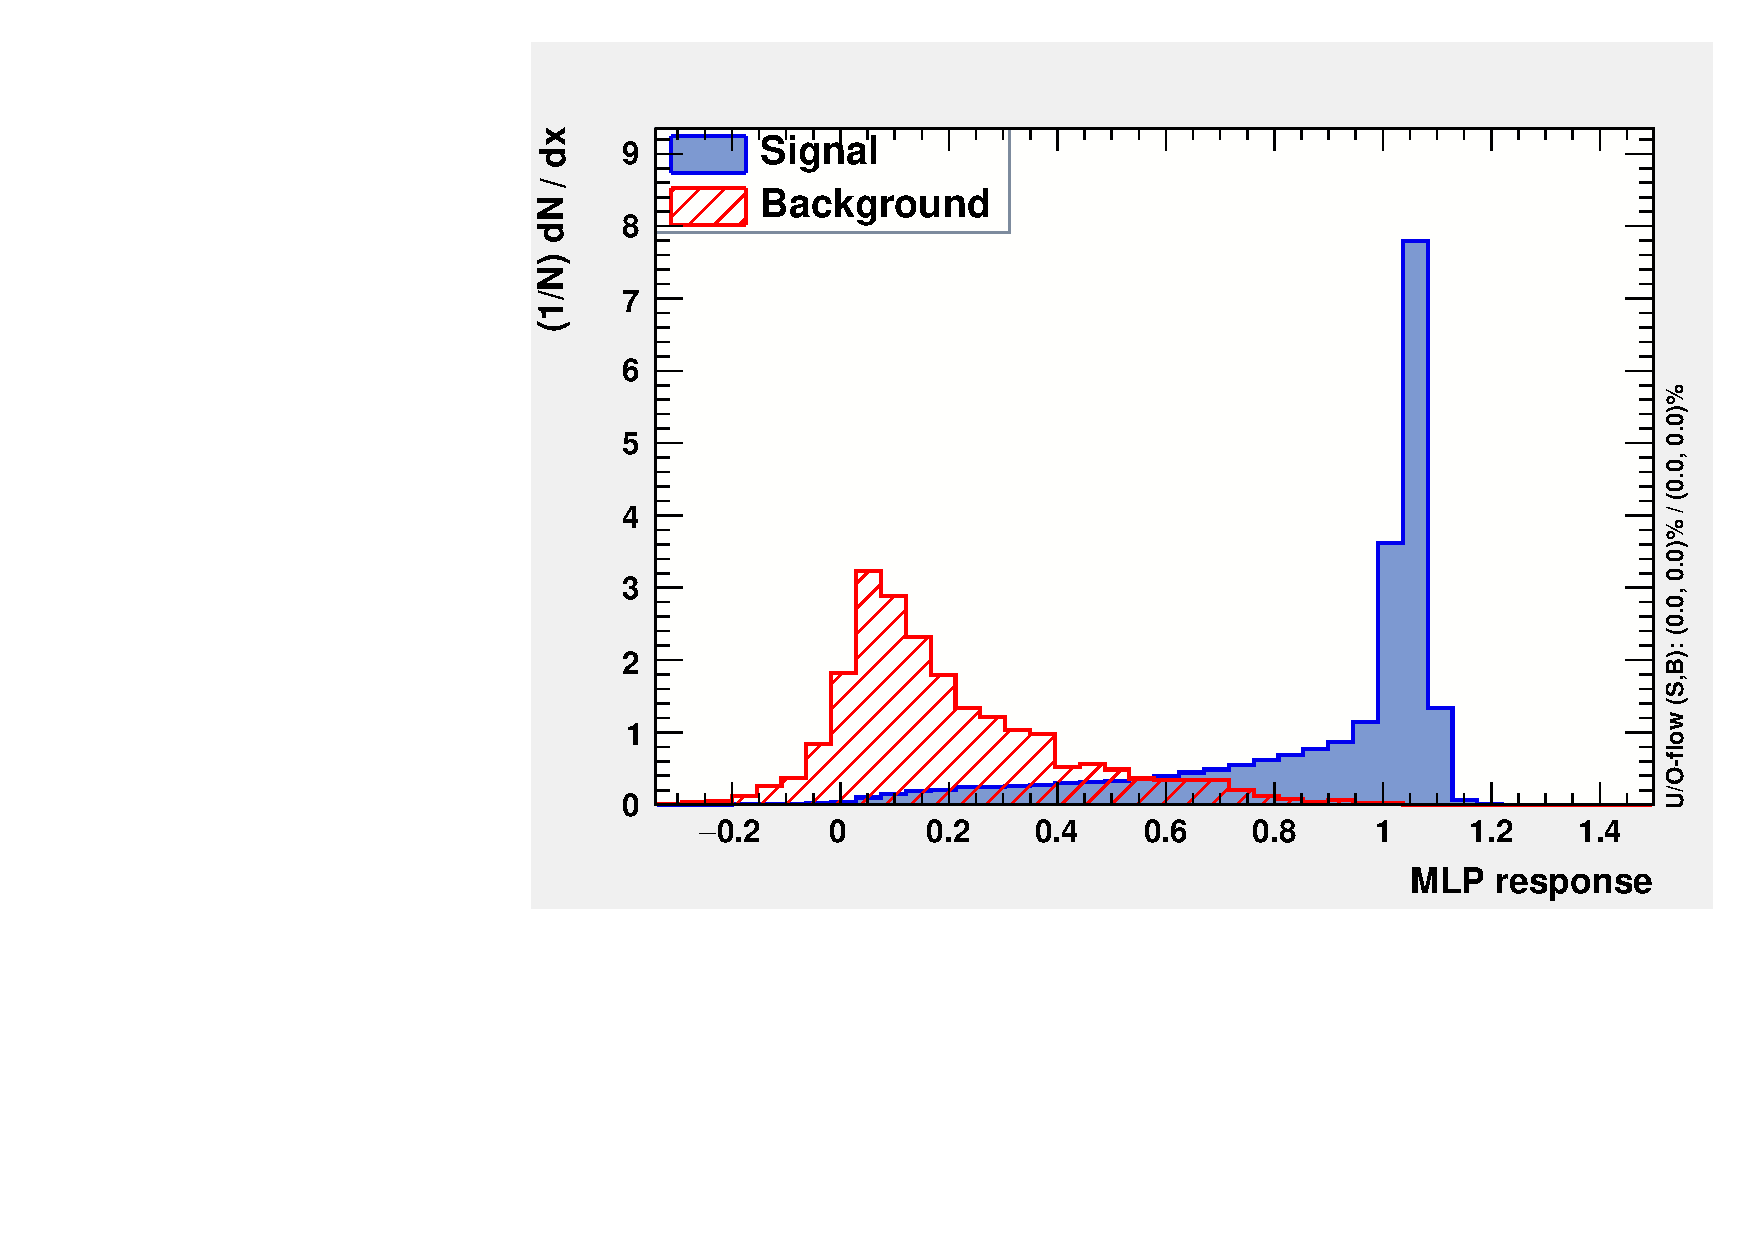
\includegraphics[width=8cm]{output_allE_MLP.pdf}
		\end{minipage}
	}
	\caption{TMVA outputs for signal/background separations by different methods, for the $4<E<15$ MeV testing dataset.\label{output_separation_allE}}
\end{figure}

As one of the essential TMVA outputs, the background rejection versus signal efficiency curve is denoted as a receiver operating characteristic (ROC) curve, which is usually used to test the performance of a machine learning classifier. The integral of the ROC curve, named ``area under the curve'' (AUC), is often used to summarize the quality of an ROC curve \cite{murphy2012machine}.  Fig.~\ref{fig:energyVsROC} shows the ROC curves for three different methods and for the testing datasets with different energy regions.

\begin{figure}[htbp]
	\centering
	\subfigure[$4<E_{fit}<15$~MeV.]{
		\begin{minipage}[t]{0.5\textwidth}
			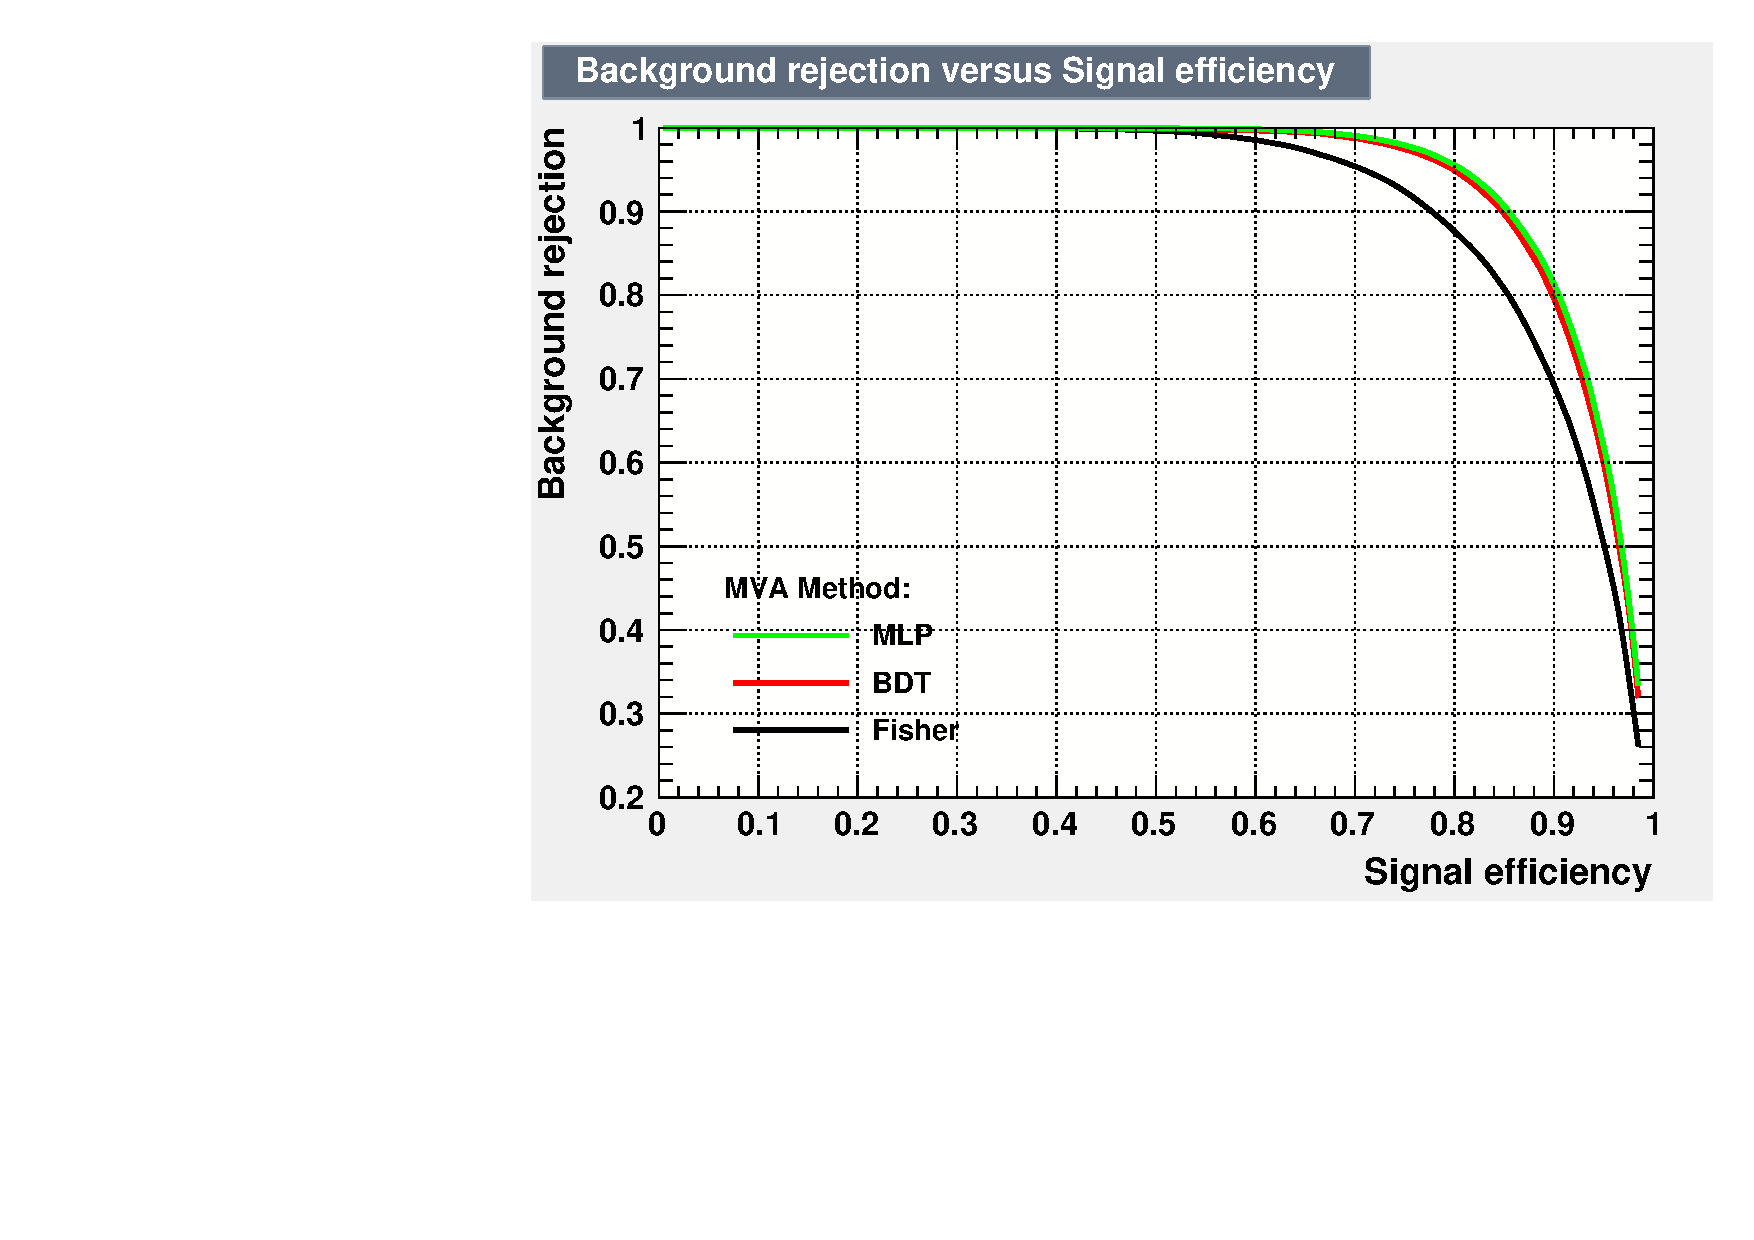
\includegraphics[width=8cm]{ROC_E4to15.pdf}
		\end{minipage}
	}
	\subfigure[$5<E_{fit}<15$ MeV (energy above 5 MeV).]{
		\begin{minipage}[b]{0.4\textwidth}
			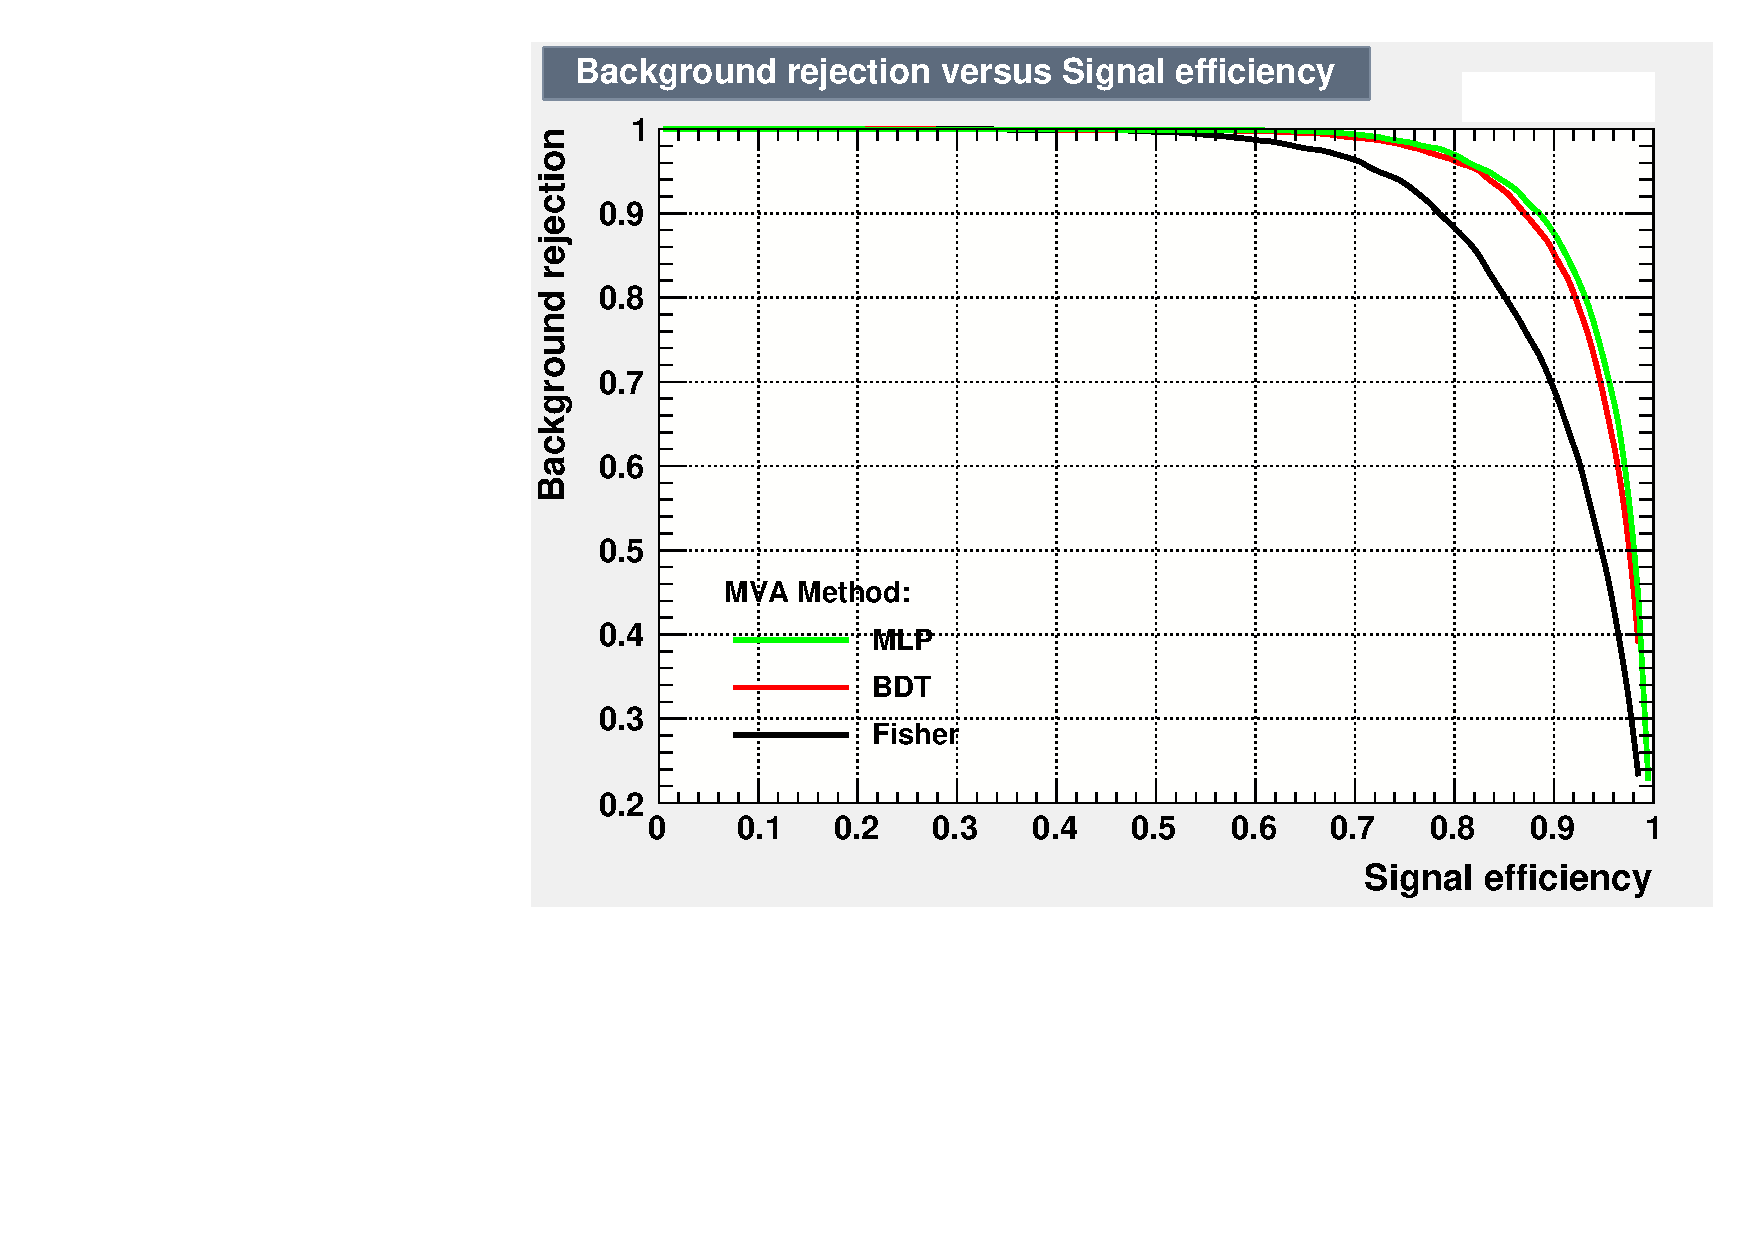
\includegraphics[width=8cm]{ROC_E5to15.pdf}
		\end{minipage}
	}
	\subfigure[$4<E_{fit}<5$~MeV.]{
		\begin{minipage}[b]{0.4\textwidth}
			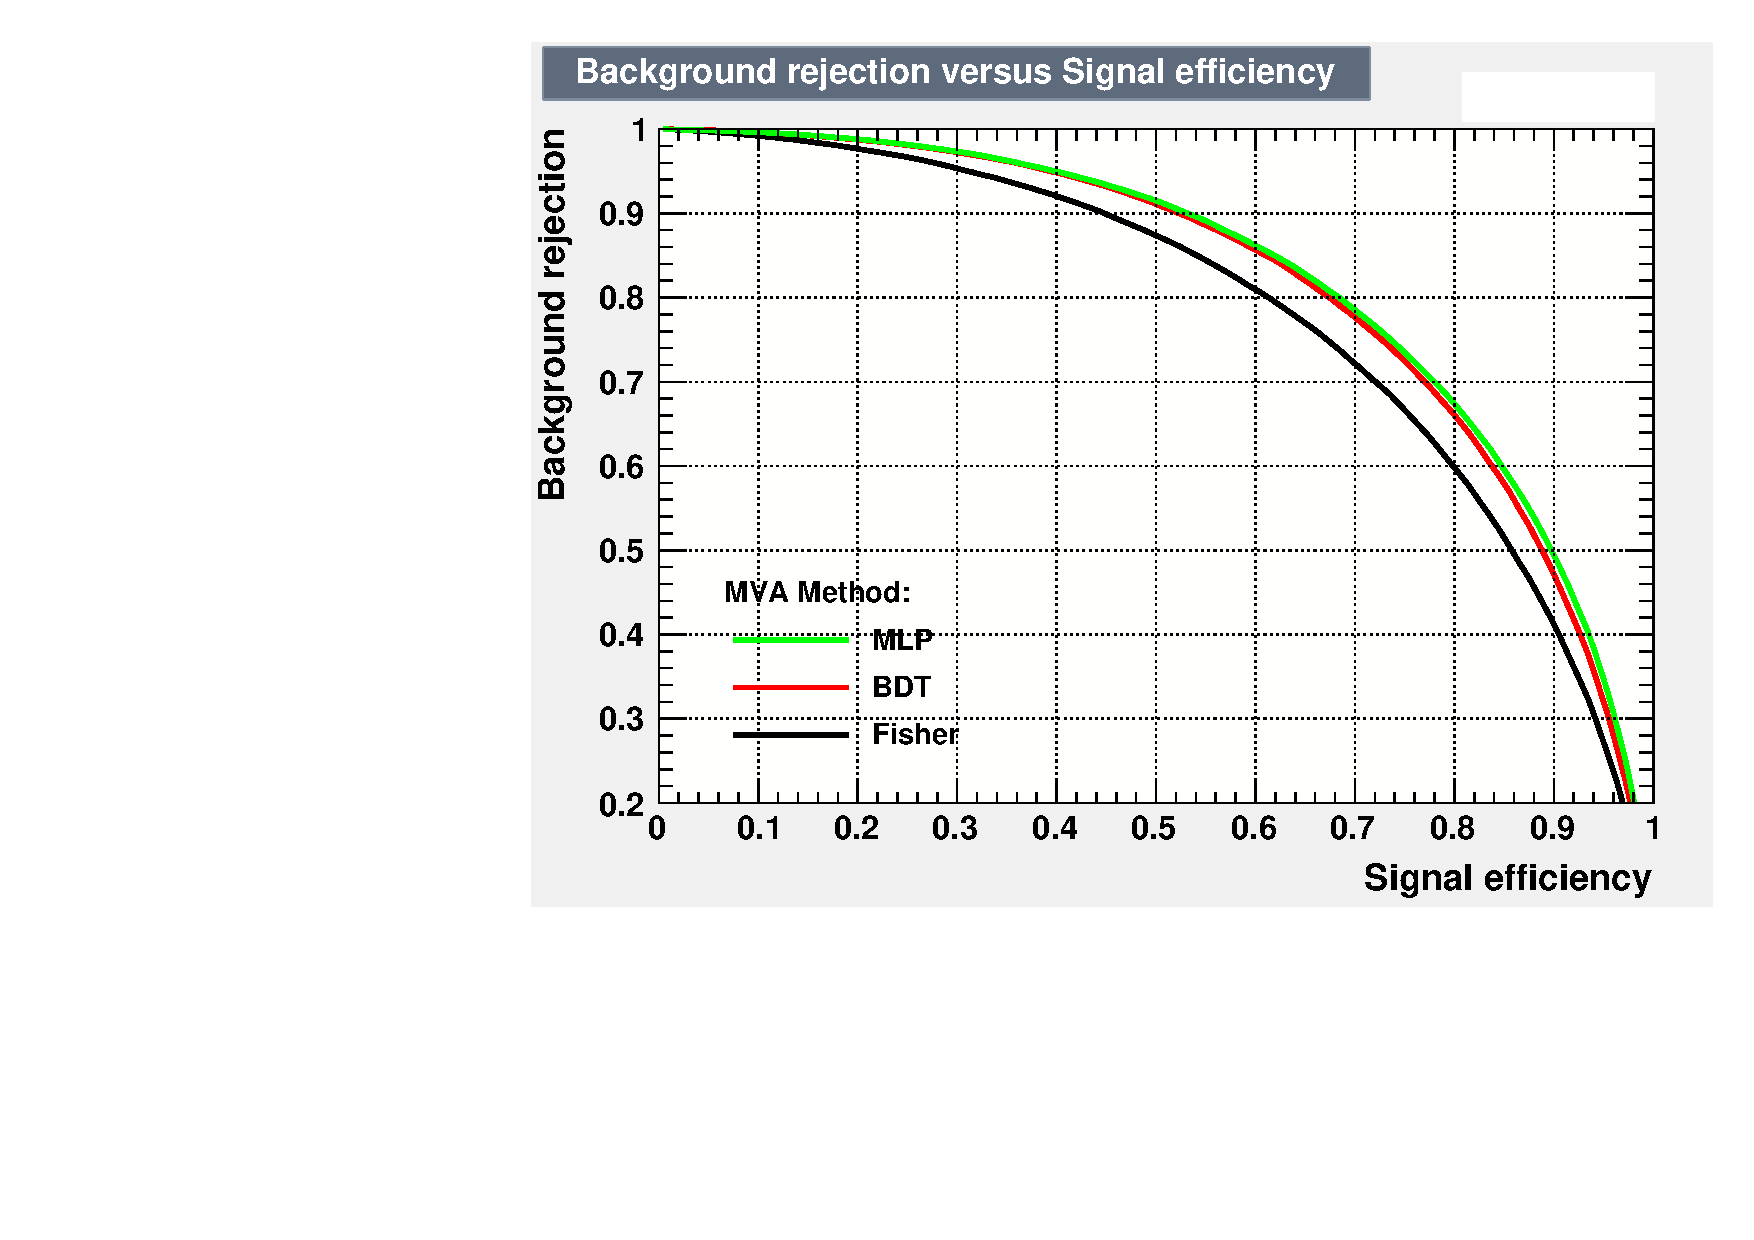
\includegraphics[width=8cm]{ROC_E4to5.pdf}
		\end{minipage}
	}
	\caption[TMVA outputs for signal/background separations by different methods]{TMVA outputs for signal/background separations by different methods, for the $4<E<15$ MeV, $5<E<15$ MeV, and $4<E<5$ MeV testing dataset.\label{fig:energyVsROC}}
\end{figure}

Typical CPU times ($t_{CPU}$) to train each algorithm for chosen energy regions are listed in Table.~\ref{tab:tmvaMethod_allE}.
\begin{table}[ht]
	\centering
	\caption{Testing results from different TMVA methods.}
	\label{tab:tmvaMethod_allE}
	\begin{tabular*}{100mm}{c@{\extracolsep{\fill}}ccc}
		\toprule
		Method & AUC & $t_{CPU}$ (second/$10^6$ events) \\
		\midrule
		$4<E_{fit}<15$~MeV \\
		Fisher/LD & 0.915 & 0.81\\
		BDT &  0.940 & 249.53 \\
		MLP & 0.944 & 1370.02\\
		\hline
		$5<E_{fit}<15$ MeV\\
		Fisher/LD & 0.915& 0.93\\
		BDT & 0.950 & 269.71\\
		MLP &  0.958 & 1450.90\\
		\hline
		$4<E_{fit}<5$ MeV \\
		Fisher/LD & 0.782 & 0.84\\
		BDT & 0.816 & 280.1\\
		MLP & 0.823 &1337.9\\
		\bottomrule
	\end{tabular*}
\end{table}

The testing results in Table.~\ref{tab:tmvaMethod_allE} show that the Fisher/LD output gives the worst AUC. The BDT and MLP outputs are close to each other while the MLP gives the largest AUC values. However, the MLP was the expensive method in terms of CPU usage. All three methods are less successful in  separating signal from backgrounds in the lower energy region.

The distributions of $\cos\theta_\mathrm{sun}$ were used to show the performance of the solar $\nu_e$ event selection and background event discrimination. Here I applied the BDT and the MLP method on the test sub-dataset. For the real dataset from run-200004 to 207718, the trained weights and variables from the BDT and the MLP methods were applied event by event and the discriminator responses, $D_{BDT}$ and $D_{MLP}$ were calculated respectively. Cuts of $D_{BDT}>0.0$ and $D_{MLP}>0.5$ were applied to extract the solar $\nu_e$ signals from backgrounds. 
%The distributions of $\cos\theta_\mathrm{sun}$ were shown in Fig. as the results.
%4<E<15 MeV
%%BDT signal efficiency     = 0.944954
%% MLP signal efficiency        = 0.926606

%MLP signal efficiency        = 0.842493
%MLP background efficiency    = 0.0840084
%5<E<15 MeV
%BDT signal efficiency     = 0.868345w
%BDT background efficiency = 0.103896
%MLP signal efficiency        = 0.887622
%MLP background efficiency    = 0.104416

%%% BDT signal efficiency     = 0.733945
%% MLP signal efficiency        = 0.779817
%
%4<E<5 MeV
%BDT signal efficiency     = 0.72266
%BDT background efficiency = 0.245453
%MLP signal efficiency        = 0.723576
%MLP background efficiency    = 0.235984

%\begin{figure}[!htb]
%	\centering
%	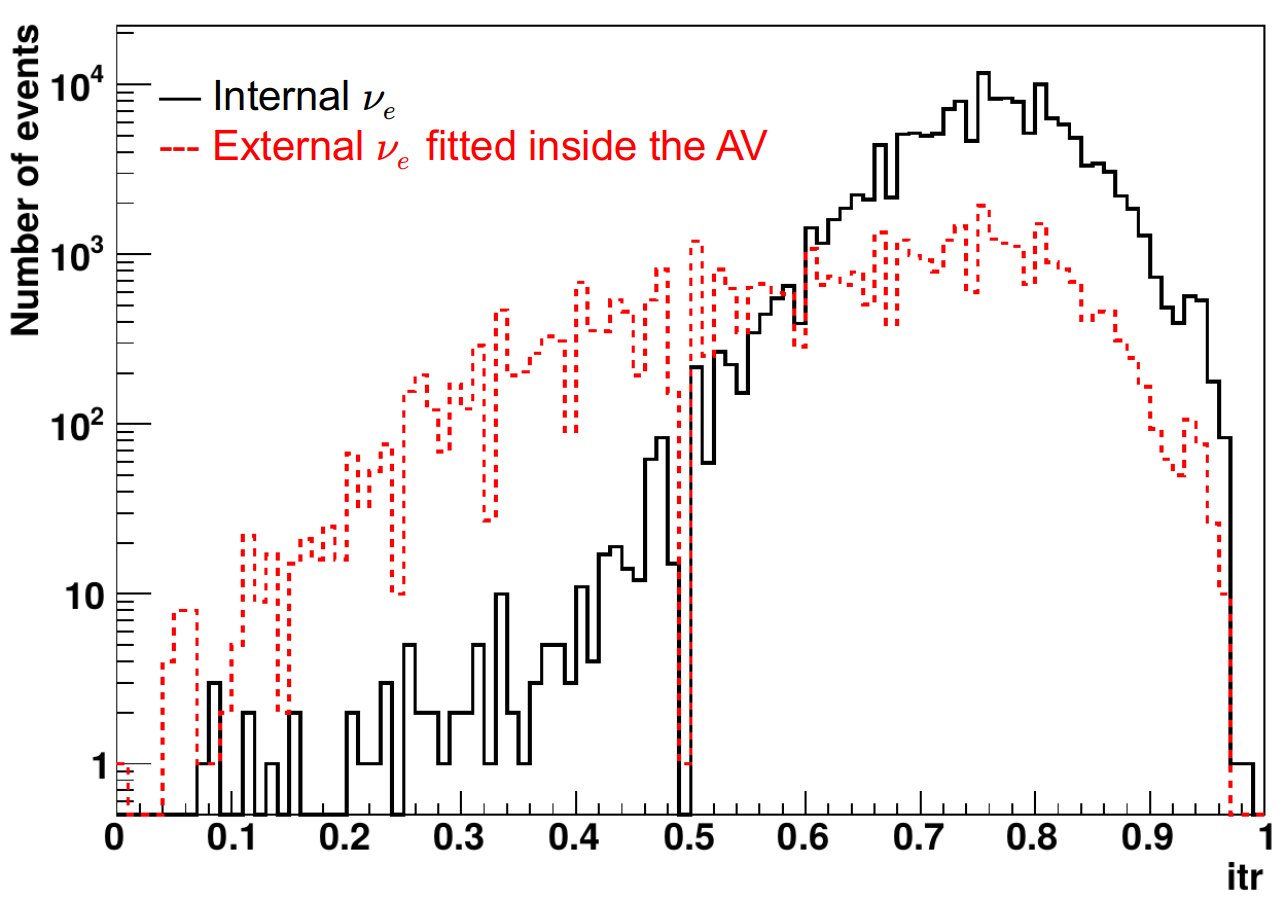
\includegraphics[width=8cm]{ITR_MPW_solarNuVsExSolar.png}
%	\caption{Comparison between solar $\nu_e$ and external solar $\nu_e$; MPW results.}
%	\label{itrCmp}
%\end{figure}
\subsection{TMVA Outputs}

The trained weights were applied to both the simulations and the actual data from the 92.54 live-day half-dataset.  Fig.~\ref{fig:cosThetaToSun_4to15_output} shows the results provided by the BDT and MLP selections for the $4<E<15$ MeV region. The BDT selection classifies about 80.8\% of the total data as background events while the MLP classifies about 76.17\% as background. Rather flat distributions for  $\cos\theta_\mathrm{sun}$ are apparent the plots. Since background events are predominant in the $4<E<5$ MeV region, the analyses to follow will focus only on the $5<E<15$ MeV region.

\begin{figure}[!htb]
	\centering
	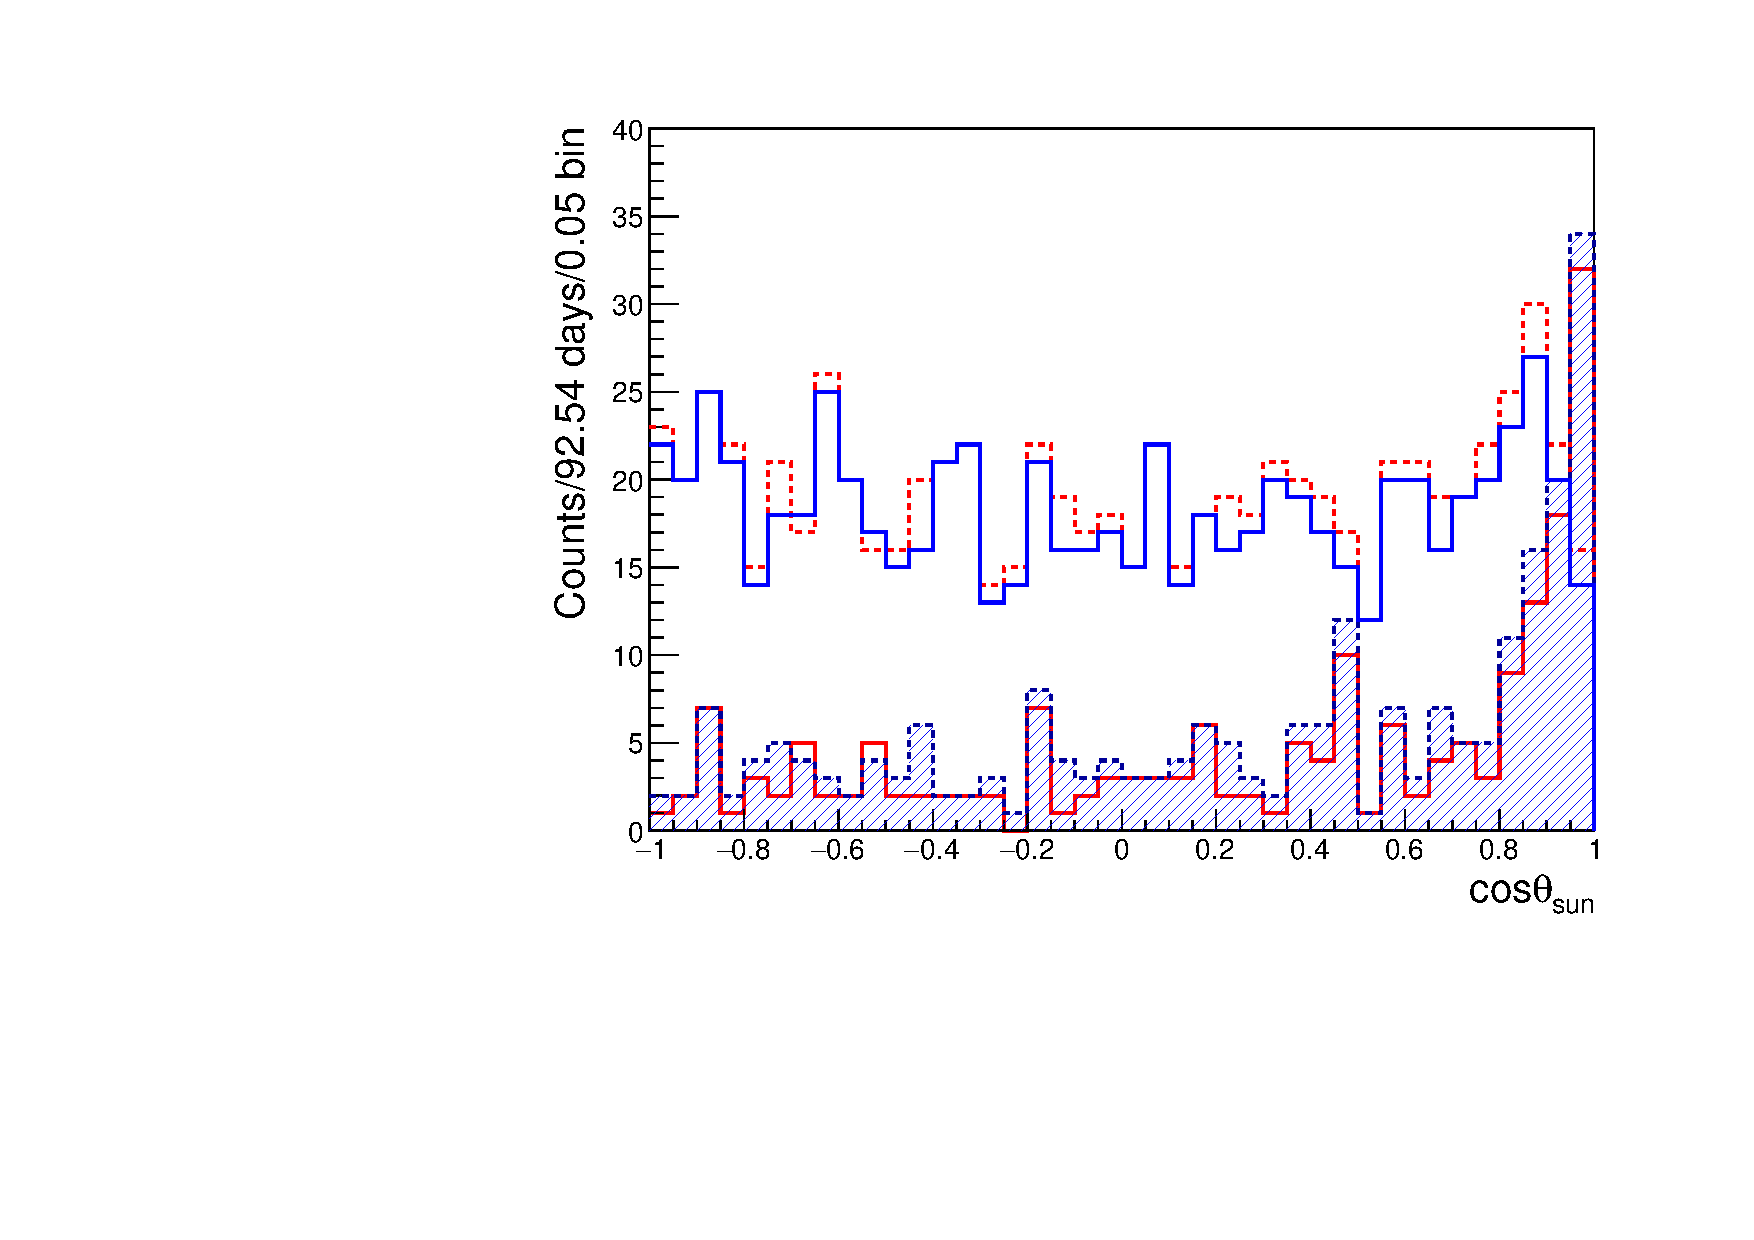
\includegraphics[width=10cm]{cosThetaToSun_4to15_output.pdf}
	\caption[BDT and MLP outputs for the $\cos\theta_\mathrm{sun}$, with $4<E_{fit}<15$ MeV.]{BDT and MLP outputs for $\cos\theta_\mathrm{sun}$, in the $4<E_{fit}<15$ MeV energy range. The solid red line shows the BDT-selected candidate solar $\nu_e$ events, while the blue shaded histogram shows the MLP-selected ones. The dotted red line is for BDT-selected backgrounds, while the solid blue line is for the MLP-selected backgrounds.\label{fig:cosThetaToSun_4to15_output}}
\end{figure}

To test the outputs, the same fake datasets mentioned in Sect.~\ref{sect:ensemble} were used. Fig.~\ref{fig:BDToutputs} shows the BDT output distributions of the $\cos\theta_\mathrm{sun}$ for one random fake dataset, for event energy range $5<E_{fit}<15$ MeV. The output after the default cuts is also shown here as a comparison. For this fake dataset, the true number of signal and background events are: $N^{true}_{sig}=68$ and $N^{true}_{bkg}=46$, while the BDT outputs are $N^{BDT}_{sig}=61$ and $N^{BDT}_{bkg}=53$. This indicates an underestimate of the signal ($N^{BDT}_{sig}=0.90 N^{true}_{sig}$) and an overestimate of the background ($N^{BDT}_{sig}=1.15 N^{true}_{sig}$). 

\begin{figure}[!htb]
	\centering
	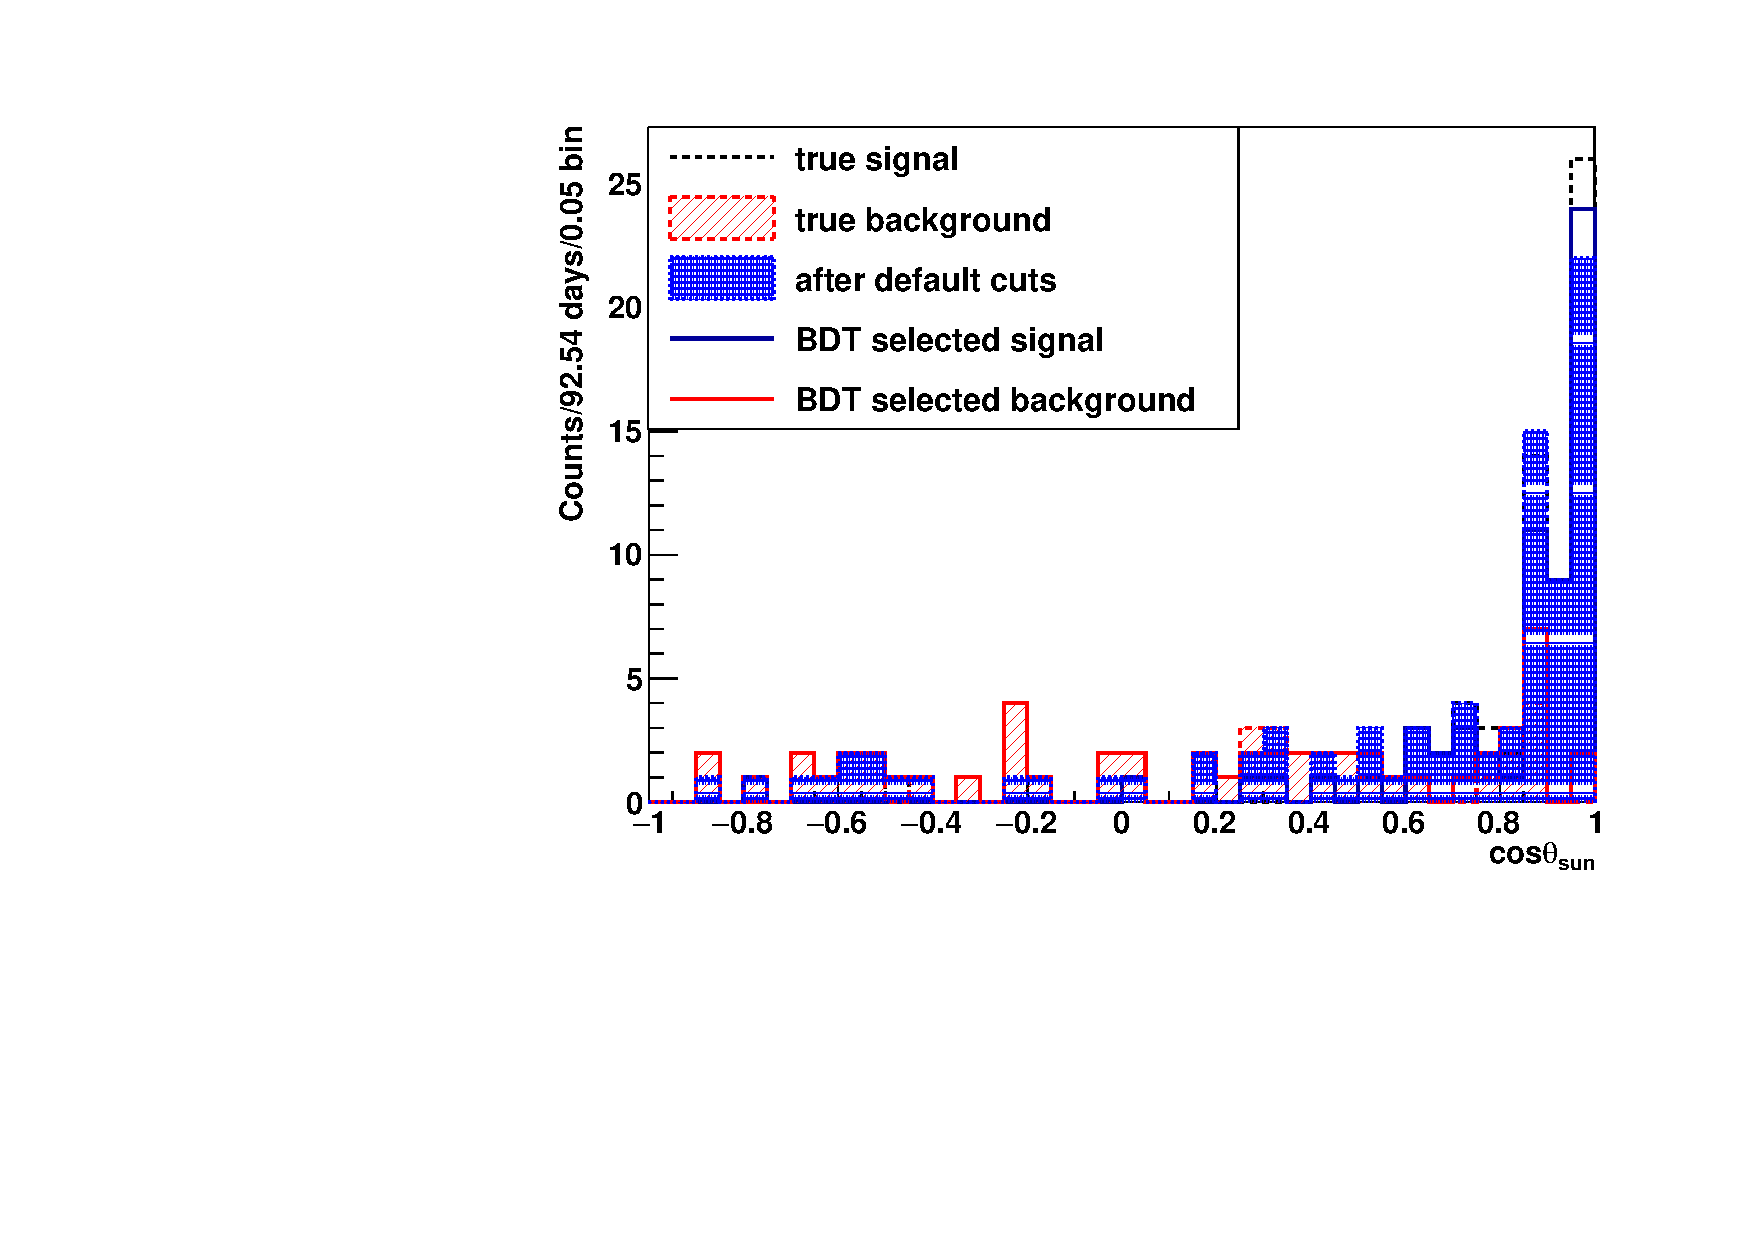
\includegraphics[width=10cm]{tmvaHalfFakeData_output.pdf}
	\caption[BDT outputs from one random fake dataset, with $5<E_{fit}<15$ MeV.]{BDT outputs from one random fake dataset, with $5<E_{fit}<15$ MeV. The solid blue line and the solid red line are for the BDT output of the signal and background events, respectively; the dashed black line and the shaded red histogram are for the true signal and background events, respectively. Finally, the results after the default cuts are shown in the blue shaded area.\label{fig:BDToutputs}}
\end{figure}

As shown in Fig.~\ref{fig:TMVAfractions}, applying the TMVA BDT selection to each of 5000 fake dataset, the ratios of the BDT-selected event count to the true event count are $(91.26\pm 4.77)\%$ for signal events, and $(117.1\pm 10.46)\%$ for background events (using the histogram mean and root mean square). 

\begin{figure}[!htb]
	\centering
	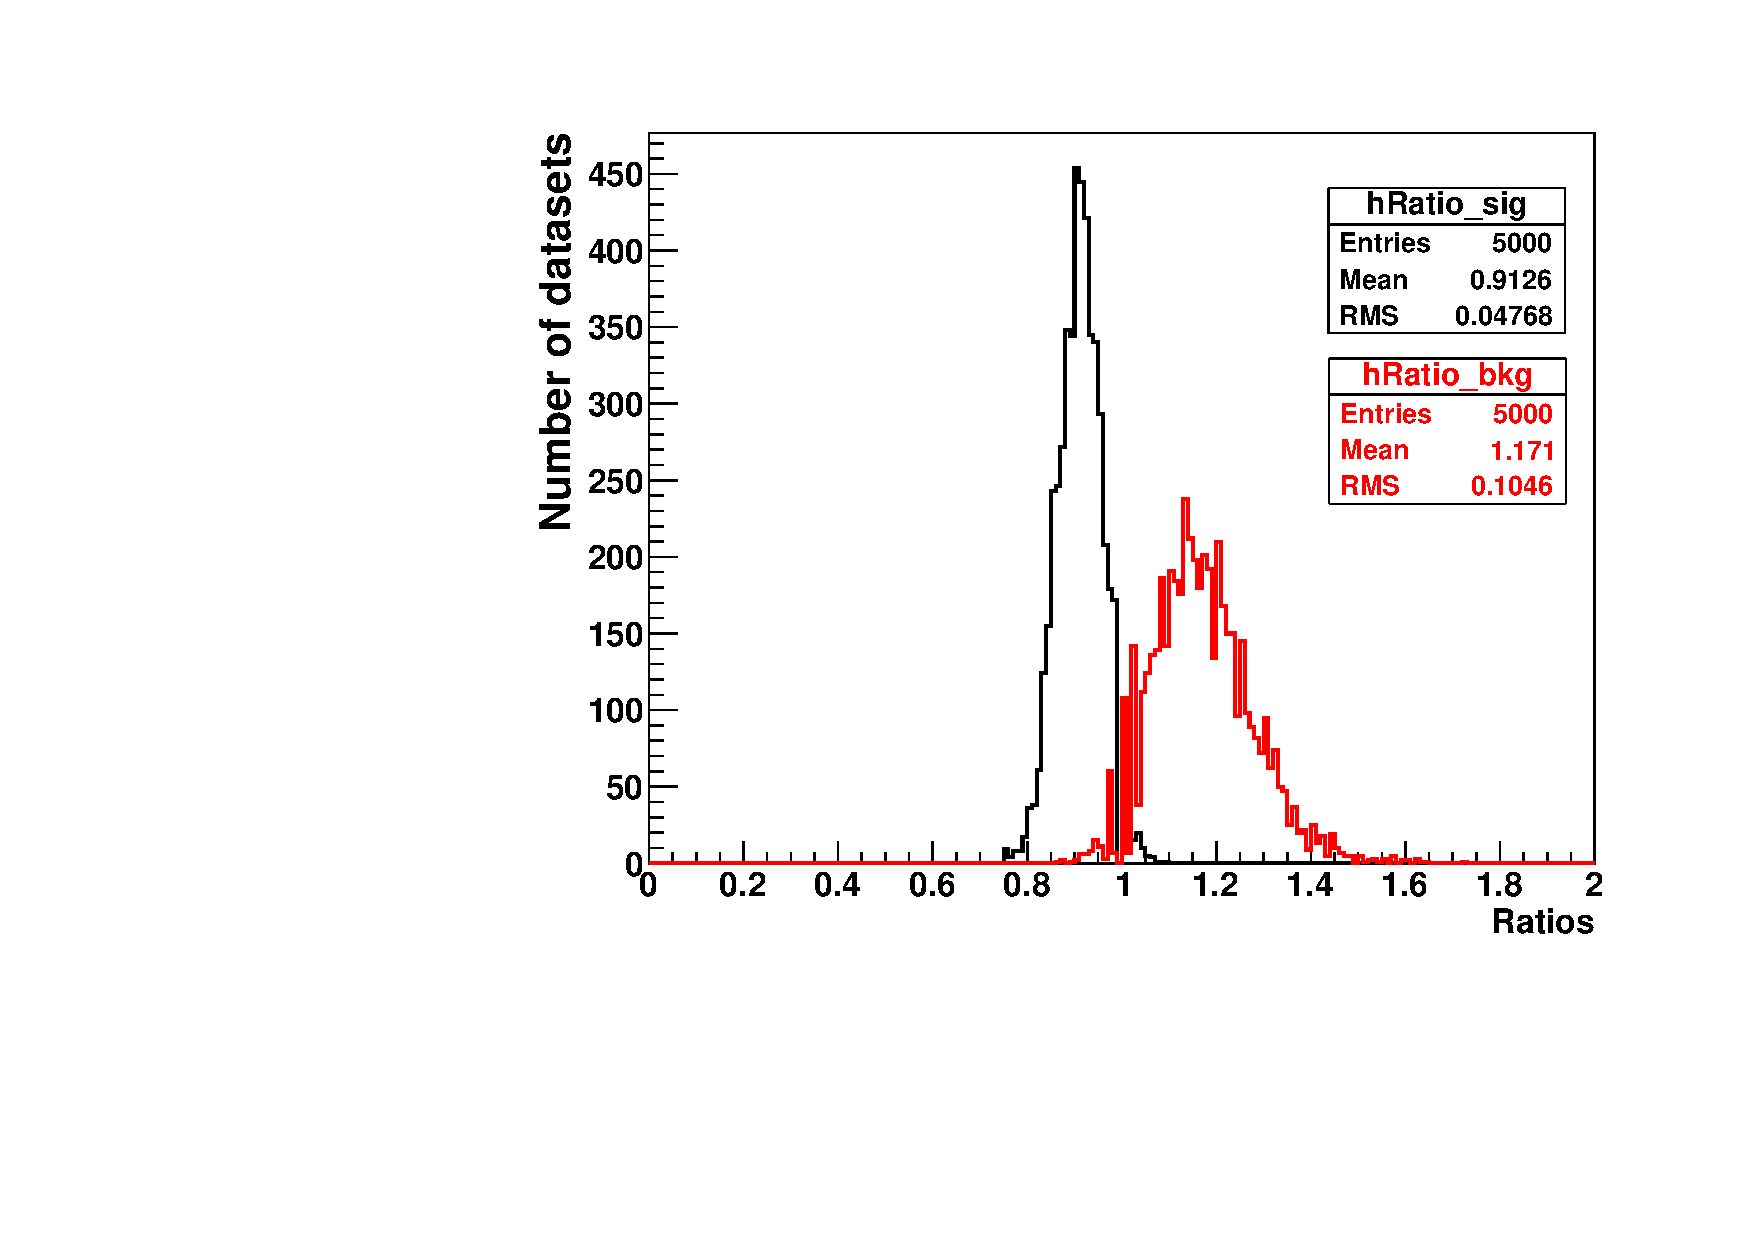
\includegraphics[width=10cm]{TMVAratios_fakedataset.pdf}
	\caption[Event count fractions from BDT outputs on 5000 fake datasets, with $5<E_{fit}<15$ MeV.]{Event count ratios from BDT outputs on 5000 fake datasets, with $5<E_{fit}<15$ MeV. The black histogram is the distribution of the signal fraction, and the red histogram is the distribution of the background fraction.\label{fig:TMVAfractions}}
\end{figure}

In this case, although the number of signal events is underestimated, the TMVA methods do succeed to remove most of the background events. Also, for the Poisson fit, the TMVA methods were also applied to the MC simulations used as PDFs, these effects can be neutralized in fitting the events. Sect.~\ref{sect:fitTheWhole} will show the fit of the TMVA outputs for the whole dataset. 

\subsection{Discussions of TMVA Results}

The TMVA methods optimize the cuts on more variables (FoMs and $klDiv$) and make more stringent cuts to reduce the background events compared to the beforehand cuts. A more stringent radial cut (or tighter FV) can be applied on the low energy region $4<E_{fit}<5$~MeV to eliminate further background events, which dominate in that region. However, tighter cuts can also eliminate the signal events.

Other packages developed for high energy particle physics, such as \texttt{StatPatternRecognition} (SPR) \cite{sprWebsite}, can also be considered as an alternative tool or as a reference for results comparisons. 

\subsection{Fitting Whole Low Background Dataset}\label{sect:fitTheWhole}
To combine the analyses in the previous two sections, the TMVA selection methods were applied to the actual data of the 190.33 live-day whole dataset and then a maximum likelihood fit was applied on the selected data. 

For the whole dataset, the TMAV methods were applied to the whole MC datasets of the solar $\nu_e$ simulations as well as the background simulations\footnote{The simulations of solar $\nu_{\mu}$ were also trained with the background simulations separately to calculate the detected $\nu_\mu$ from the oscillated solar neutrino flux mentioned in next section}. Similarly, the training subset used 70.25\% of the whole dataset (run-200004 to 205296), while the testing subset used the rest 29.75\% (run-205297 to 207718). The trained BDT and MLP weights were applied to the whole dataset.

In the region of $5<E_{fit}<15$~MeV, the outputs from the BDT and MLP were fitted to obtain $N_{sig}$ and $N_{bkg}$. Fig.~\ref{fig:wholeDataset_poissonFit} show their results respectively. For comparison, the results from applying the default cuts are shown below. The fit results are summarized in Table.~\ref{table:wholedata_output}. 
%{John: try not to use of "also" over and over as a way to give continuity}

\begin{figure}[!htb]
	\centering
	\subfigure[BDT.]{ 
		\begin{minipage}[t]{0.5\textwidth}
			\centering
				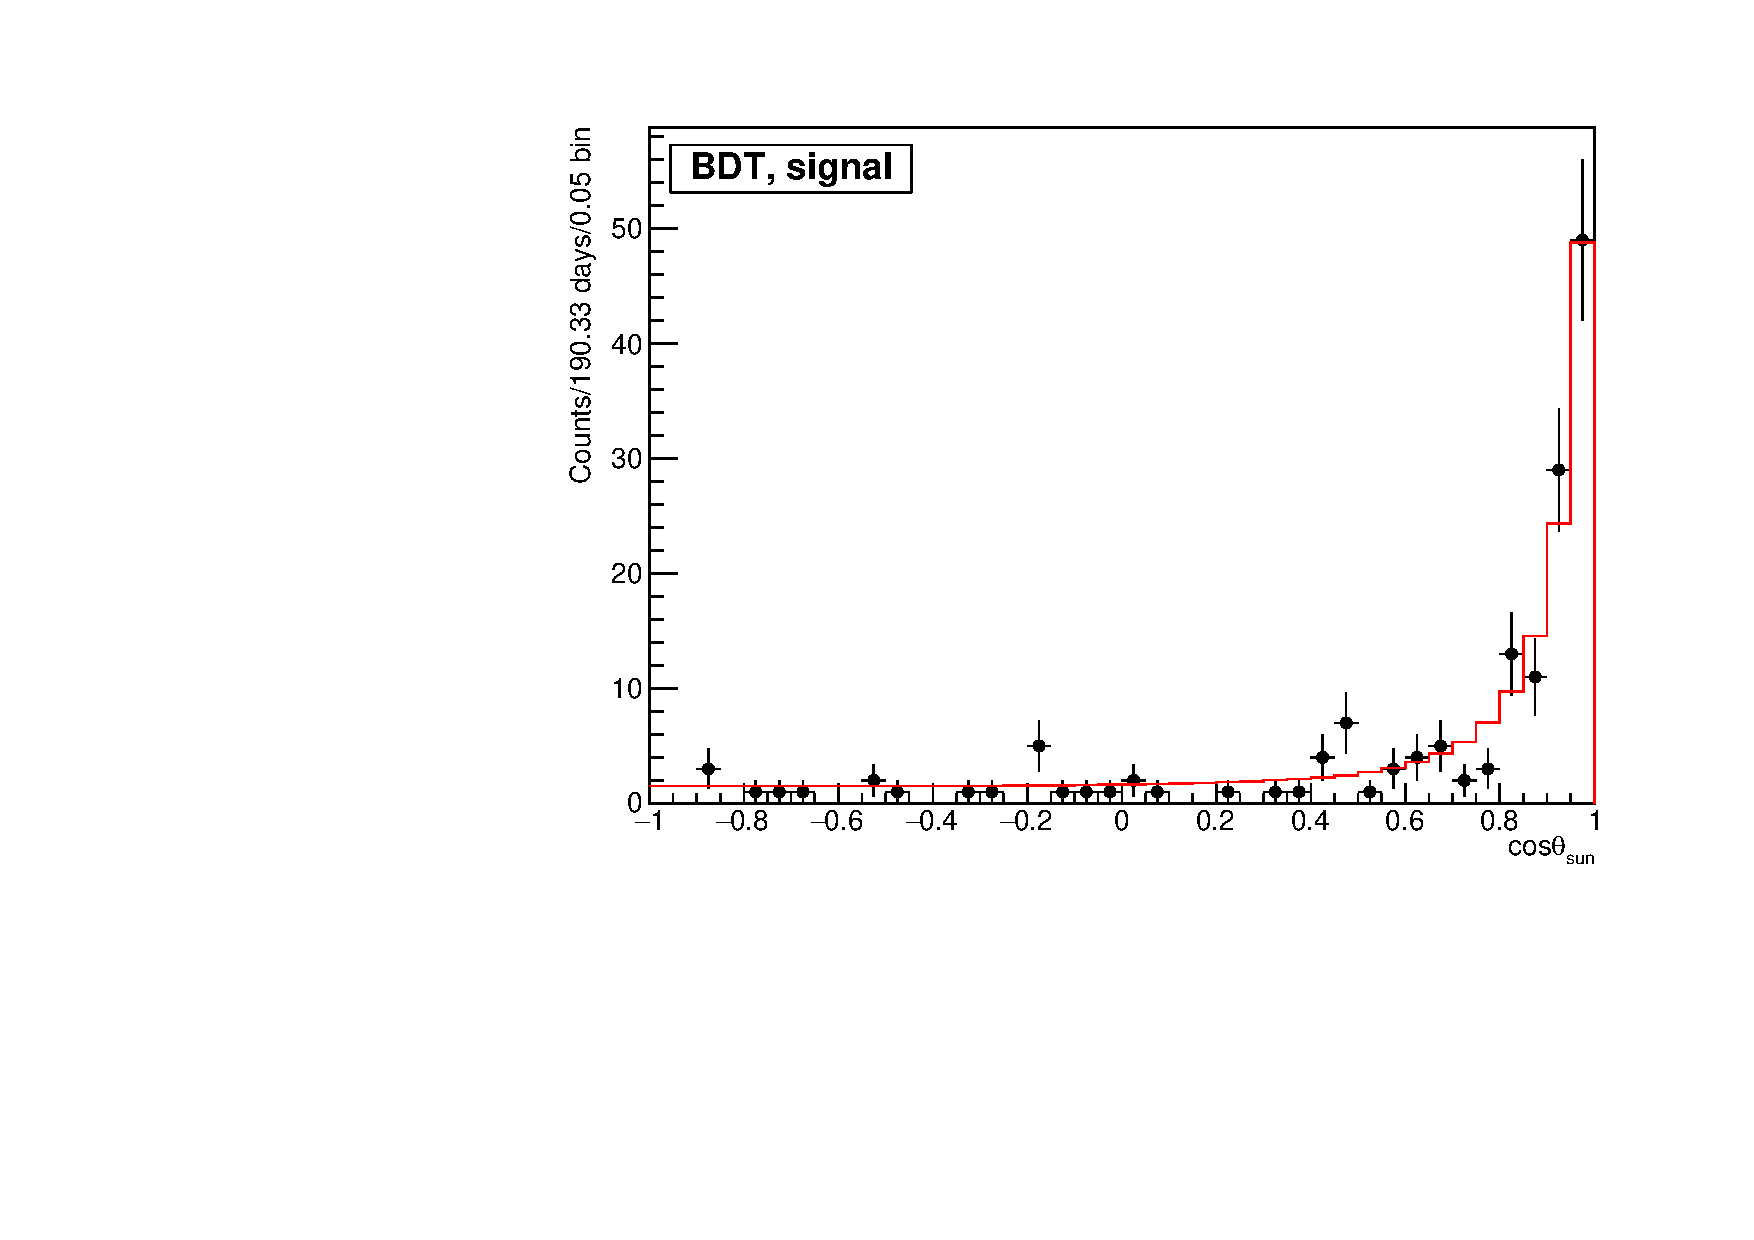
\includegraphics[width=8cm]{wholedataFit_bdt.pdf}
		\end{minipage}
	}
	\subfigure[MLP.]{ 
		\begin{minipage}[t]{0.4\textwidth}
			\centering
			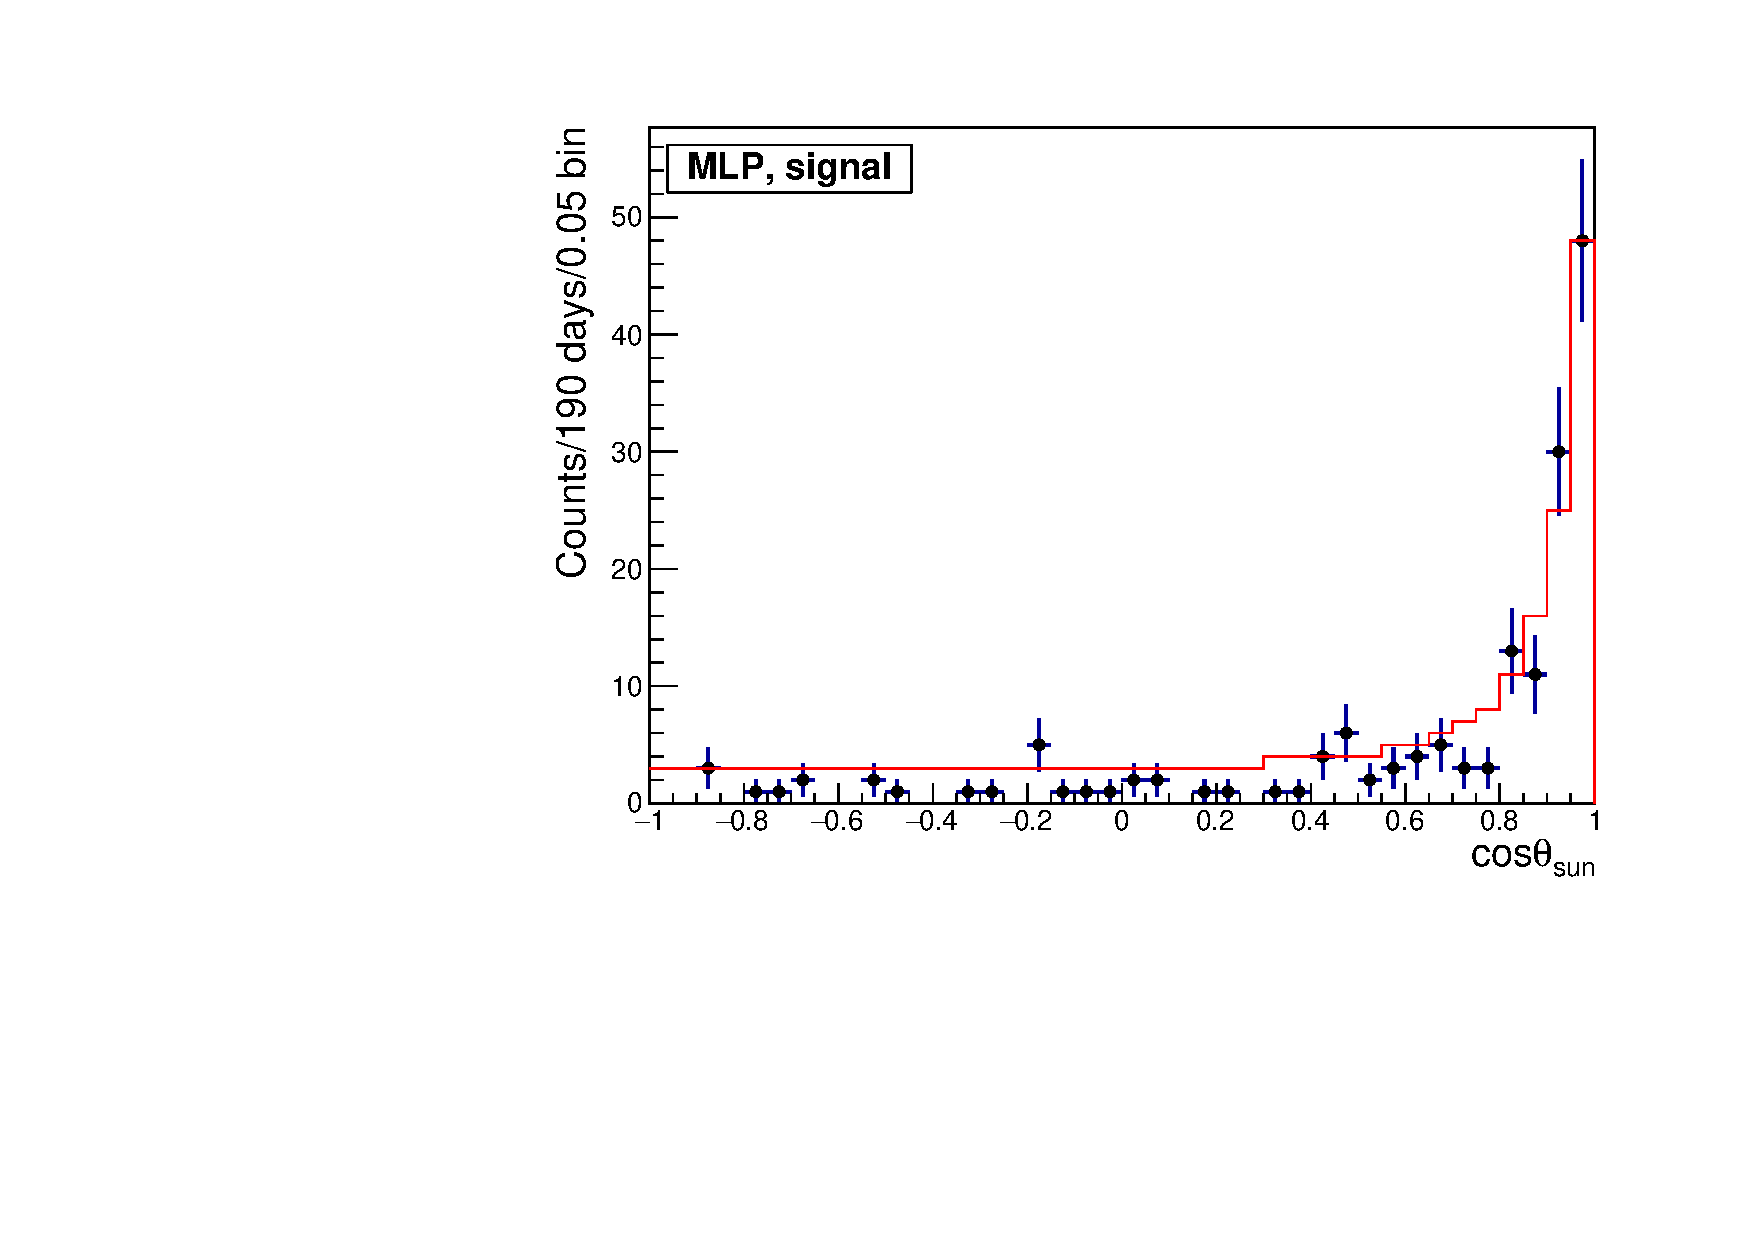
\includegraphics[width=8cm]{wholedataFit_mlp.pdf}
		\end{minipage}
	}
	\subfigure[Default cuts.]{ 
		\begin{minipage}[b]{0.4\textwidth}
			\centering
			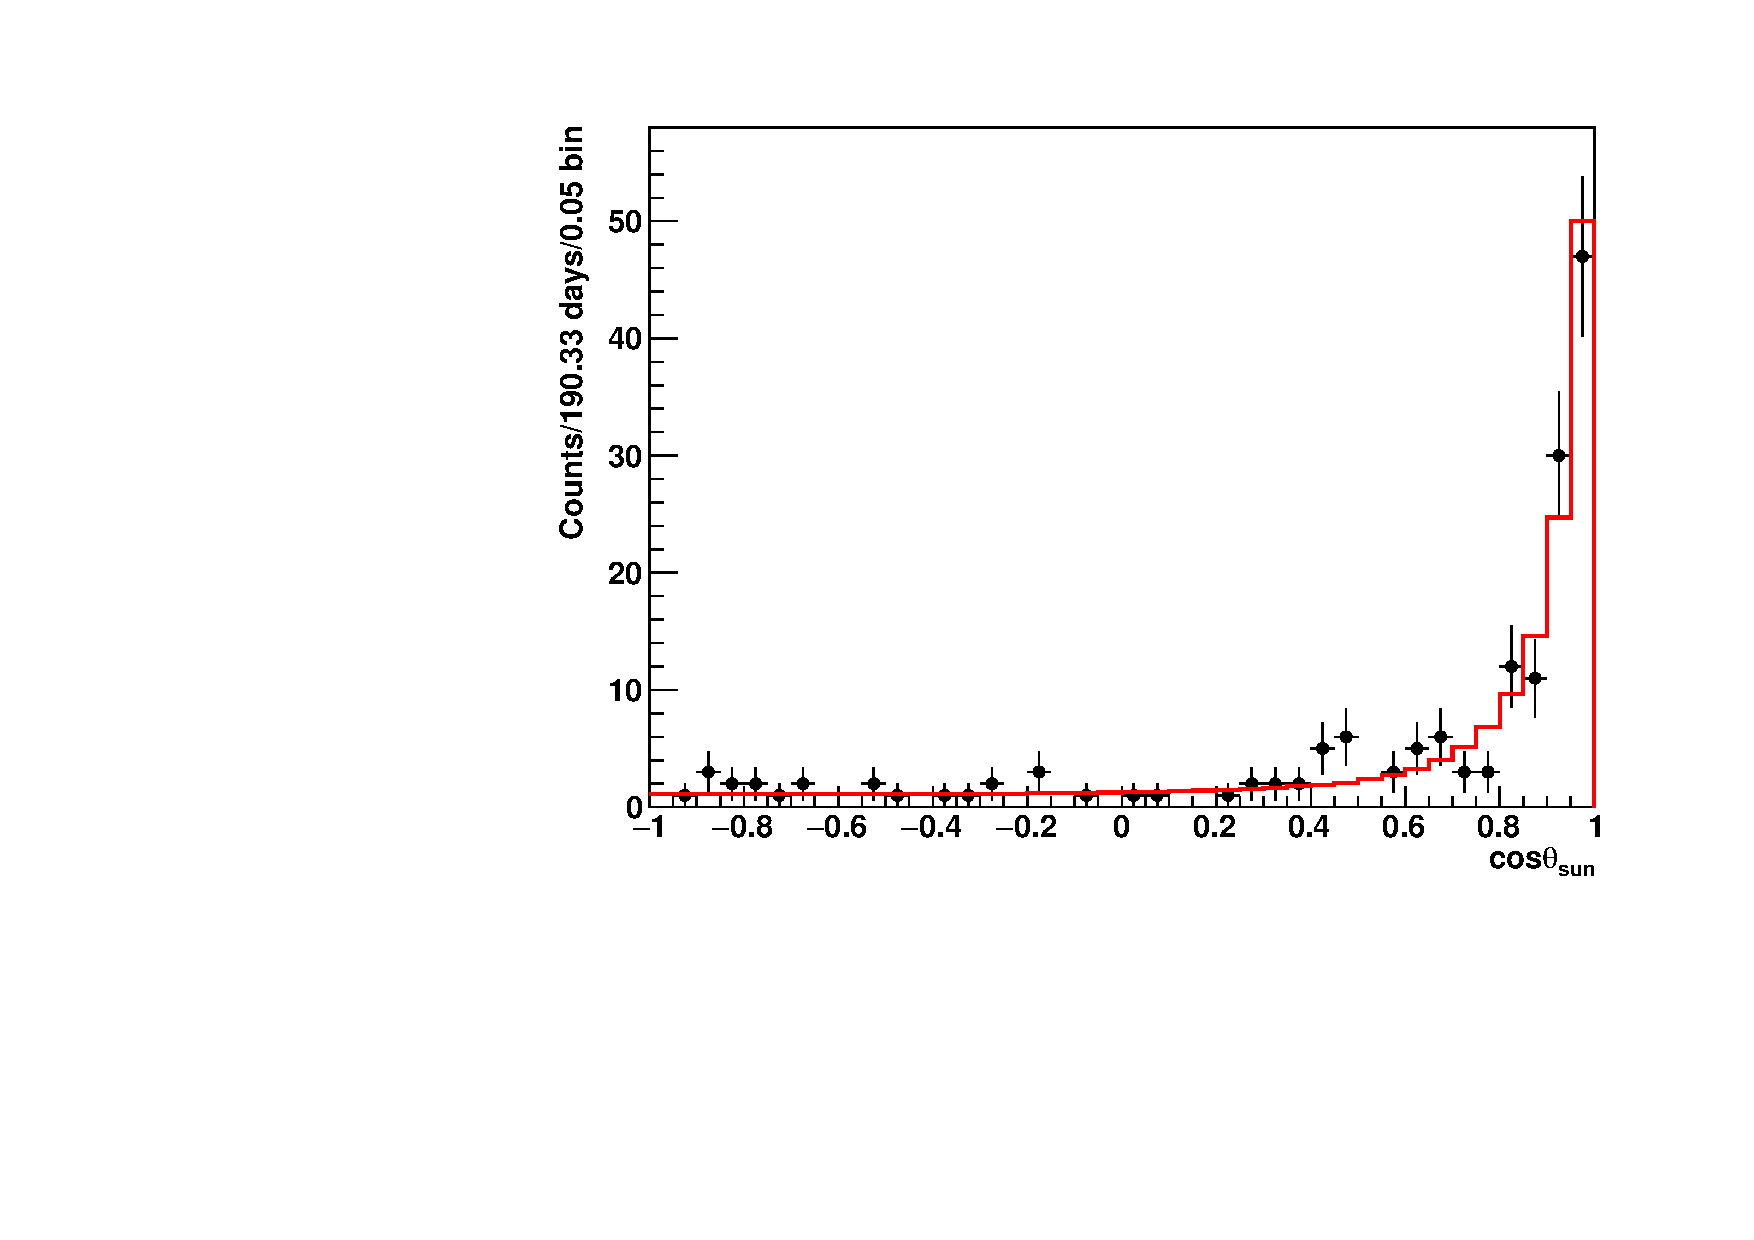
\includegraphics[width=8cm]{wholeDataset_defaultCuts.pdf}
		\end{minipage}
	}
	\caption[Poisson fit results for the $5<E_{fit}<15$~MeV.]{Poisson fit results for the $5<E_{fit}<15$~MeV range, from the outputs of BDT (a), MLP (b), and default cuts (c).\label{fig:wholeDataset_poissonFit}}
\end{figure} 

\begin{table}[ht]
	\centering
	\caption{Fit results for the whole dataset ($5<E<15$~MeV).}
	\label{table:wholedata_output}
	\begin{tabular*}{150mm}{c@{\extracolsep{\fill}}cccccc}
		\toprule
		Methods & $N_{sig}$ & $N_{bkg}$ & $R_{sig}$ & $R_{bkg}$ & $p-value$ \\
		\hline
		BDT &$119.57\pm11.88$ & $38.42\pm7.75$ & $0.90\pm0.09$ & $0.29\pm0.06$ & 0.14\\
		MLP &$118.77\pm11.84$ & $40.22\pm7.85$ & $0.90\pm0.09$  & $0.30\pm 0.06$  & 0.18\\
		Default Cuts & $119.33\pm 11.96$ & $42.67\pm 8.15$ &  $0.90\pm 0.09$ & $0.32\pm0.06$ & 0.19\\
		\bottomrule
	\end{tabular*}
\end{table}

Results from the three methodologies are consistent with each other. The estimated background rate in the [5,15] MeV energy region is about $\frac{1}{3}$ of the signal rate, which indicates that a low background measurement is achieved for the solar neutrino analysis with the energy down to 5 MeV. For the sake of simplicity, since the output from the BDT selection gives a better $p-\mathrm{value}$, the analyses to follow will use only the BDT selector. 

\subsection{Evaluating $^8$B Solar Neutrino Flux}\label{sect:evaluateFlux}

A program called \texttt{PSelmaa} (Physics interpretation Sun-Earth Large Mixing Angle Adiabatic
Approximation) was implemented in \texttt{RAT} \cite{fady_pselmaa}. The software uses the BS05(OP) SSM model. It assumes the normal mass hierarchy, and it applies the MSW effects due to the Sun (see Chapter 2) but neglects the MSW effects due to the Earth (i.e., the regeneration of coherence in the Earth). Fig.~\ref{fig:pselmaa_curves} shows the survival probability curve as a function of energy (in 0.1 MeV intervals) taken from the \texttt{PSelmaa}. (As SNO+ can not discriminate $\nu_\mu$ and $\nu_\tau$, only the $\nu_\mu$ MC is included in $P_{e\alpha}$.)

\begin{figure}[!htb]
	\centering
	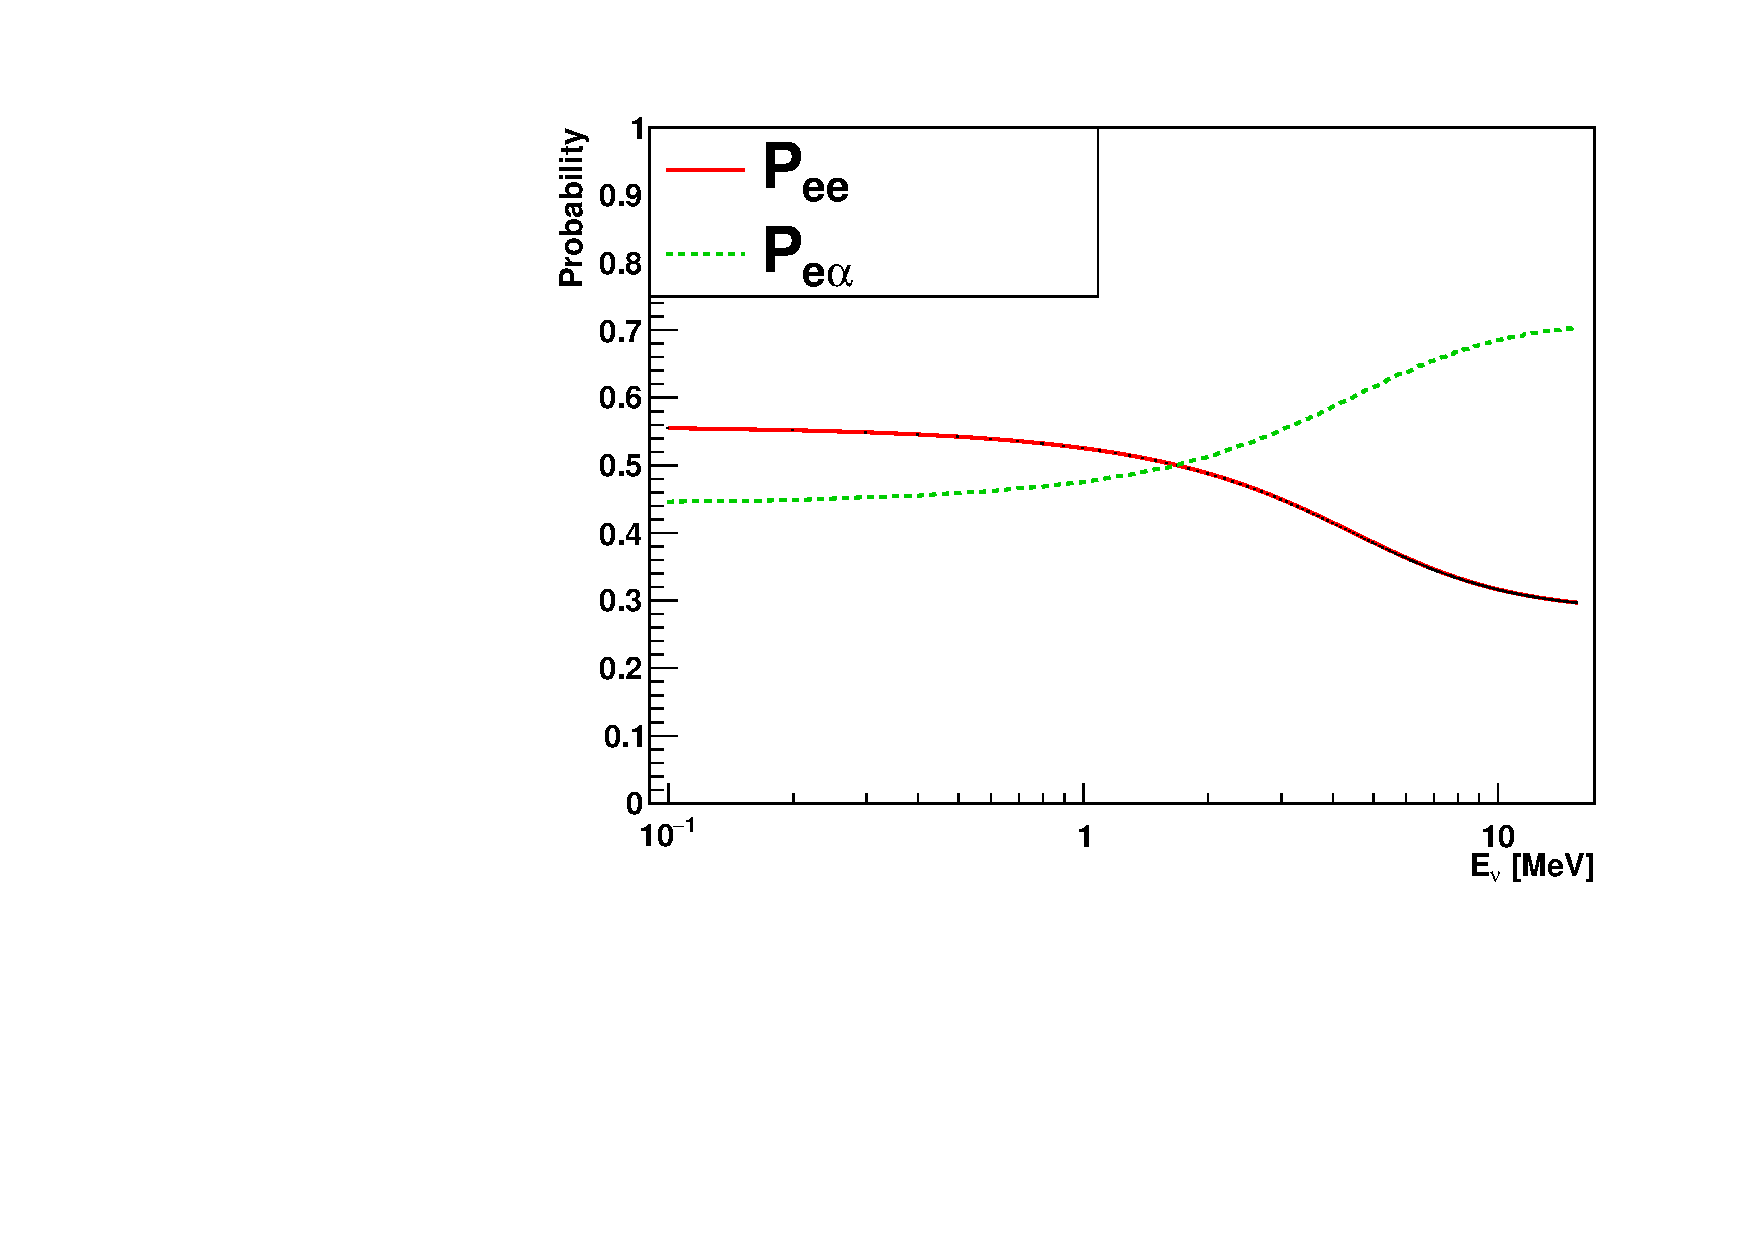
\includegraphics[width=10cm]{PSelmaa_bs05op.pdf}
	\caption[The MSW survival probability curves as functions of MC energies.]{The MSW survival probability curves as functions of MC energy. The $P_{ee}$ is in solid red line and $P_{e\alpha}(=1-P_{ee})$ is in dashed green line.}
	\label{fig:pselmaa_curves}
\end{figure}

In order to enlarge the MC datasets for analysis, the MC simulations of solar neutrinos were produced much larger than the expected numbers. The number of simulated solar $\nu_e$ events is 1700 times the nominal ($\mathrm{flux~scale} = \frac{1}{1700}$); while the number of solar $\nu_\mu$ events is 9600 times the nominal ($\mathrm{flux~scale}=\frac{1}{9600}$). The two $\mathrm{flux~scale}$ factors are prescribed according to the ratio of the ES cross-sections: $\sigma^{ES}(\nu_{e}+e^-)/\sigma^{ES}(\nu_{\mu,\tau}+e^-)\approx 6.5$, as mentioned in Sect.~\ref{sect:NuEStheory}. A nominal $^8$B solar $\nu_e$ flux $\Phi^{total}_{MC}=5.46\times 10^6$~cm$^{-2}$s$^{-1}$ from the SSM prediction (see Refs.~\cite{vinyoles2017new,pdg2020}) is used by the simulation.

Since it is impossible for the SNO+ detector to discriminate between $\nu_\mu$ and $\nu_\tau$ by detecting the elastic scattering events, $\nu_\tau$ is not generated separately \cite{marzec2019measurement}. Therefore, the generated solar $\nu_\mu$ events are considered as a combination of $\nu_\mu$ and $\nu_\tau$ ($\nu_\mu\approx\nu_{\mu,\tau}$) in the solar neutrino flux. In addition, due to the data cleaning procedure, the actual live time of the data is slightly shorter than the raw live time used by the MC simulations. To compare the MC with the data, a live time fraction was applied to the MC: $f_\mathrm{live~time}=\frac{t_\mathrm{data~live~time}}{t_\mathrm{MC~run~time}}=\frac{190.33~days}{198.17~days} = 0.96$. Similarly, assuming a sacrifice of 1.7\% from the data cleaning cuts on the data, a scale factor $f_{dataClean}=(1-\frac{1.7}{100})$ was applied to the MC simulations. Accordingly the numbers of MC-generated $\nu_e$ and $\nu_\mu$ events are scaled by $f_\mathrm{live\, time}$ and $\mathrm{flux~scale}$, then weighted by the oscillation probabilities $P_{ee}$ and $P_{e\alpha}=1-P_{ee}$. Applying these weighting parameters as well as the BDT selections to the MC histograms, the MC $\cos\theta_\mathrm{sun}$ distributions in the energy region $5<E_{fit}<15$ MeV are shown (with and without oscillations) in Fig.~\ref{fig:MCfluxPdfs}.

\begin{figure}[!htb]
	\centering
	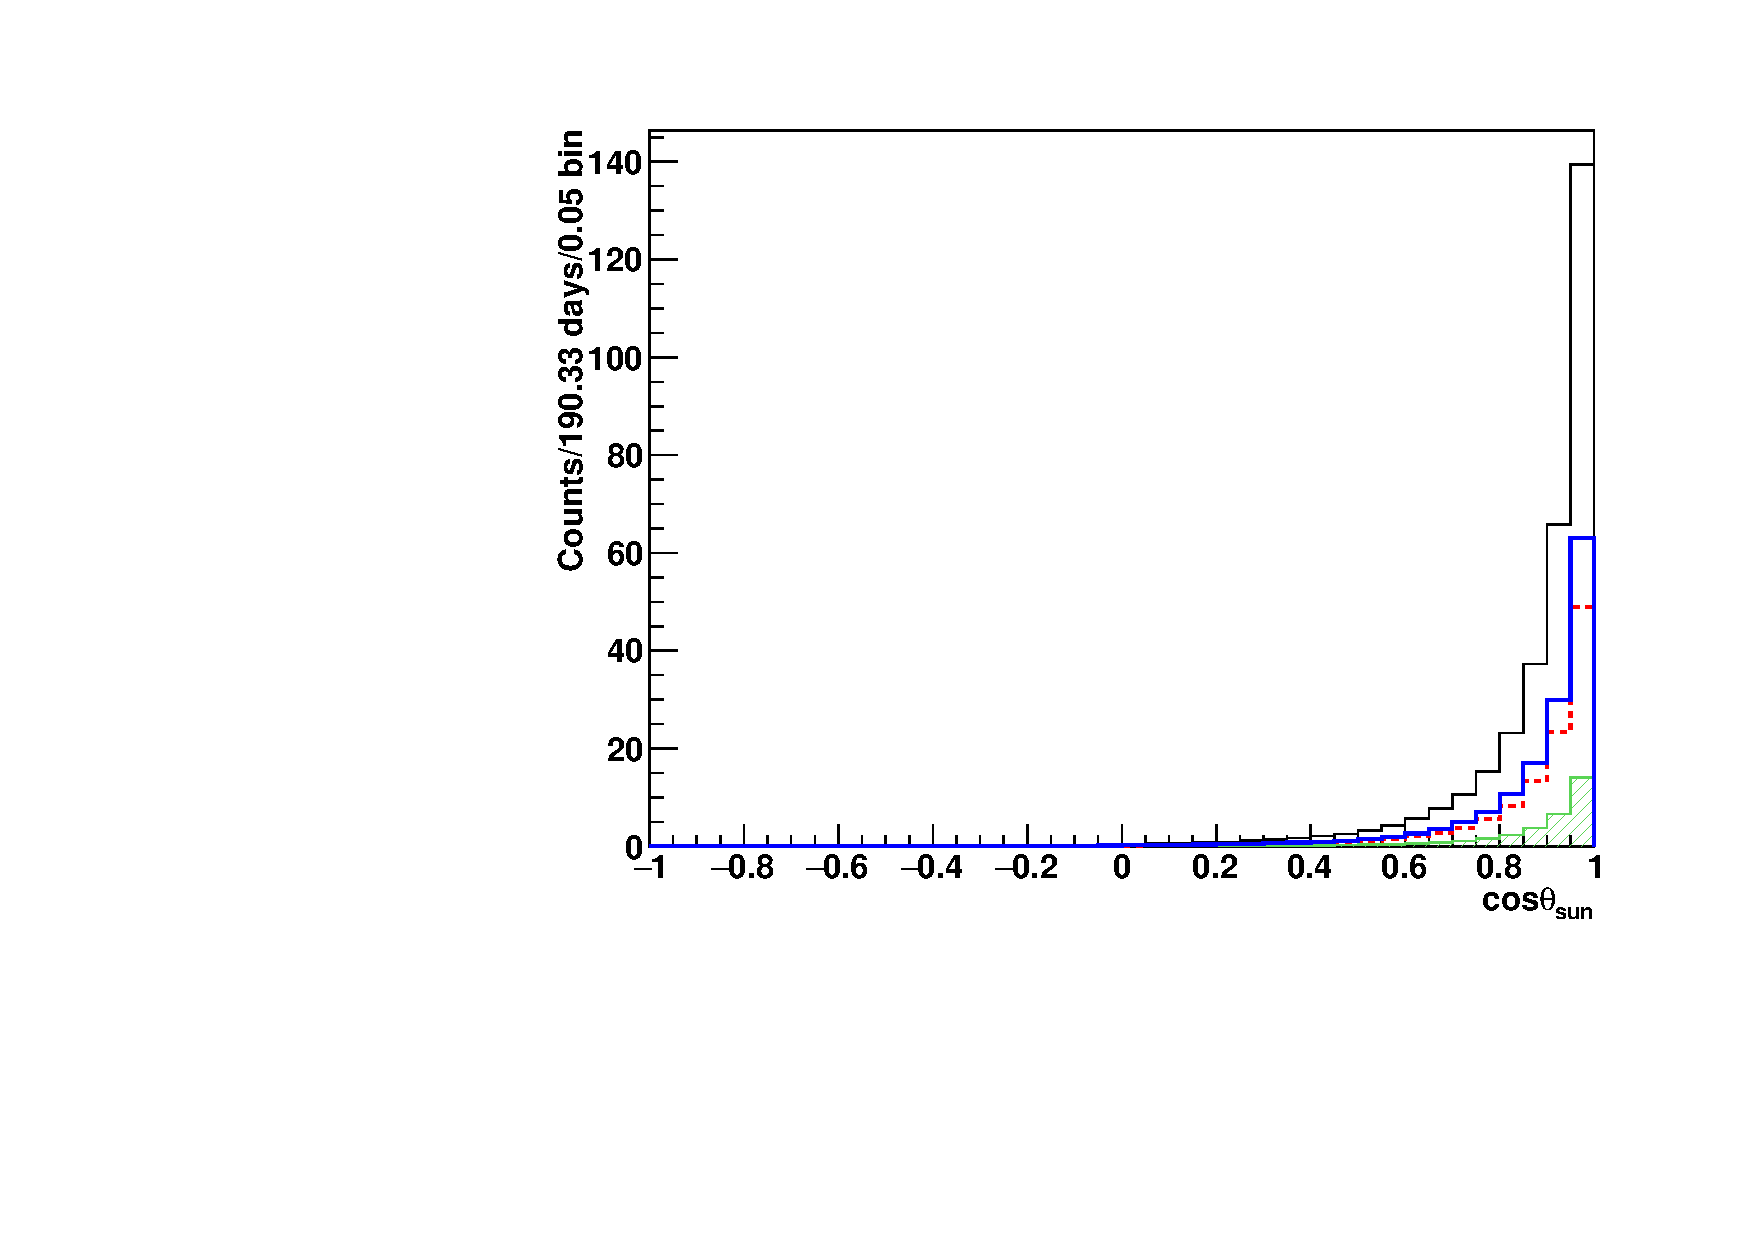
\includegraphics[width=8cm]{MCfluxPdfs.pdf}
	\caption[The MC $\cos\theta_\mathrm{sun}$ distributions used as PDFs for the flux calculations, for $5<E_{fit}<15$ MeV after the BDT selections.]{The MC $\cos\theta_\mathrm{sun}$ distributions used as PDFs for the flux calculations, for $5<E_{fit}<15$ MeV after the BDT selections. The black histogram is the $\nu_e$ flux without oscillation, denoted $PDF(\nu_e, \, \mathrm{without~oscillation})$. This histogram is used for fitting the elastic scattering flux. The histogram in dashed red line is the $\nu_e$ flux and the green shaded histogram is the $\nu_\mu$ flux, both including the oscillation. These two histograms were combined to form the total flux including the oscillation, which is given by the blue line and is denoted by $PDF(\nu_e+\nu_\mu, \, \mathrm{oscillated})$. This (blue) histogram is used for fitting the total flux.}
	\label{fig:MCfluxPdfs}
\end{figure} 

Reading from the above histograms, the expected event count for $\nu_e$ without the oscillation is $N_{\nu_e} = 314.679$. Assuming a flux of $\nu_\mu$, the expected number of $\nu_\mu$ is $N_{\nu_\mu}=49.2741$, then $N_{\nu_e}/N_{\nu_\mu}\approx 6.4$, which is consistent with the ratio of the cross-sections mentioned before. Including the oscillations, the expected event counts for $\nu_e$ and $\nu_\mu$ are $N^{osci}_{\nu_e} = 109.494$ and $N^{osci}_{\nu_\mu} = 32.0757$ respectively, and the combined event count is $N^{osci}_{\nu_e+\nu_\mu}=141.569$. %%%% 
 
To fit for the total $^8$B neutrino flux, the fit parameter used here is the flux scale $f^{tot}_s$, which is interpreted as the fraction of the observed $^8$B flux to the expected flux. Using the same method in Sect.~\ref{sect:poisson_fit}, and in the Eqn.~\ref{eq:solar_poissonFitMinimizer}, replacing the $N_{sig}$ with $N_{sig}=f^{tot}_s\cdot N^{osci}_{\nu_e+\nu_\mu}$(where the estimated $N^{osci}_{\nu_e+\nu_\mu}=141.57$), and then fitting the $f^{tot}_s$ and the $N_{bkg}$ with the $\mathrm{PDF}(\nu_e+\nu_\mu,\mathrm{oscillated})$. The fit results are $f^{tot}_s=0.8462\pm 0.08398$ (corresponding to $N_{sig}=119.8\pm11.89$ events) and $N_{bkg}=38.20\pm7.731$ events, with a p-value of 0.1470. Fig.~\ref{fig:TOTALfluxFit} shows the fit spectrum.

\begin{figure}[!htb]
	\centering
	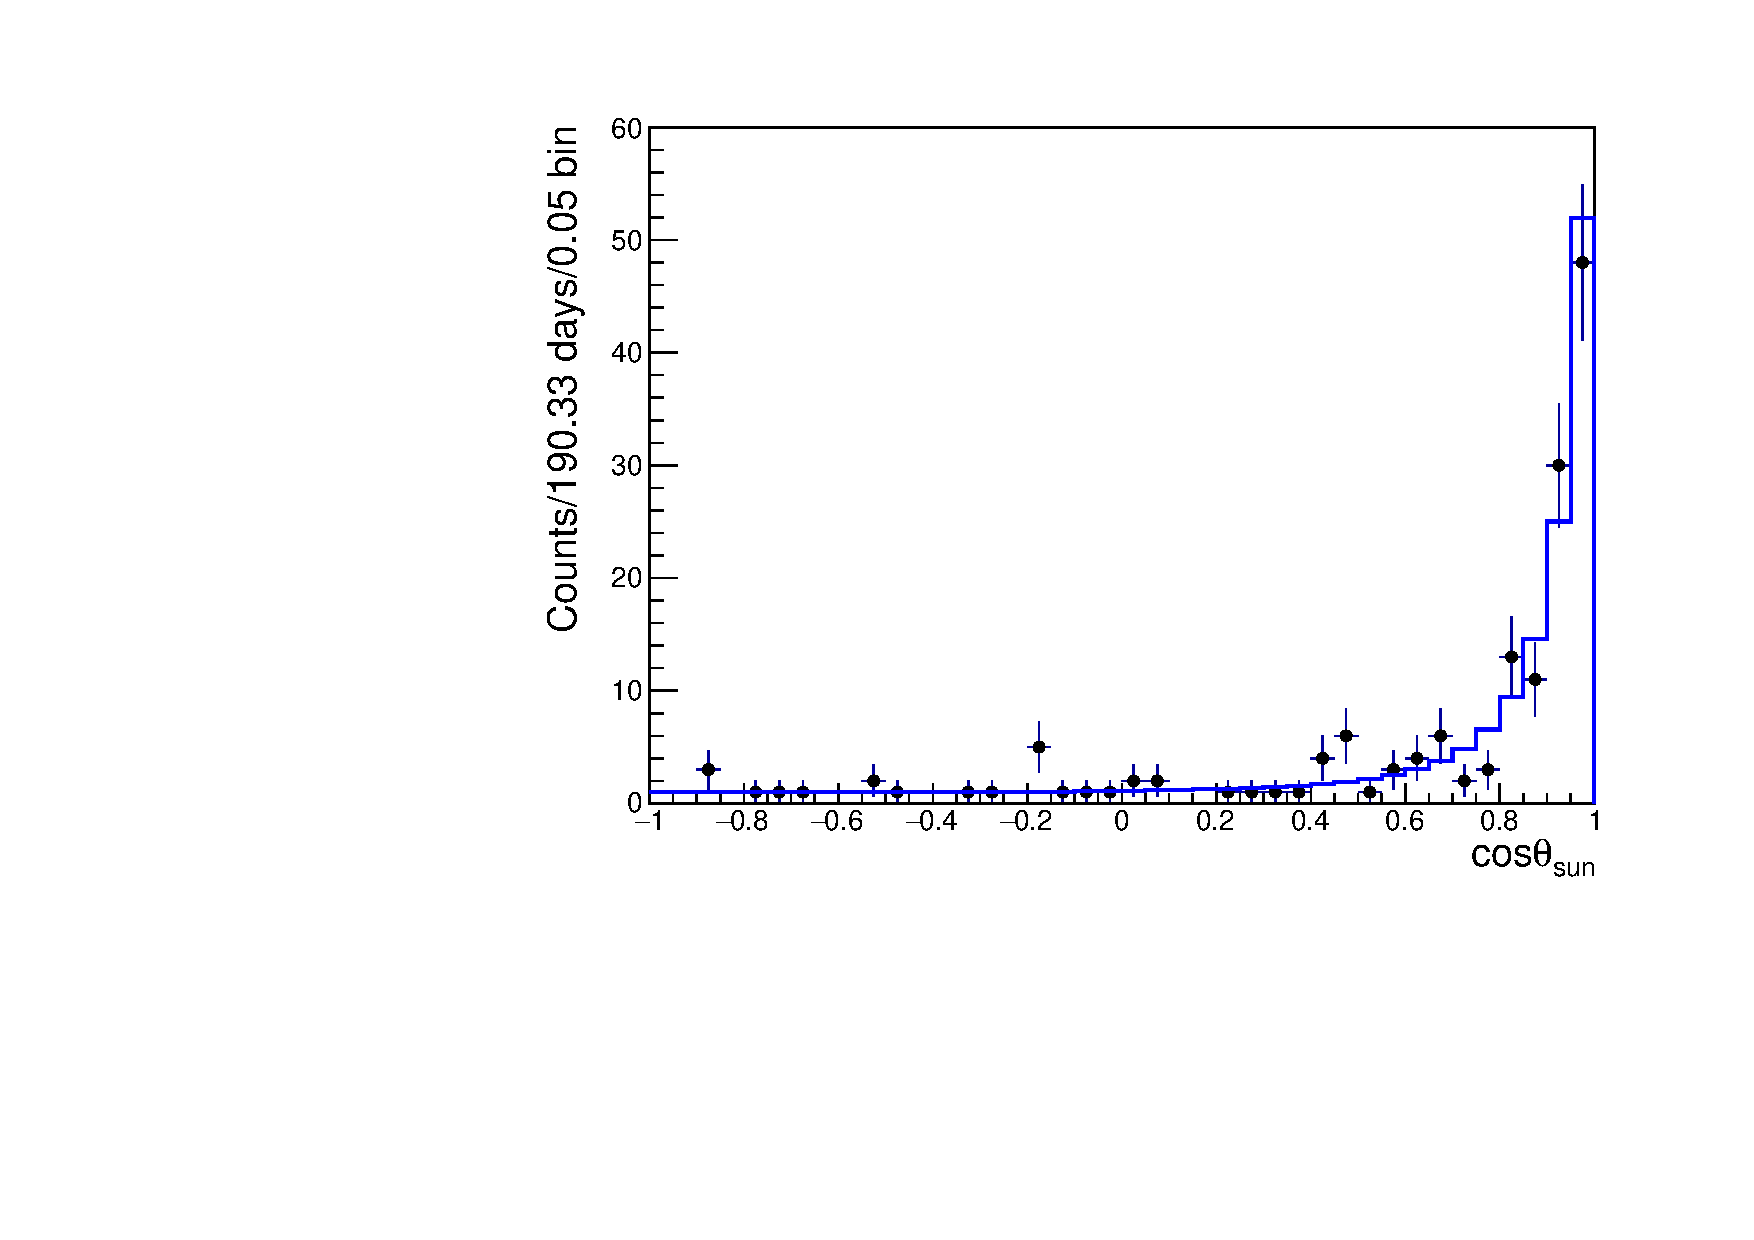
\includegraphics[width=10cm]{TotalFluxFit.pdf}
	\caption[A fit on the total $^8$B flux.]{A fit on the total $^8$B flux. The black dots are the data points and the blue histogram is the fit.}
	\label{fig:TOTALfluxFit}
\end{figure}

To fit for the $^8$B flux corresponding to an observed flux of ES interactions, the same procedure was used, while the fit parameter was changed to $N_{sig}=f_s \; N_{\nu_e}(=314.68)$ and the PDF was changed to $\mathrm{PDF}(\nu_e,\mathrm{without~oscillation})$. As shown in Fig.~\ref{fig:ESfluxFit}, the fit results are $f^{ES}_s=0.3798\pm 0.03772$ (corresponding to $N_{sig}=119.5\pm11.62$ events) and $N_{bkg}=38.48\pm 7.751$ events, with a p-value = 0.140.

\begin{figure}[!htb]
	\centering
	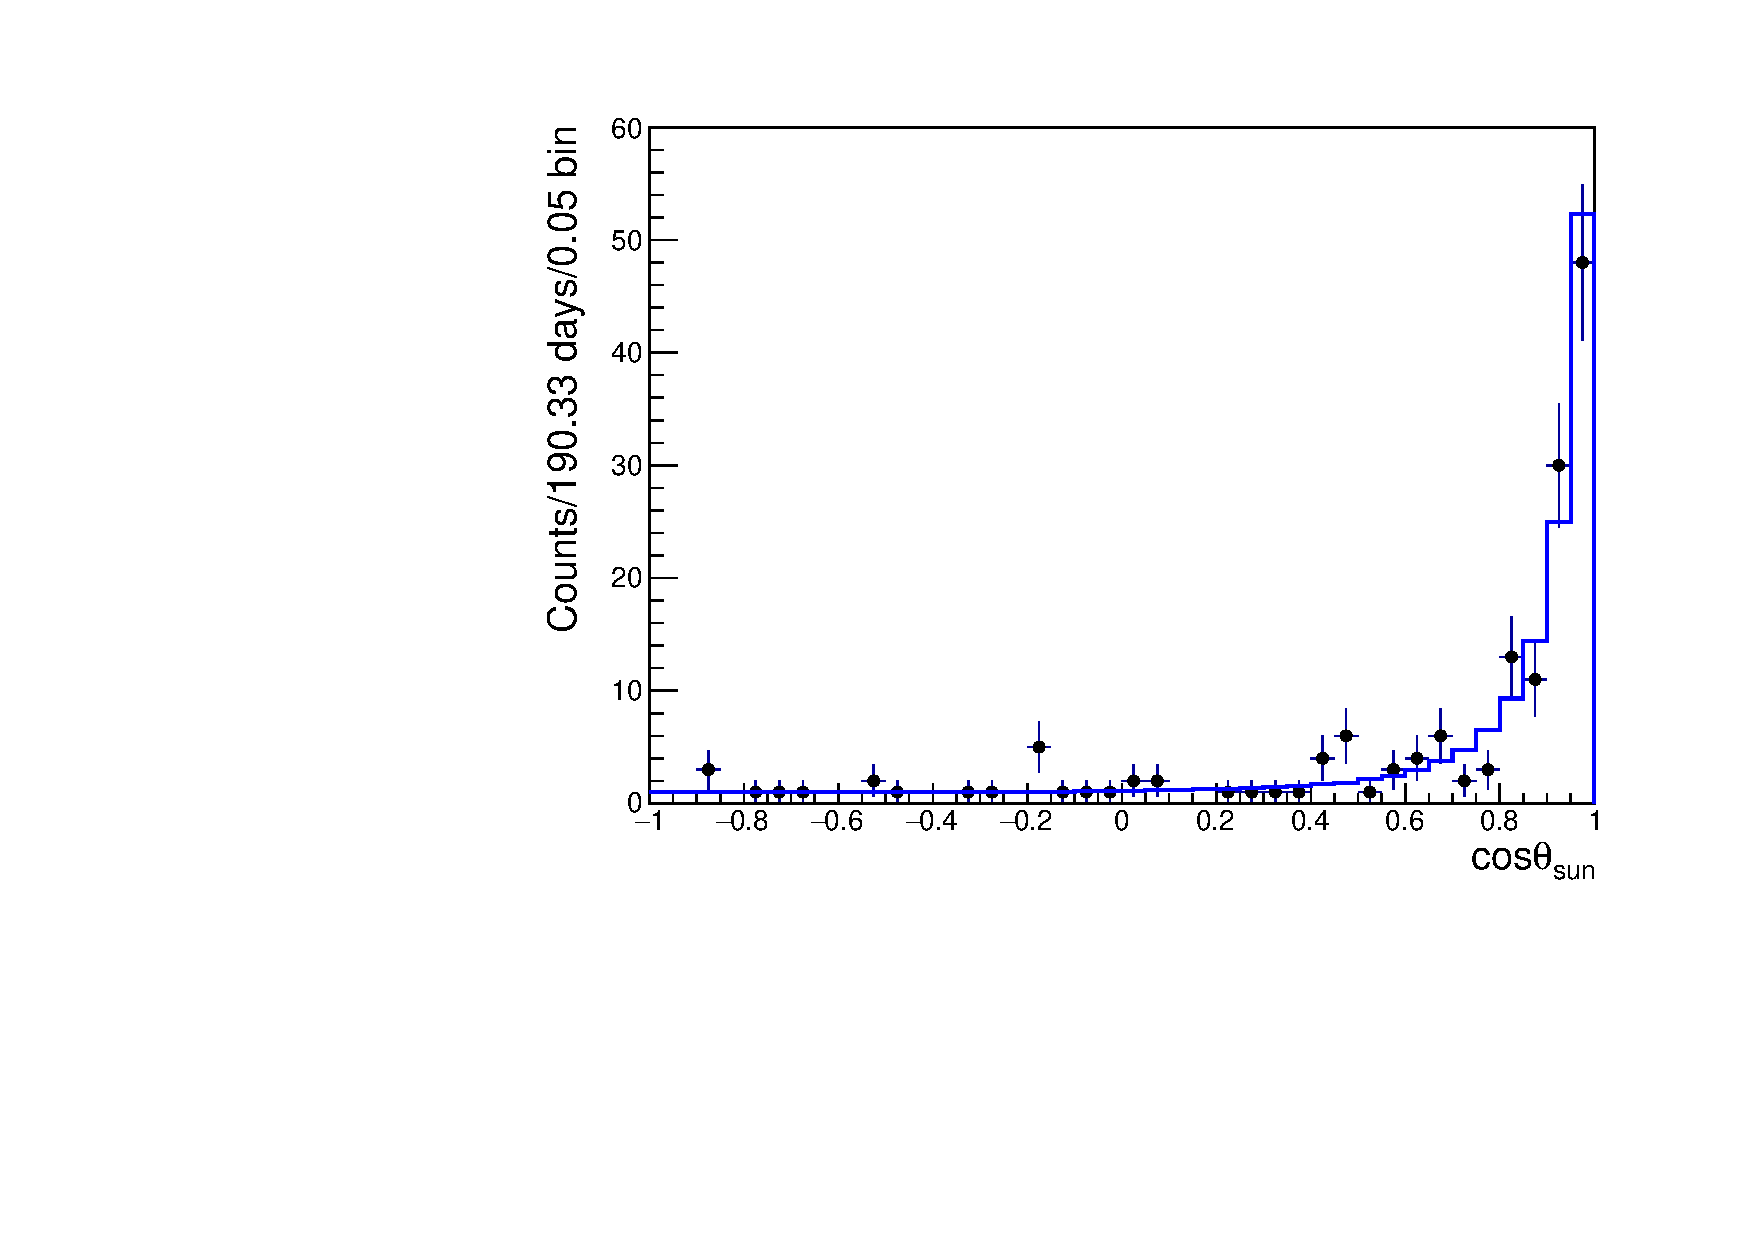
\includegraphics[width=10cm]{ESfluxFit.pdf}
	\caption[Fitting with the spectrum of elastic scattering.]{Fitting with the spectrum of elastic scattering. The black dots are the data points and the blue histogram is the fit.}
	\label{fig:ESfluxFit}
\end{figure}

The $N_{sig}$ and $N_{bkg}$ values obtained here by fitting the flux fractions are consistent with the values obtained in Sect.~\ref{sect:fitTheWhole}.

With the nominal $^8$B solar neutrino flux $\Phi^{total}_{MC}$, the estimated total flux is:

\begin{equation}
\Phi^{total}(\mathrm{^8 B})=f^{tot}_s\cdot \Phi^{total}_{MC}=(4.62 \pm 0.459(stat.))\times 10^6~\mathrm{cm^{-2}s^{-1}},
\end{equation}

and the estimated elastic scattering flux is:
\begin{equation}
\Phi^{ES}=f^{ES}_s\cdot \Phi^{total}_{MC}=(2.074\pm 0.2061(stat.))\times 10^6~\mathrm{cm^{-2}s^{-1}}.
\end{equation}

The next section will evaluate the systematic uncertainties of the flux fractions.

\subsection{Systematics Evaluation}
In Chapter 5, the reconstruction systematics of the event position, direction and energy were obtained. The quantities of position scale, position shifts, direction resolution, $\beta_{14}$ shifts, energy scale ($E_{scale}$) and energy resolution ($E_{resol}$) were used to evaluate the systematic uncertainties of the solar neutrino analysis. Table.~\ref{tab:solar_uncertainties} summarizes these systematics and their applications to transform the reconstructed results. In this thesis, only the systematics mentioned below were taken into account, and these systematics are considered uncorrelated. 

\begin{table}[ht]
	\centering
	\caption{Systematics for the solar $\nu_e$ analysis in the water phase.}
	\label{tab:solar_uncertainties}
	\begin{tabular*}{150mm}{c@{\extracolsep{\fill}}ccc}
		\toprule
		Systematics & values (positive/negative) & transformation   \\
		\hline
		x shift ($\Delta x$) & +6.48/-5.98 mm  & $x_{fit}\pm \Delta x$ \\	
		y shift ($\Delta y$)& +6.13/-4.11 mm   & $y_{fit}\pm \Delta y$ \\
		z shift ($\Delta z$)& +6.71/-4.82 mm   & $z_{fit}\pm \Delta z$ \\
		x scale ($\Delta s_x$)& +0.07\%/-0.06\%  & $(1\pm \Delta s_x)x_{fit}$\\	
		y scale ($\Delta s_y$)& +0.02\%/-0.07\%  & $(1\pm \Delta s_y)y_{fit}$ \\
		z scale ($\Delta s_z$)& +0.08\%/-0.01\%  & $(1\pm \Delta s_z)z_{fit}$ \\
		direction $\delta_\theta$  & +0.013/-0.101 & $1+\frac{\cos\theta_\mathrm{sun}-1}{1\pm\delta_\theta}$\\
		$E_{scale}~(\Delta_{\delta_E})$ &  1.0\%  & $(1\pm \Delta_{\delta_E})E_{fit}$\\
		$E_{resol}~(\Delta_b)$ &  0.037 $\sqrt{\mathrm{MeV}}$  & $E_{fit}+Gaus(0,\sigma_{smear})$, \\
		& &$\sigma_{smear}=\sqrt{E_{fit}}\sqrt{(1+\Delta_b)^2-1}$\\
		$\beta_{14}$ shift ($\Delta \beta_{14}$) & +0.010/-0.036 & $\beta_{14}\pm \Delta \beta_{14}$\\
		\bottomrule
	\end{tabular*}
\end{table}

Note that the position shifts were applied to the $x_{fit},~y_{fit}$, and $z_{fit}$ respectively, while the position scales were applied simultaneously to the position vector: 

$\vec{X'}_{fit}=((1\pm \Delta s_x)x_{fit},(1\pm \Delta s_y)y_{fit},(1\pm \Delta s_z)z_{fit})$.

For $\delta_\theta$, since there is no physical meaning to the case that $\vert \cos\theta_\mathrm{sun} \vert >1$. If the transformation causes $\cos\theta_\mathrm{sun}>1$, the smeared value is reset to 0.999; on the other hand, the $\cos\theta_\mathrm{sun}<-1$ case happens more frequently and is considered to be a consequence of mis-reconstruction. In this case, a random value is chosen by uniformly sampling on the range [-1,1]. This procedure follows Ref.~\cite{waterunidoc}.

To evaluate the systematics of the solar neutrino analysis, the systematic transformations in Table.~\ref{tab:solar_uncertainties} were applied to the reconstructed quantities in MC simulations independently. The reconstructed quantities after the transformations are called ``smeared'' values. The smeared values of an event can affect whether the event will pass the cuts: the smeared positions of an event affect whether the event can pass the fiducial volume cut and then affect the results after the position cuts; the smeared energies affect the results after the energy cuts and the smeared $\beta_{14}$ affect the results after the $\beta_{14}$ cuts. Thus, for the solar $\nu_e$ and $\nu_\mu$ simulations, the shape of the $\cos\theta_\mathrm{sun}$ distribution used as the PDF will be changed by the smeared values. In addition, the $\delta_\theta$ transformation changes the PDF shape directly. Finally, the spectrum of the data was re-fit with the smeared PDFs to obtain the smeared physics quantity (specifically, the flux ratio $f_s$ mentioned in the previous section), and the differences between the original value and the smeared value are used as the systematics of the physics quantity.

To obtain the smeared PDFs, first, only the cuts $5<E_{fit}<15$ MeV (for selecting energy region), NHit$>20$ (reconstruction threshold) and ITR$>0.55$ (determined from the instrumental noises and its systematic uncertainty was not considered) were applied to the MC simulations of the solar $\nu_e$ and $\nu_\mu$. Then the systematic transformations were applied one by one and event by event. For the transformations, the positive (``smearing up'') and negative (``smearing down'') values were applied, respectively. After the transformation, the whole beforehand cut was applied. Lastly, the TMVA BDT selection was applied. For a specific smeared quantity, the final output of the MC $\cos\theta_\mathrm{sun}$ spectrum was used as the smeared PDF for that quantity. For example, if $E_{fit}$ is smeared by scaling up, i.e. $E'_{fit}=(1+\Delta_{\delta_E})E_{fit}$, then the outputs of the $\cos\theta_\mathrm{sun}$ after the beforehand cut and TMVA BDT selection is used as the ``energy scale-up PDF''.

Fig.~\ref{smearESpdfs} shows the effects of smearing the direction parameter, energy scale and energy resolution on the MC PDF. The original MC PDF is shown as black solid line histograms, overlaid by the smeared histograms.

\begin{figure}[htbp]
	\centering
	\subfigure[Smearing direction parameter $\delta_\theta$.]{ 
		\begin{minipage}[t]{0.5\textwidth}
			\centering
			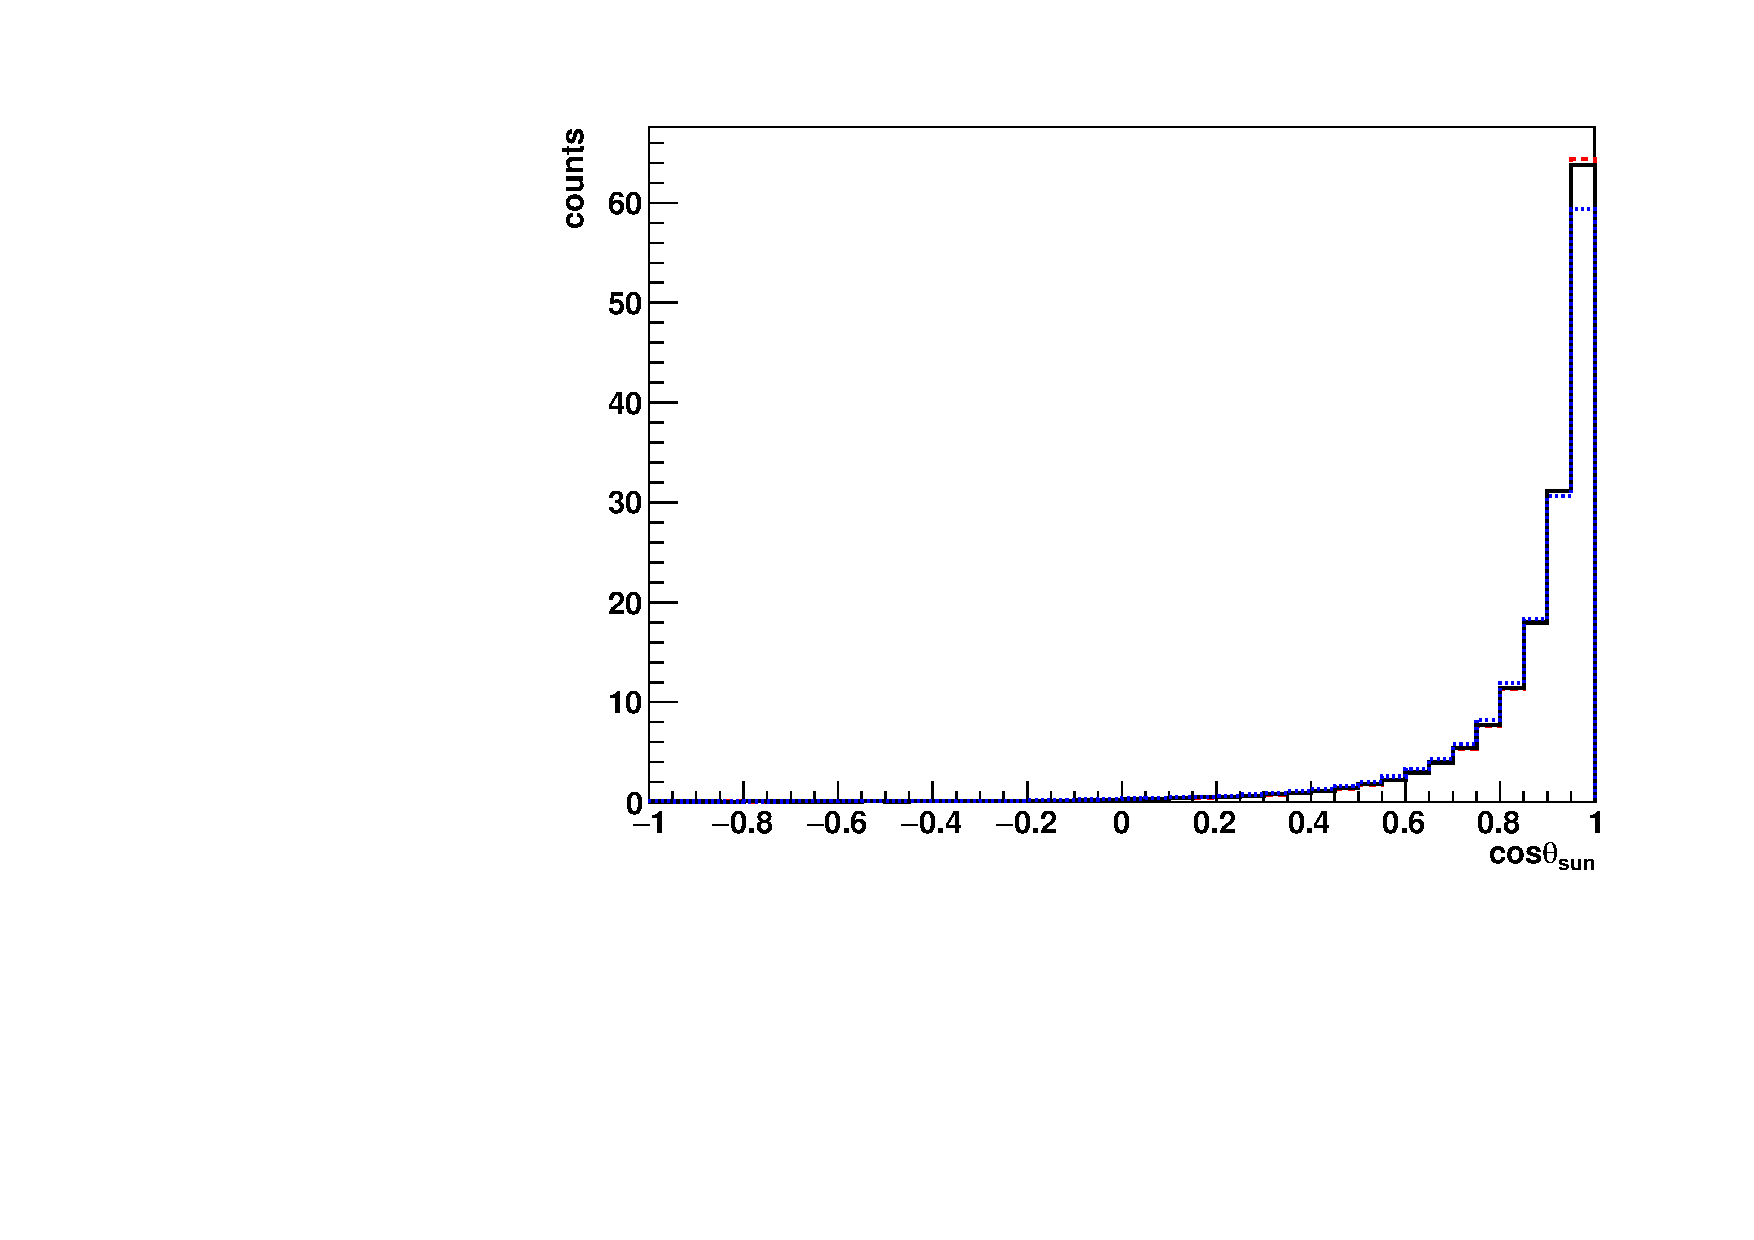
\includegraphics[width=8cm]{smearCosSunPDF_Dir.pdf}
		\end{minipage}
	}
	\subfigure[Smearing energy resolution $\Delta_b$.]{ 
		\begin{minipage}[b]{0.5\textwidth}
			\centering
			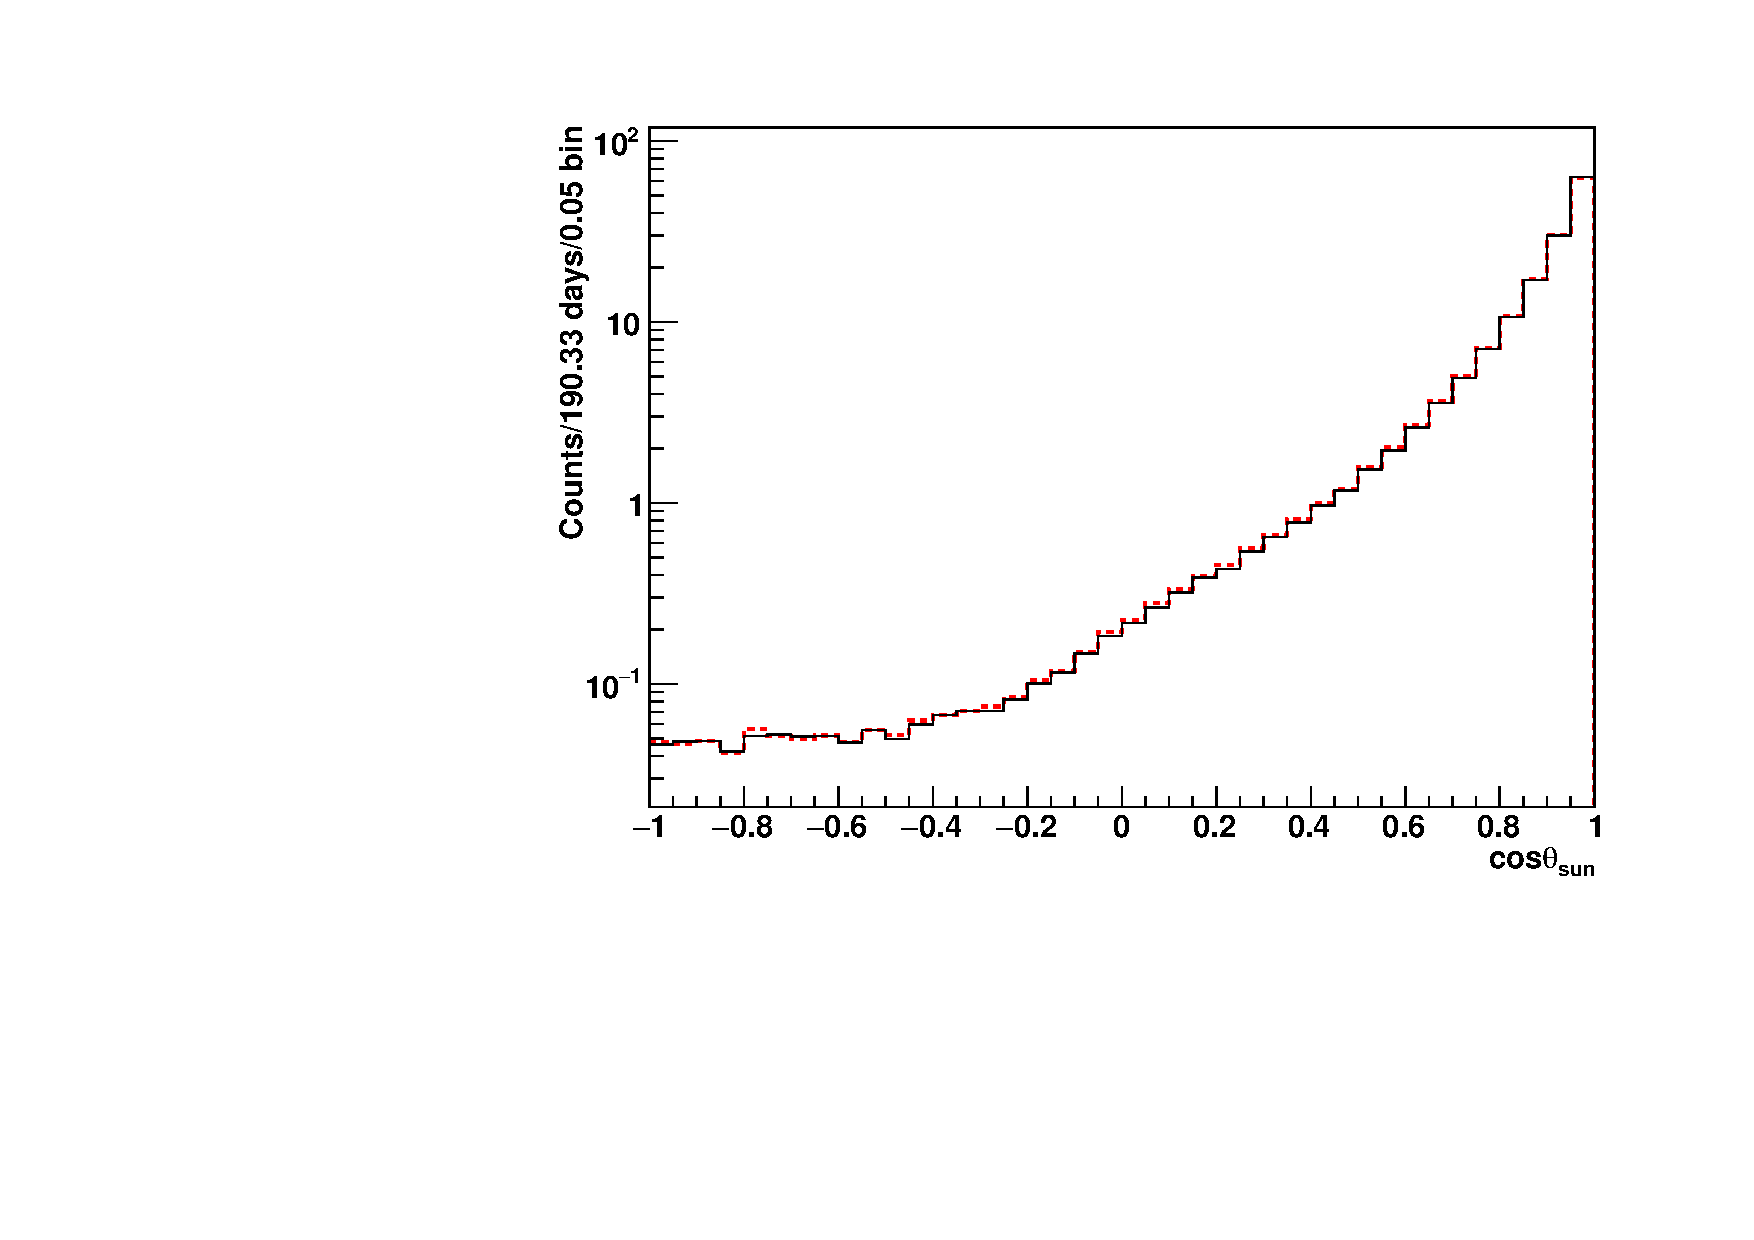
\includegraphics[width=8cm]{smearCosSunPDF_Eresol.pdf}
		\end{minipage}
	}
	\subfigure[Smearing energy scale $\Delta_{\delta_E}$.]{ 
		\begin{minipage}[t]{0.4\textwidth}
			\centering
			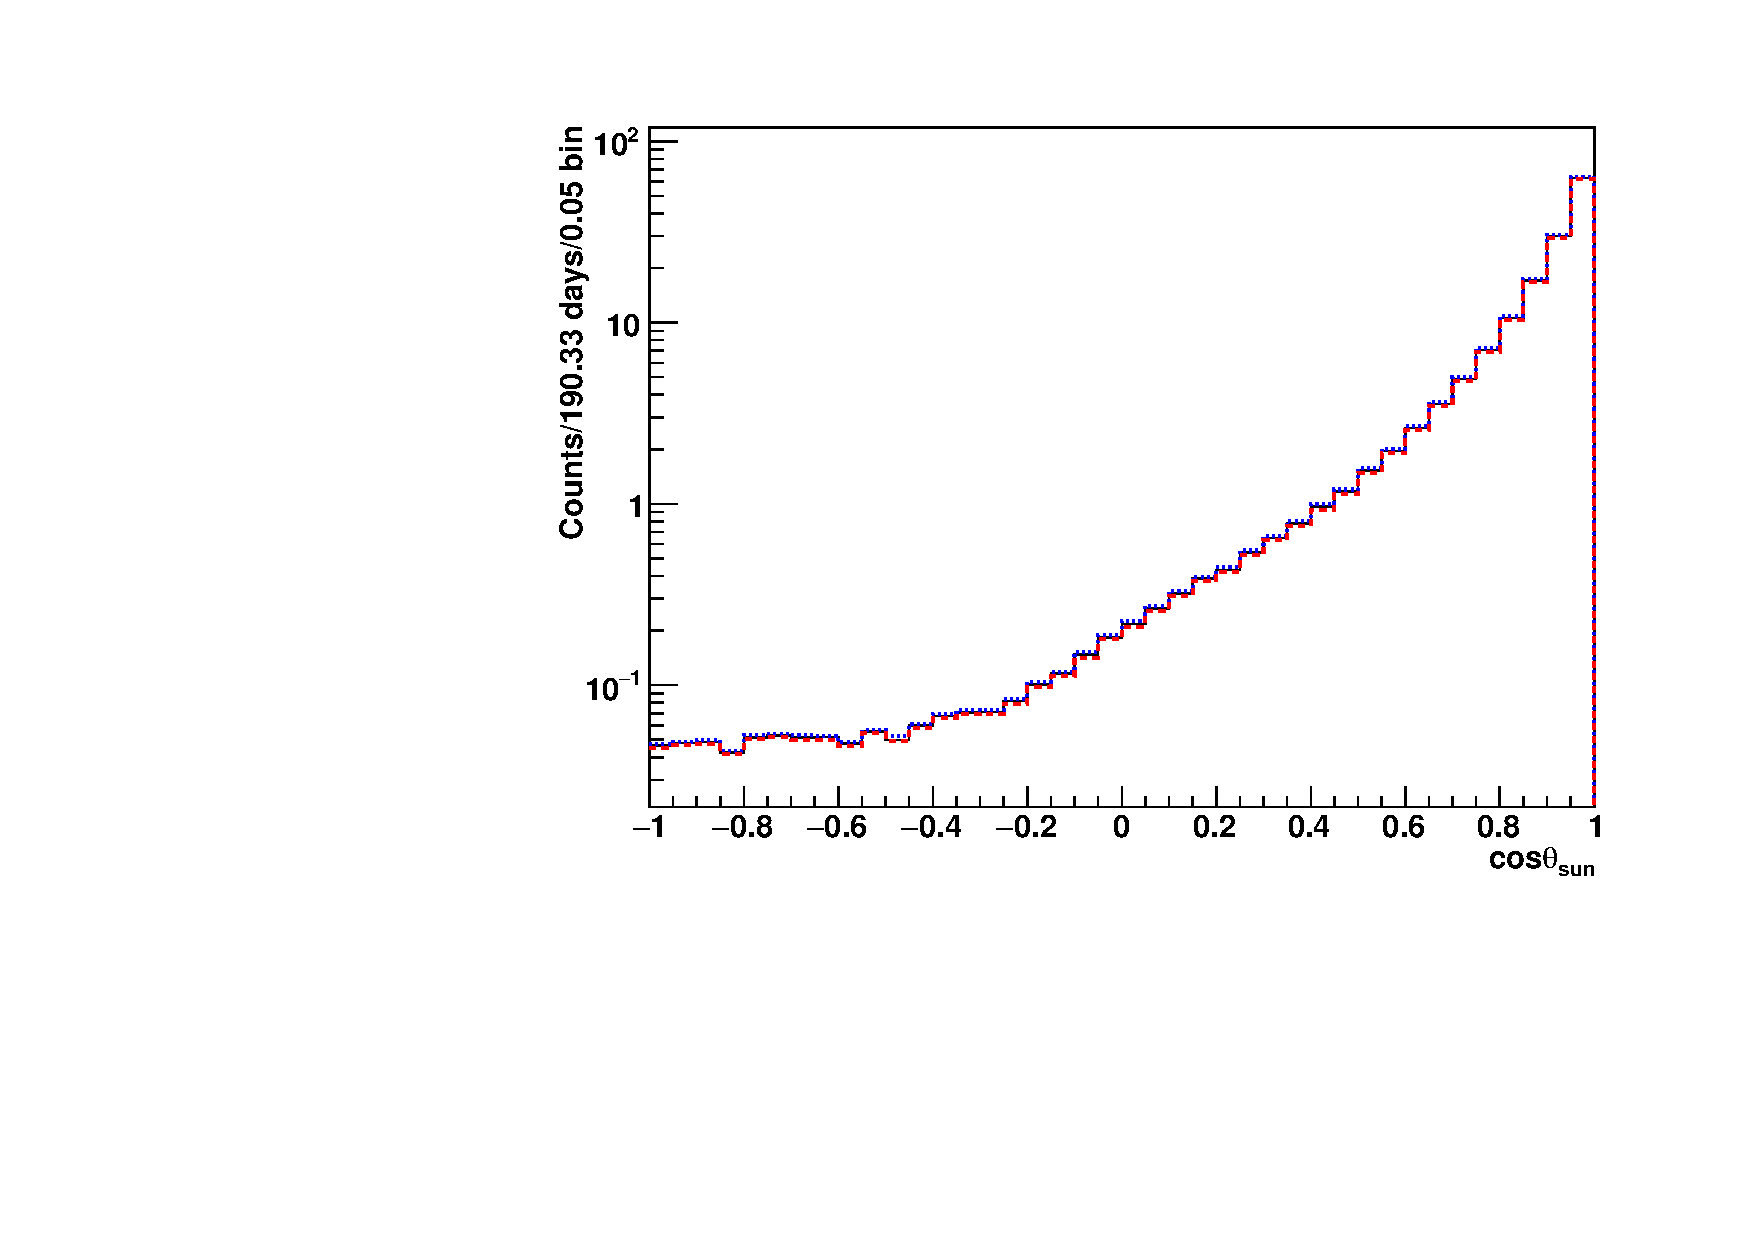
\includegraphics[width=8cm]{smearCosSunPDF_Escale.pdf}
		\end{minipage}
		}
	\caption[Smearing effects on the $\cos\theta_\mathrm{sun}$ PDF.]{Smearing effects on the $\cos\theta_\mathrm{sun}$. The histogram with solid black line is the PDF before smearing. The dotted blue histogram is for smearing up the quantity (i.e., taking the positive values) and the dashed red is for smearing down (i.e., taking the positive values).\label{smearESpdfs}}
\end{figure}   

Applying the systematic transformation in Table.~\ref{tab:solar_uncertainties} to the MC ES PDF, and then refitting the data with the smeared PDFs for each quantity, the smeared values of the flux fractions ($f'_s$) were found. The systematics of the $f_s$ are calculated by $\Delta f_s =f'_s-f_s$. These results are listed in Table.~\ref{tab:smearingResults}. Summarising, the systematic uncertainties from the smeared position and $\beta_{14}$ are negligible, while those resulting from smearing the direction and energy result in more significant uncertainties. 
\begin{table}[ht]
	\centering
	\caption{Systematics for the fitted flux scale $f_s$.}
	\label{tab:smearingResults}
	\begin{tabular*}{80mm}{c@{\extracolsep{\fill}}cc}
		\toprule
		Systematics & $\Delta f_s$ (+/-)\\
		\hline
		x shift & $+0.001891/-0.001962$\\	
		y shift & $+0.001888/-0.001955$\\
		z shift & $+0.002071/-0.001818$\\
		position scale & $+0.000583/-0.00306$\\\	
		$\delta_\theta$  &$+0.01676/-0.004034$\\		
		$E_{scale}~(\Delta_{\delta_E})$ & $+0.01456/-0.01752$\\
		$E_{resol}~(\Delta_b)$ & $+0.003363/-0.003363$ \\
		$\beta_{14}$ shifts & $+0.003968/-0.003285$\\
		\bottomrule
	\end{tabular*}
\end{table}

Using the quadrature sum ($\sigma^2_{tot}=\sum_i \sigma^2_i$) which assumes that all the systematic variables are independent, the total systematic uncertainty of the total flux fraction $f^{tot}_s$ is expected to be: $({f^{tot}_s})^{+0.02306}_{-0.01912}$. Using the same procedure to evaluate the systematics of the elastic scattering flux fraction $f^{ES}_s$ gives $({f^{ES}_s})^{+0.009655}_{-0.008305}$.

\subsection{A Summary of Results} \label{sect:solarESresults}

With the systematic uncertainties of the flux fractions obtained from the previous section, the total flux is:
\begin{equation}
{\Phi^{total}_{fit}(\mathrm{^8 B})=f_s\cdot \Phi^{total}_{MC}=(4.62\pm 0.459(stat.)^{+0.126}_{-0.104}(syst.))\times 10^6~\mathrm{cm^{-2}s^{-1}}},
\end{equation}
while the ES flux is:
\begin{equation}
\Phi_{\mathrm{ES}}=f_s\cdot \Phi^{total}_{MC}=(2.07\pm 0.206(stat.)^{+0.0527}_{-0.0454} (syst.))\times 10^6~\mathrm{cm^{-2}s^{-1}}.
\end{equation}

A quadratic total uncertainty $\sigma_{tot}$ is calculated by combining the larger uncertainties in statistics and systematics:
\begin{equation}
\sigma_{tot}=\sqrt{\sigma^2_{stat,larger}+\sigma^2_{sys,larger}}.
\end{equation}

Fig.~\ref{fig:ESfluxCompare} shows a comparison of the $\Phi_{ES}$ results given here to recent measurements from other experiments (mentioned in Sect.~\ref{sect:solarNu}, Chapter 2), including the SNO+ water phase measurement published in 2018 \cite{anderson2019measurement}, the Super-K phase-IV measurement (Super-K IV) and the combined four phases measurement (Super-K combined) \cite{abe2016solar}, and the Borexino measurements published in 2020 (Borexino 2020) \cite{agostini2020improved}.

\begin{figure}[!htb]
	\centering
	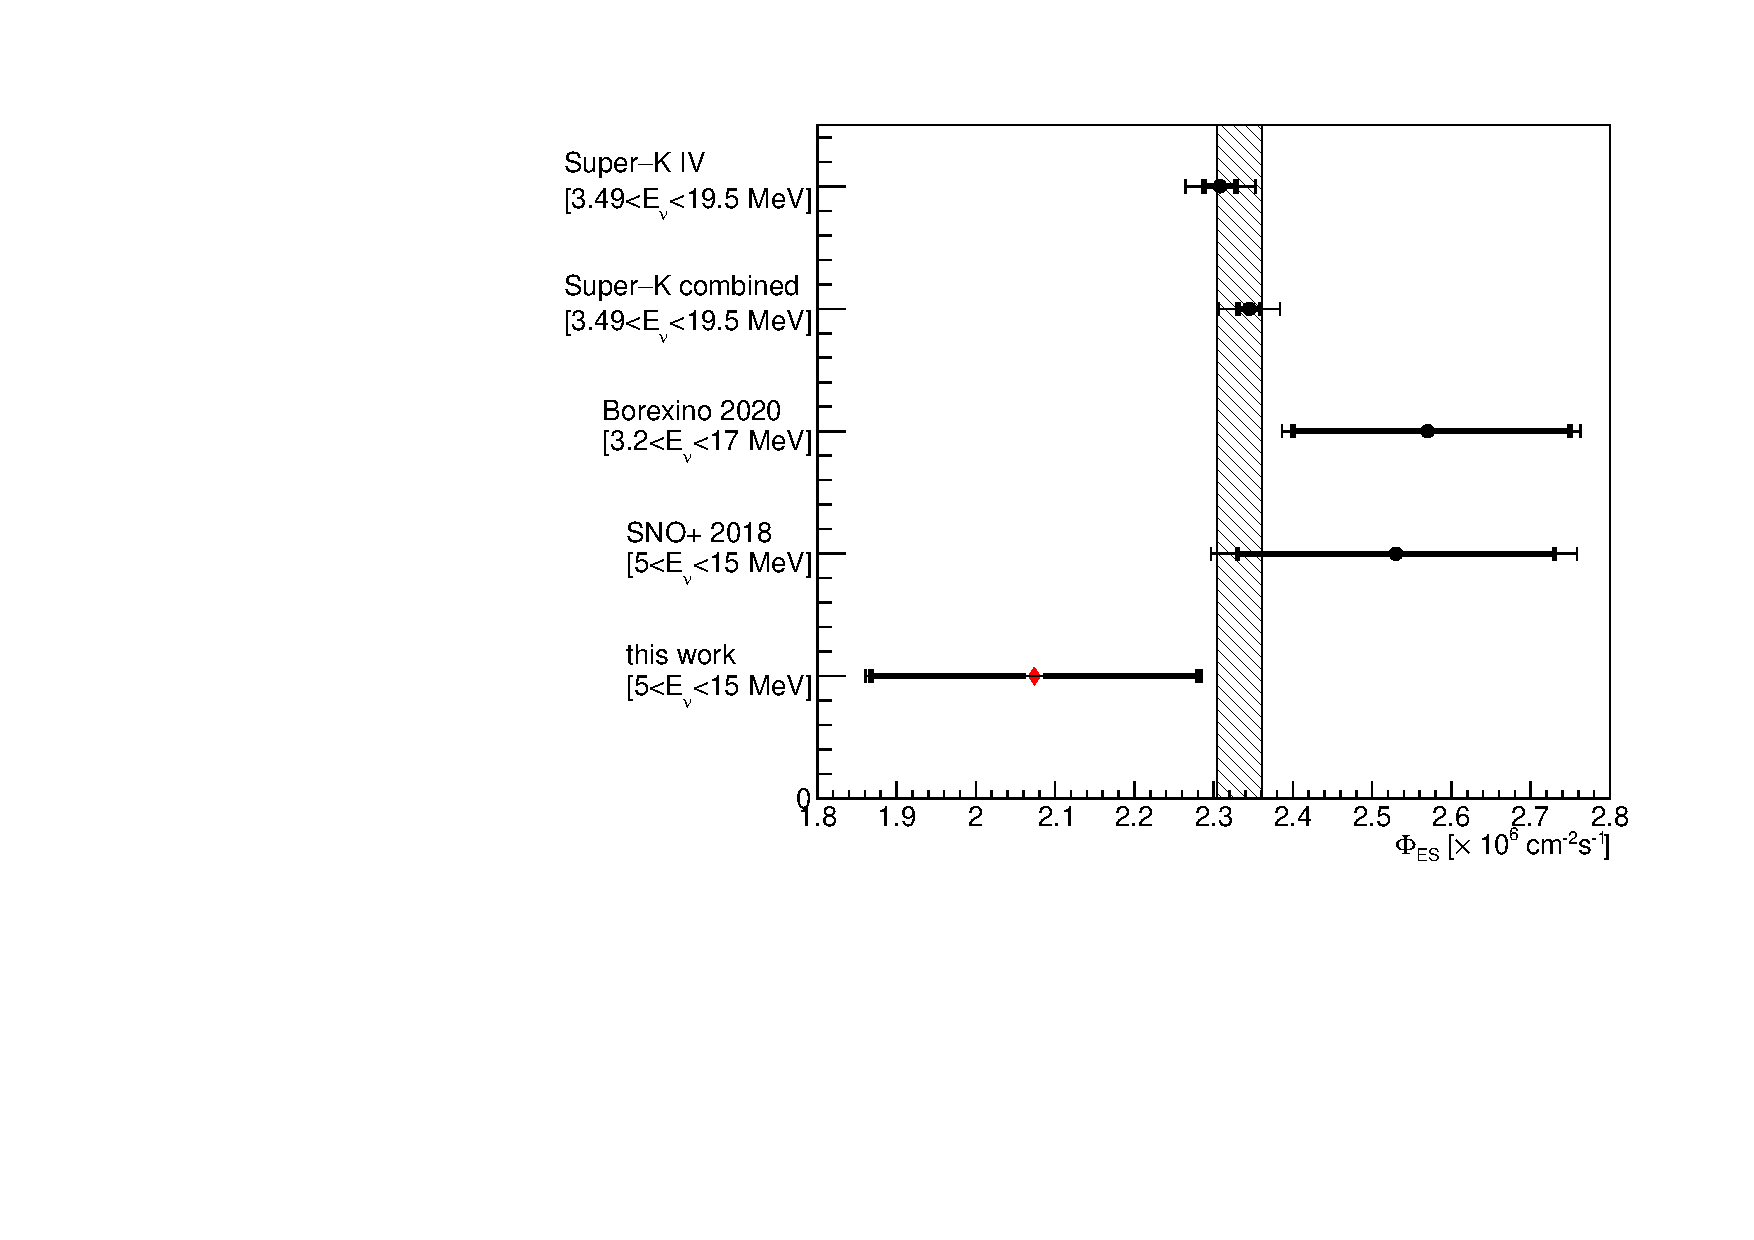
\includegraphics[width=12cm]{ESfluxCompare.pdf}
	\caption[A comparison of the ES flux measured recently by three independent experiments (after BDT selection).]{A comparison of the ES fluxes measured recently by three independent experiments (after BDT selection). The thick error bars include the statistical errors and the thin ones are quadratic errors including both the statistical and systematical errors. The shaded band is for the unconstrained average value and uncertainty of all the results: $\hat \theta \pm 1\sigma_{\hat \theta}$.}
	\label{fig:ESfluxCompare}
\end{figure}

To combine the results from different experiments, an unconstrained average value $\hat \theta$ and its uncertainty $\sigma_{\hat\theta}$ are calculated by \cite{pdg2020,behnke2013data}:
\begin{equation}
\hat \theta = \sum_{i=1}^{N} \left(\frac{x_i}{\sigma_i^2}\right)\Biggm/\sum_{i=1}^{N}\left(\frac{1}{\sigma_i^2}\right),
\end{equation}

\begin{equation}
\sigma_{\hat\theta} =\left[\sum_{i=1}^{N}\left(\frac{1}{\sigma_i^2}\right) \right]^{-\frac{1}{2}},
\end{equation}
where $x_i$ is the measured $\Phi_{ES}$ value from each experiment, and the $\sigma_i$ is the total uncertainty $\sigma_{tot}$ calculated from each experiment. 

Combined with the results from other experiments, the average results are listed in Table.~\ref{tab:ESaverage}.
The $\Phi_{ES}$ result from this thesis is combined with the SNO+ 2018 result and then with all the other experiments' results. The average result without this work is shown in the same plot. All the three average results are consistent with each other.

\begin{table}[ht]
	\centering
	\caption{Average results.\label{tab:ESaverage}}
	\begin{tabular*}{100mm}{c@{\extracolsep{\fill}}cc}
		\toprule
		Combinations & $\Phi_{ES}$ ($\times 10^6$ cm$^{-2}$s$^{-1}$)\\
		\hline
		 not including this work & $2.338 \pm 0.02868$\\
         this work and SNO+ 2018 & $2.281 \pm 0.1571$\\
         all & $2.333\pm0.02843$\\
		\bottomrule
	\end{tabular*}
\end{table}

From the average result including all the experiments mentioned, the region of $\hat \theta\pm 1\sigma_{\hat\theta,tot}$ is plotted as the shaded band in Fig.~\ref{fig:ESfluxCompare}.

\subsection{Limitations of this Study}
This study focuses on measuring solar neutrinos in the energy region [5,15] MeV with a fiducial volume of 5.5 m.

As listed in Table.~\ref{table:mixed_MC}, I only used the $^{208}$Tl and $^{214}$Bi backgrounds simulated in three detector components. The other sources of backgrounds were not included, such as the radio-isotopes in AV ropes and PMTs (etc.) and cosmic muon induced isotopes. A more comprehensive study would be required if one wished to simulate and account for all possible background events.

To fit the background events, I assumed a flat distribution of $\cos\theta_\mathrm{sun}$. A more realistic distribution could be investigated to more properly describe the backgrounds. Furthermore background levels might vary over time, so a more detailed analysis including different time intervals would increase confidence that the present results are representative.

The evaluation here of systematic uncertainties is not comprehensive. In particular, uncertainties intrinsic to the solar neutrino model used by the MC simulations to `produce' solar neutrinos and apply oscillations are {\em not included} here. The uncertainties in the SSM model as well as the neutrino flavor transformation parameters can affect the MC simulations. In addition, the energy calibration used to mitigate the difference between data and simulations is not applied. This procedure can reduce the uncertainties from the energy reconstructions. 

Since the dataset used here has a very low level of background events, it is possible to probe the energy region down to 3.5 MeV, enabling the study of the solar neutrinos in a lower energy region. However since the reconstruction threshold was set as NHits$>20$, that analysis is not included in the thesis. It may be worthwhile to investigate the data with a lower NHit threshold down to NHits$>6$, and to apply a proper TMVA method selection for reducing the backgrounds in the lower energy region.
